%!TEX encoding = UTF-8 Unicode
%!TEX program = xelatex

\documentclass[doctor]{ustcthesis}
% bachelor|master|doctor [professional] [english] [pdf] [authoryear|numebers]
\usepackage{ustcextra}
\graphicspath{{figures/}}

\title{基于软硬件结合方法处理稀疏神经网络的不规则性}
\author{周徐达}
\major{计算机系统结构}
\supervisor{周学海\ 教授}
\cosupervisor{王超\ 副教授}
% \date{二〇一七年五月一日}    % 注释掉则为今日
% \professionaltype{专业学位类型}
% \secrettext{机密\quad 小于等于20年}    % 内部|秘密|机密,注释本行则不保密

\entitle{Addressing Irregularity in Sparse Neural Networks: A Cooperative Software/Hardware Approach}
\enauthor{Xuda Zhou}
\enmajor{Computer Architecture}
\ensupervisor{Prof. Xuehai Zhou}
\encosupervisor{Prof. Chao Wang}
% \endate{May 1, 2017}    % today if commented
% \enprofessionaltype{Professional degree type}
% \ensecrettext{Confidential\quad Less than or equal to 20 years}
% Internal|Secret|Confidential

\begin{document}

\maketitle

% 本科论文:
%   frontmatter: 致谢、目录、中文摘要、英文摘要
%   mainmatter: 正文章节、参考文献
%   appendix: 附录
%
% 硕博论文:
%   frontmatter: 中文摘要、英文摘要、目录、符号说明
%   mainmatter: 正文、参考文献
%   appendix: 附录
%   backmatter: 致谢、发表论文

\frontmatter
%!TEX root =  ../main.tex

\begin{abstract}

神经网络已经在图像识别、目标检测、语音识别和自然语言处理等诸多领域受到广泛应用,并逐渐成为主导算法。然而,随着神经网络的拓扑结构朝着规模不断扩大,层数不断加深的方向发展,庞大的数据和计算量给传统计算平台带来巨大的挑战。虽然稀疏(包括神经元和权值稀疏)能够有效减少神经网络的参数,从而减少数据访问和计算量,但是同时会将稠密网络规则的拓扑结构转化为稀疏不规则的形式,从而阻碍处理平台,包括CPU、GPU和加速器充分利用稀疏特性获得性能的提升。

在本文中,我们提出了一个软硬件结合的方法来有效处理稀疏神经网络不规则的问题。

首先,基于大量的实验,我们观察到了局部收敛的现象,即在训练过程中,权值的分布并不是随机的,大的权重往往会聚集成簇。基于这个关键的观察,我们提出粗粒度的剪枝,大幅降低稀疏神经网络的不规则性。我们提出的粗粒度剪枝将多个突触作为一个整体进行裁剪,而不是裁剪单个突触。我们首先将突触分为多个块,当某个块满足特定条件时,该块中的所有突触将从网络拓扑中永久剪除。然后,我们对经过粗粒度剪枝的神经网络进行重训练保证网络的精度。值得注意的是,我们对神经网络迭代使用粗粒度剪枝和重训练,从而获得理想的稀疏度和精度。粗粒度剪枝可以将稀疏神经网络的不规则度平均减少20.13倍。同时我们提出了一种新的神经网络压缩算法,算法包括粗粒度剪枝,局部量化和熵编码三个步骤,在AlexNet和VGG16上分别获得了79倍和98倍的压缩比,远高于现有的两个最先进的神经网络压缩方法,即Deep Compression(35倍和49倍)和CNNPack(39倍和46倍)。

我们进一步设计了一个新型硬件加速器Cambricon-S,用于有效处理剩余的稀疏神经元和突触的不规则性。新型加速器中最重要的特征是一个中枢神经元选择模块(NSM),它能够有效处理粗粒度突触稀疏。同时,加速器中的突触选择器模块(SSM),Encoder和权值解码模块(WDM)能够分别利用神经元稀疏,动态压缩神经元和利用局部量化。与最先进的稀疏的神经网络加速器Cambricon-X相比,我们的加速器能够获得1.71倍的性能提升,同时减少1.75倍能耗。为了减轻程序员的编程负担,我们还提出一个基于库的编程框架。编程框架中的编译器能够应用loop tiling和数据重用策略生成高效的加速器指令。

  \keywords{神经网络,稀疏,压缩,加速器}
\end{abstract}

\begin{enabstract}
Neural networks have become the dominant algorithms rapidly as they achieve state-of-the-art performance in a broad range of applications such as image recognition, object detection, speech recognition and natural language processing. However, neural networks keep moving towards deeper and larger architectures, posing a great challenge to the huge amount of data and computations. Although sparsity has emerged as an effective solution for reducing the intensity of computation and memory accesses directly, irregularity caused by sparsity (including sparse synapses and neurons) prevents processing platforms, including CPU, GPU and accelerators from completely leveraging the benefits. 

In this paper, we propose a cooperative software/hardware approach to address the irregularity of sparse neural networks efficiently. 

Initially, based on a wide range of experiments, we observe the local convergence, namely larger weights tend to gather into small clusters during training rather than randomly distributed. Based on that key observation, we propose a software-based coarse-grained pruning technique to reduce the irregularity of sparse synapses drastically. Instead of pruning synapses independently, our proposed coarse-grained pruning prunes several synapses together. The synapses are firstly divided into blocks; a block of synapses will be permanently removed from the network topology if it meets specific criteria. We then employ the fine-tuning approach to retain the network accuracy. Note that we apply the coarse-grained pruning iteratively in training to achieve better sparsity and avoid the accuracy loss. The coarse-grained pruning can reduce the irregularity by $20.13\times$ on average. Then we introduce a novel compression algorithm, a three stage pipeline: coarse-grained pruning, local quantization and entropy encoding, that work together to reduce the storage requirement of AlexNet and VGG16 by $79\times$ and $98\times$, respectively. The compression ratio is much higher than that achieved by two existing state-of-the-art neural network compression methods, i.e., Deep Compression ($35\times$ and $49\times$) and CNNPack ($39\times$ and $46\times$).

We further design a hardware accelerator named Cambricon-S to address the remaining irregularity of sparse synapses and neurons efficiently. The novel accelerator features a central neural selector module (NSM) to leverage coarse-grained sparsity. Additional the synapse selector module (SSM), Encoder and weight decoding moduel (WDM) are used to leverage neuron sparsity, dynamically compress the neurons and leverage local quantization, respectively. Compared with a state-of-the-art sparse neural network accelerator Cambricon-X, our accelerator is $1.71\times$ and $1.75\times$ better in terms of performance and energy efficiency, respectively. To ease the burden of programmers, we also propose a high efficient library-based programming environment for our accelerator. The compiler is able to apply loop tiling and data reuse strategies for highly efficient instructions. 

  \enkeywords{neural networks, sparsity, compression, accelerator}
\end{enabstract}

\tableofcontents
% \listoffigures
% \listoftables
% \listofalgorithms
% \input{chapters/0.notation}

\mainmatter
\chapter{绪论}
\citestyle{numbers}

作为现代人工智能的最重要的分支,人工神经网络(artificial neural network, ANN)近年来获得迅速发展。学术界不断提出新的神经网络理论,算法和结构,提高网络模型的表征能力和性能,从而解决各类人工智能问题;
工业界也相继将神经网络应用于目标检测,语音识别,自动驾驶等领域。然而随着神经网络解决的问题越来越复杂,神经网络也朝着规模越来越大,拓扑结构越来越复杂,层数越来越深的方向发展,因此神经网络需要庞大的存储资源,计算资源和能耗完成运算,这不仅给传统的处理平台如CPU和GPU带来巨大的挑战, 而且导致神经网络应用无法部署到嵌入式设备或者移动智能设备中。

研究者从软件和硬件两个方面来来试图解决这个问题。一个方面, 近些年来,研究者利用稀疏(sparsity),量化(quantization),矩阵分解(matrix decomposition),熵编码(entropy encoding)等算法缩小神经网络的规模,实现神经网络深度压缩;其中稀疏被证明是其中最有效的一个策略,稀疏对神经网络的拓扑结构进行裁剪,从而减少神经网络参数数量和计算量,使得稀疏神经网络能够部署到嵌入式设备中。另一个方面,研究者提出并设计了神经网络专用加速器,从而代替CPU/GPU完成神经网络运算,减少神经网络执行时间,降低能耗。

然而,稀疏技术会使得原始稠密神经网络规则的拓扑结构转变为稀疏不规则的结构,因此使得CPU,GPU和部分加速器不能从稀疏特性中获得性能提升;尽管有部分加速器能够支持稀疏,但是效果并不理想。因此本文提出了一种软硬件结合的方法处理稀疏神经网络的不规则性,从算法和架构设计的角度提出多种优化策略,显著提升处理稀疏网络的效果。

本章首先介绍神经网络算法的发展历程和神经网络处理平台的概况。然后介绍本文的主要研究内容及贡献。最后介绍本文的章节安排。

\section{神经网络算法发展历程}
人工神经网络的发展和成熟已经经过了四个时期,每个大约二十年,分别是1940年代和50年代,1960年代和70年代,1980年代和90年代,2000年至今。第一个时期主要建立了单个神经元的模型和学习规则。第二个时期主要建立了单层网络的模型和学习规则。第三个时期是多层神经网络蓬勃发展的时期,神经网络开始应用到多个领域。第四个时期神经网络的理论获得长足发展,同时深度神经网络在涌现同时被不断优化和改善,深度神经网络在图像处理,视频处理,自然语言处理等领域有着越来越广泛的应用。


\subsection{第一个时期(1940年代到50年代)}
第一个时期,研究者提出单个神经元的模型对应的学习规则。

学术界认为神经网络领域的先锋是~\citet{mcculloch1943logical},他首次正式提出了简洁又统一的神经元模型。

1949年,~\citet{hebb1963organizations, gerstner2002mathematical}首次提出了生物神经网络中存储信息的单位--突触(synapse),并提出了学习过程就是修改突触的过程这一条重要的规则,这条规则是目前许多网络学习训练的基础。

1952年,~\citet{hodgkin1952quantitative}利用动态方程建立了神经元脉冲发射的模型。

1956年~\citet{taylor1956electrical}使用联想记忆神经网络(associative memory)的方法模仿了许多不同的认知模型。

1958年,\citet{rosenblatt1958perceptron}提出了一套学习突触权值和神经元阈值的方法,最终完成了一个特定的信息处理任务,因此作者在这篇文章中提出了感知器(perceptron)的原型。

\subsection{第二个时期 (1960年代到70年代)}
第二个时期,研究者重点研究的是单层网络的模型和学习规则。

1960年,~\citet{widrow1960adaptive}采用最小二乘法(least mean-square algorithm)提出了线性适应元(adaptive linear element),这是一种自适应的模式分类神经元。

FitzHugh-Nagumo神经元模型~\cite{fitzhugh1961impulses}被广泛用于模拟感官系统中生物神经元的振荡行为。它使用相空间结合霍奇金-赫克斯利方程(Hodgkin-Huxley equations)的方法将神经纤维的生理状态划分为多个区域(包括活跃,压抑,增强,休息等),形成一个生理状态图,从而帮助研究者观察多种生理现象。

1967年~\citet{minsky1967computation}从自动机理论和计算理论的角度深入研究了研究了McCulloch和Pitts提出的神经元模型。1969年~\citet{minsky5paper}发现了单层感知机在处理信息任务时的局限性,并提出了多层感知机,然而多层感知机的学习规则在当时并没有深入研究,因此阻碍了神经网络的发展。

\citet{cainiello1961outline}提出当神经元受到的激励处于某个阈值时,该神经元不能被激活。1972年,~\citet{nagumo1972response}在此基础上提出了一种非线性的神经元模型,当一个恒定频率的脉冲序列作用于神经元时候,由于脉冲序列的振幅随时间减少,神经元被激活的频率也会随之减少。

\subsection{第三个时期(1980年代到90年代)}
第三个时期,研究者开始重点研究多层神经网络的模型和学习规则。在这个时期,贝叶斯方法,高斯过程,支持向量机(support vector machine,SVM)和多层神经网络都试图与生物模型结合,从而解释大脑的认知,学习,记忆等功能。

1982年,\citet{hopfield1982neural}将统计物理的概念应用于循环神经网络模型,提出了突触对称连接的神经网络,即Hopfield nets,这是80年代神经网络复兴的主要原因之一。这种简单优美的模型将记忆储存为激活值中的模式。

之后,广义Hopfield网络(generalized Hopfield network,GHN)用多层神经网络代替了单层神经网络结构,该结构被不断研究和发展。~\citet{zurada1996generalized}证明GHN拥有多个稳定状态,能够保证原始Hopfield网络的稳定性。因此,各种基于GHN的网络不断被提出来解决不同的问题。

1984年,~\citet{hindmarsh1984model}提出了henomenological model,它能够将复杂的微分方程减少到三个,但是这个相对简单的模型能够解释合理地神经元的震荡现象。

1985年,~\citet{ackley1985learning}提出了玻尔兹曼机(Bolzmann machine),它在信息理论方面有着方唱广泛的应用。玻尔兹曼机基于模拟退火算法(simulated annealing),产生周期性的随机网络,并且根据玻尔兹曼分布模拟产生输入信号。其中,~\citet{kirkpatrick1983optimization, vcerny1985thermodynamical}提出的模拟退火算法是一个基于统计力学来解决优化问题的方法。

1986年,~\citet{rumelhart1986learning}应用反向传播(back propagation,BP)算法来训练神经网络,从而解决了~\citet{minsky5paper}提出的多层感知机难以进行学习的问题。由于多层前馈网络的训练经常采用BP算法,人们也常把将多层前馈网络直接称为BP网络。BP网络能学习和存贮大量的输入-输出模式映射关系,而无需事前揭示描述这种映射关系的数学方程。它的学习规则是使用最速下降法(梯度下降法),通过反向传播来不断调整网络的权值和阈值,使网络的误差平方和最小。

90年代有不少研究将神经网络与概率理论相结合,从而诞生了统计机器学习方法(statistical machine learning)。\citet{mackay1992practical, bishop1995neural}将贝叶斯技术(Bayesian technique)应用于到神经网络中,用于解决推理,回归和分类等问题。同时,~\citet{williams1996gaussian}将高斯方法论(methodology of Gaussian )引入到神经网络领域。

1998年,\citet{vapnik1998statistical}提出了支持向量机(SVM)。SVM的基本想法是利用kernel产生非线性表示,从而解决非线性的问题。支持向量机在模式识别,回归和密度估计等方面有着非常广泛的应用,尽管SVM被有些研究者被认为是神经网络的一个分支,但是学术界普遍认为SVM和神经网络是两个不同的领域。


\subsection{第四个时期(2000年代至今)}

第四个时期,研究者开始研究深度神经网络(deep neural network, DNN),深度神经网络由多种不同的层构成,输入数据依次通过各个层被逐层处理,最终被分类, 识别或者检测。深度神经网络还包括卷积神经网络(convolutional neural network, CNN)和循环神经网络(recurrent neural network);前者广泛应用于计算机视觉~\cite{krizhevsky2012imagenet,simonyan2014very, ren2015faster},而后者广泛应用于语音处理~\cite{hinton2012deep, amodei2015deep, ze2013statistical}或者自然语言处理~\cite{conneau2016very}。
最近轰动全球的成果就是谷歌旗下的Deep Mind团队所设计的Alpha Go~\cite{moyer2016google},在围棋上先手战胜李世石和柯杰等顶级棋手。下面主要介绍神经网络在图像处理领域和目标检测领域的应用和发展,然后介绍神经网络的低功耗技术。

\subsubsection{神经网络在图像分类领域的应用}
在2012年,深度神经网络在图像识别和分类领域领域取得了非常优秀的效果,~\citet{krizhevsky2012imagenet}提出的AlexNet网络结构,在ILSVRC-2012上top-5的错误率为$34.2\%$。 
AlexNet的主要结构是5个卷积层和3个全连接层,其中卷积层用于提取图像的特征,全连接层用来整合卷积层提取出的特征并进行分类。

研究者发现,深度神经网络比浅层神经网络具有更强的表征能力,拥有更高的精度。在2014年,~\citet{simonyan2014very}提出了VGG16网络,VGG16共由13个卷积层和3个全连接层,13个卷积层对比AlexNet的5个卷积层,能够提出去更高层次的特征。VGG16在ImageNet数据集~\cite{deng2009imagenet}上top-5的错误率为$25.3\%$。

然而网络的层数不能无限增加,网络层数过多,不仅会导致梯度消失(vanishing gradient),梯度爆炸(exploding gradient)或者过拟合(over-fitting)的问题,导致神经网络难以进行训练;还会出现网络退化的问题,
导致神经网络的表征能力下降,精度降低。因此,研究者提出了不同的网络拓扑结构,试图增加网络的层数,增加网络的表征能力。

~\citet{szegedy2015going}提出了GoogLenet网络,GoogLenet网络深度达到了22层。它最主要的特征在于使用了inception结构,从而更好地利用了网络中的计算资源,并且在不增加计算负载的情况下,增加网络的宽度和深度。inception结构的主要思想在于卷积视觉网络中一个优化的局部稀疏结构怎么样能由一系列易获得的稠密子结构来近似和覆盖。为了避免patch对齐问题,作者限制了inception结构中滤波器的大小为1x1,3x3,5x5。最终GoogleNet网络在ImageNet数据集上top-5的错误率为$26.7\%$。

~\citet{he2016deep}在2016年提出了深度残差网络(deep residual network),在ImageNet中斩获图像分类、检测、定位三项的冠军。ResNet通过shortcut的结构进行参差学习,解决了增加深度带来的退化问题,这样能够通过单纯地增加网络深度,来提高网络性能,作者在ImageNet上实验了一个152层的残差网络,比VGG深8倍,最终取得了$3.57\%$的top-5错误率。

\subsubsection{神经网络在目标检测领域的应用}
除了图像识别/分类,深度神经网络在目标检测领域也有广泛应用,并且取得了非常理想的效果。2014年,~\citet{girshick2014rich}提出了RCNN网络解决目标检测问题,RCNN的主要思想是将检测问题转化成为分类问题。
RCNN使用region proposal来得到有可能得到是object的若干(大概$10^3$量级)图像局部区域,然后把这些区域分别输入到CNN中,得到区域的feature,再在feature上加上分类器,判断feature对应的区域是属于具体某类object还是背景。当然,RCNN还用了区域对应的feature做了针对bounding box的回归,用来修正预测的bounding box的位置。RCNN在VOC2007上的mAP是$58\%$左右。

RCNN存在着重复计算的问题(proposal的region有几千个,多数都是互相重叠,重叠部分会被多次重复提取feature),于是~\citet{girshick2015fast}借鉴~\citet{he2014spatial}的SPP-net的思路提出了Fast-RCNN,跟RCNN最大区别就是Fast-RCNN将proposal的region映射到CNN的最后一层卷积层的feature map上,这样一张图片只需要提取一次feature,大大提高了速度,也由于流程的整合以及其他原因,在VOC2007上的mAP也提高到了$68\%$。

Fast-RCNN的速度瓶颈在Region proposal上,于是~\citet{ren2015faster}提出了Faster-RCNN,将Region proposal也交给CNN来做。Fater-RCNN中的region proposal netwrok实质是一个Fast-RCNN,这个Fast-RCNN输入的region proposal的是固定的(把一张图片划分成$n\times n$个区域,每个区域给出9个不同ratio和scale的proposal),输出的是对输入的固定proposal是属于背景还是前景的判断和对齐位置的修正(regression)。Region proposal network的输出再输入第二个Fast-RCNN做更精细的分类和bounding box的位置修正。Fater-RCNN速度更快了,而且用VGG作为feature extractor时在VOC2007上mAP能到$73\%$。

神经网络在目标检测领域还在持续发展,研究者不断提出新的网络和方法如Mask-RCNN~\cite{he2017mask},YOLO~\cite{redmon2016you}等来提高网络运行速度,提高网络的精度。


\subsubsection{神经网络的低能耗技术}
随着神经网络的应用越来越广泛,神经网络的规模不断扩大,层数不断加深,因此未来的大规模网络很难部署到嵌入式系统中。很多研究人员致力于减少神经网络的参数规模,从而减少对存储资源,计算资源和带宽的需求,加快神经网络运行速度,降低神经网络的能耗。研究者提出了许多方法来解决这个问题,主要可以分为低精度计算和裁剪技术。

低精度计算主要将神经元的权值或神经元进行低比特量化,从而降低网络存储需求和运算能耗。低精度量化包括16比特定点量化~\cite{gupta2015deep},8比特量化~\cite{dettmers20158},二元权值量化~\cite{courbariaux2015binaryconnect},三元权值量化~\cite{rastegari2016xnor},2的幂次等形式的量化~\cite{zhou2017incremental};在对神经网络参数量化过程中,可能会降低网络的精度,尤其是需要注意两个情况:第一,当采用极低比特量化神经网络时,可能导致精度损失;第二,当对神经网络的权值和神经元同时进行量化时,可能导致精度损失。

神经网络的裁剪技术采用剪枝直接减少神经网络中参数数量。剪枝技术~\cite{reed1993pruning, lecun1989optimal, miche2010op, han2015learning, guo2016dynamic}能够修剪神经网络中不必要的连接。如果神经元或者权值满足某些条件,那么这些神经元/权值将会被修剪,从而降低网络的复杂性,最终能够在不影响精度的情况下获得具有良好泛化性能的精简神经网络。值得注意的是,对神经网络进行裁剪会破坏稠密网络规则的拓扑结构,引入不规则性。

除了上述的两种方法,研究者还采用矩阵分解,例如矩阵因式分解~\cite{denton2014exploiting, lebedev2014speeding}的对权值矩阵或者卷积核进行分解,在保持模型规则计算的情况下,实现神经网络压缩和加速。

\section{神经网络计算平台发展}

主流的神经网络计算平台是通用处理器,即CPU和GPU。然而CPU的性能并不能满足实际的需求,而GPU的的能耗过高。因此研究者开始为神经网络算法设计专用的加速器,使得神经网络算法在加速器上既能够满足高性能的需求,又能够满足低能耗的需求。目前有两个流行的加速平台,分别是可编程逻辑门阵列(field-programmable gate array,FPGA)和专用集成电路(application specific integrated circuit , ASIC)。

\subsection{通用处理器CPU和GPU}
CPU~\cite{chakradhar2010dynamically, vanhoucke2011improving}和GPU~\cite{farabet2009cnp, scherer2010accelerating, ciresan2011flexible, coates2013deep}是两个完成神经网络运算的通用平台。同时,在CPU和GPU上,有许多针对神经网络的高级编程框架,如Caffe~\cite{jia2014caffe},Tensorflow~\cite{abadi2016tensorflow},MXNet~\cite{chen2015mxnet},使得用户能够方便地将神经网络算法部署到CPU和GPU上进行计算。

\citet{vanhoucke2011improving}在CPU上采用多种策略对神经网络算法进行优化,包括循环展开,使用SIMD指令并行累加,调整数据保证内存对齐,使用8比特量化减少内存占用等,最终获得了4倍的性能提升。

CPU集群更能够满足大规模网络应用的性能需求。谷歌提出了由数万个CPU组成的神经网络训练框架——DistBelief~\cite{dean2012large},并用它来训练由数十亿个参数构成神经网络,训练数据集为1000万张$200\times 200$的图片,训练时间长达3天,最终在ImageNet数据集上获得了$15.8\%$的错误率。

在CPU集群中,由于核之间的通信延迟高,带宽低,因此核之间的通信会成为整个系统的瓶颈。GPU采用完全不同的体系结构,它采用单任务多数据(single program multiple data, SPMD)框架,兼有分布式存储和共享内存的优点,具有非常高的并行性。因此,GPU对于计算密集(compute intensive)型应用,如CNN和DNN,具有非常高的加速效果,性能完全超过CPU。2004年,~\citet{oh2004gpu}成功地将神经网络部署到GPU进行运算。2010年,~\citet{scherer2010accelerating}使用CUDA框架将大规模CNN部署到GPU,在训练过程中,每一个block负责一个batch运算,每一个thread负责一个权值的运算,同时利用共享内存重用输入数据或错误信号,从而大大提高内存利用率。
更进一步的,不少研究者开始全面探究如何使用GPU加速机器学习算法。

然而,CPU和GPU在处理神经网络时的效率并不高,因为这些通用处理器首先考虑的是通用性和普遍性,许多处理逻辑(包括计算和存储)对神经网络计算的支持并不理想。从计算的角度考虑,通用处理器只支持基本的计算,复杂的算术运算是通过一系列的基本计算组成,因此寄存器和内存之间需要进行频繁的数据交换,这不仅降低性能,还会带来大量的能耗。从存储的角度考虑,通用处理器采用冯·诺依曼体系中的层次化存储结构,缓存容量通常小于其他专用处理器,例如NVIDIA K20的片上缓存只有$1.5MB$,Intel E78880L的片上缓存不超过$50MB$。然后,随着神经网络的迅猛发展,神经网络的参数朝着十亿~\cite{le2013building}甚至百亿~\cite{coates2013deep}发展。有限的片上缓存与超大规模的网路参数之间的矛盾会导致频繁的片上缓存与片外存储之间的数据交换,进一步降低处理器性能,增加能耗开销。

\subsection{FPGA}
FPGA能够为计算密集型的应用(如CNN,DNN等)提供大量的逻辑资源,包括计算资源和存储资源。FPGA的可编程性和可重构特性允许用户自定义设计,同时能够在很短时间内完成设计评估,从而缩短开发周期,节约开发费用。尽管FPGA的性能和能效都比不上ASIC,但是研究人员仍然可以选择用FPGA代替ASIC设计神经网络加速器。

2009年,\citet{farabet2009cnp}在Xilinx Virtex-4 SX35平台上设计了一个卷积神经网络处理核,它采用多个DSP并行计算多个输出神经元的部分和。但是由于FPGA资源的限制,系统只能够运行二维卷积运算,因此无法利用不同卷积核之间的并行性。

随后在2011年,~\citet{farabet2011neuflow}在Xilinx Virtex 6平台上设计了基于可扩展的数据流的架构Neuflow,并且获得了100倍的加速比。Neuflow包含多个tile,每一个tile集成了多个一维卷积运算单元和乘加器(multiply-add accumulation, MAC),从而完成二维卷积运算;多个tile可以并行执行二维卷积运算从而完成三维卷积运算。

\citet{gokhale2014240}在Xilinx ZC706平台上设计了nn-X。这是一个可扩展的,低功耗的协处理器,主要用来加速深度神经网络。nn-X协处理器由8个运算单元组成,每个运算单元集成了一个卷积运算单元,池化运算单元和非线性运算单元;运算单元通过4通道的DMA与片外DDR3内存进行互联。nn-X的理论峰值能够达到$227GOP/s$,实际吞吐率为$200GOP/s$;整个设计的功耗为$8W$,其中核心计算模块的功耗为$4W$。

\citet{zhang2015optimizing}在VC707板卡上实现了一个吞吐量为$61.62GFLOPS$的CNN加速器,工作频率为$100MHz$。作者采用loop tiling对计算进行划分,并采用roofline model定量分析计算资源与带宽需求,从而获得最佳配置方案。~\citet{suda2016throughput}在~\citet{zhang2015optimizing}的基础上进一步进行研究,他们提出了一个基于FPGA资源约束的系统设计空间搜索(design space exploration)方案,最大化CNN加速器在FPGA上的性能。

\citet{qiu2016going}在Xilinx Zynq ZC706板卡上实现了一个CNN加速器,在$150MHz$的频率下性能为$137GOP/S$。作者对全连接层的权值进行奇异值分解(Singular Value Decomposition, SVD),从而减少内存访问,同时采用动态精度量化的方法对神经网络参数进行量化,从而减少参数存储量,进一步减少逻辑资源和能耗。

除了CNN网络,FPGA还能够加速其他类型的网络。~\citet{rice2009scaling}在FPGA上实现了分层贝叶斯网络模型,对比于的Cray XD1平台上的纯软件实现能够获得75倍。~\citet{kim2009highly}在FPGA上实现了深度信念网络模型,对比CPU实现能够获得24 \~{} 30倍的加速比。

\subsection{ASIC}
ASIC是设计师自定义功能的定制电路,相比于CPU,GPU和FPGA,它具有体积小,功耗低,可靠性高,性能高等优点。

CNN这类有高度并行性的计算密集型应用适合部署到ASIC上,因此早期的研究主要集中在如何设计加速器来快速实现卷积操作以满足实时处理的需求。
~\citet{lee1987parallel}提出了一个能够完成任意规模二维卷积运算的架构,其中处理单元采用二维网格结构互相连接。~\citet{stearns1988reconfigurable}提出了L64240的过滤器,计算单元的规模为$8\times 8$,工作频率为$20MHz$。~\citet{kamp1990programmable}提出了一个可编程的规模为$7\times 7$二维卷积核结构,工作频率为$20MHz$,内部缓存区的每一行最多能够存储512个像素。~\citet{hecht1991advanced}设计了脉动阵列的架构完成二维卷积运算。更进一步的,~\citet{lee2006super}提出了一个超级脉动阵列的结构完成二维卷积运算,其中阵列单元的输入输出带宽仅仅为1比特,能够在没有性能损失的情况下减少$2/3$的面积。

\begin{table}[h]
\centering
\caption{DianNao Family详细参数}
\footnotesize
\label{tab:diannao_family}
\begin{tabular}{lll@{~~~}llll@{~}llll@{~}lll@{~~}llll@lllll}
\toprule
accelerator & techonology($nm$) 	&area($mm^2$)   &power($nm$)    &throughput($GOP/S$)	& Application\\
\midrule
DianNao	    & ~~~~~65               &3.02			&0.485		    &~~~~452 	            & neural network\\
DaDianNao 	& ~~~~~28	            &67.73			&15.97		    &~~~~5584	            & neural network\\
PuDianNao   & ~~~~~65 	            &3.51			&0.596		    &~~~~1056	            & machine learning\\
ShiDianNao  & ~~~~~65	            &4.86			&0.320		    &~~~~194	            & CNN\\
\bottomrule
\end{tabular}
\end{table}

DianNao Family~\cite{chen2016diannao}是一系列的神经网络加速器,包括DianNao~\cite{chen2014diannao}, DaDianNao~\cite{chen2014diannao}, PuDianNao~\cite{liu2015pudiannao}和ShiDianNao~\cite{du2015shidiannao} 。我们在表~\ref{tab:diannao_family}列出了它们的详细参数。DianNao是加速器家族的第一个成员,它能够完成通用的神经网络运算,如CNN,DNN等。DaDianNao是DianNao的多核版本,它采用eDRAM作为片上缓存尽可能将神经网络的参数存储到片上,从而避免高额的片外访存开销。PuDianNao是机器学习处理器,它除了能够完成神经网络运算,还支持KNN,K-Means等多种机器学习算法。ShiDianNao是面向嵌入式设备的卷积神经网络处理器,它采用脉动阵列的形式完成神经网络的卷积运算,从而提高数据复用,减少访存能耗,实现端到端的神经网络应用。

除了DianNao系列神经网络加速器,最近还涌现出越来越多的加速器,如~\citet{farabet2011neuflow}提出了Neuflow,~\citet{chen2016eyeriss}提出了Eyeriss,Google提出了TPU~\cite{jouppi2017tpu}。它们均采用脉动阵列的形式完成神经网络的运算。

稀疏是减少神经网络参数规模的重要技术,但是同时会将原始规则的计算变得不规则;CPU和GPU对稀疏支持并不理想~\cite{zhang2016cambricon},上述的神经网络加速器均无法利用神经网络的稀疏特性。因此近年来研究者着手研究能够支持稀疏神经网络的加速器~\cite{chen2017eyeriss, zhang2016cambricon, albericio2016cnvlutin, han2016eie, han2017ese, angshuman2017scnn}。它们的优缺点如表~\ref{tab:comp}所示。

\begin{table}[h]
\footnotesize
\centering
\caption{现有支持稀疏的神经网络加速器的比较}
\label{tab:comp}
\begin{tabular}{@{}lllll@{}llllllll}
  \toprule
  ~& 权值稀疏 & 神经元稀疏 & 注释\\
  \midrule
  Eyeriss~\cite{chen2017eyeriss} & \ding{55} & \ding{52} & 只能跳过计算,无法带来性能提升 \\
  Cambircon-X~\cite{zhang2016cambricon} & \ding{52} & \ding{55} &\\
  Cnvlutin~\cite{albericio2016cnvlutin} &\ding{55} & \ding{52}&\\
  EIE~\cite{han2016eie} &\ding{52}& \ding{52}& 只适合全连接层\\ 
  ESE~\cite{han2017ese} &\ding{52}& \ding{55}& 只适合稀疏的LSTM层\\
  SCNN~\cite{angshuman2017scnn} &\ding{52}& \ding{52}& 需要额外计算部分和的坐标,全连接层效果不理想\\
\bottomrule
\end{tabular}
\end{table}


\section{主要研究内容及贡献}

\begin{figure}[ht]
\centering
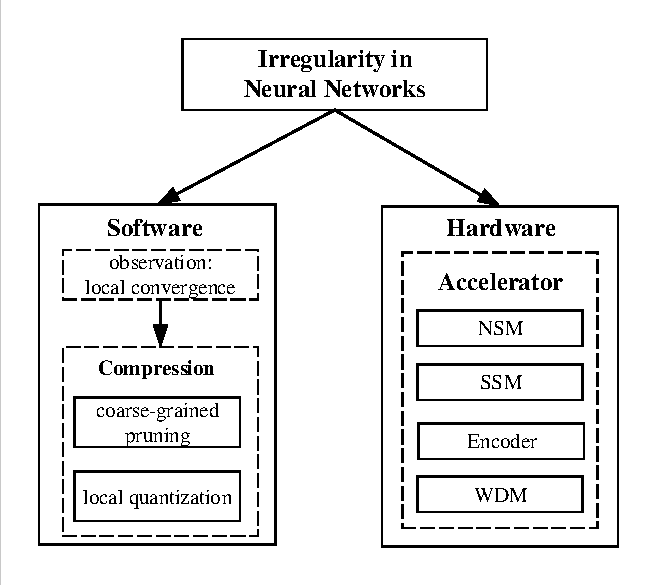
\includegraphics[width=0.8\columnwidth]{idea.pdf}
\caption{本文主要研究内容和创新点}
\label{fig:idea}
\end{figure}


最近的研究~\cite{han2015learning,han2015deep,wang2016cnnpack,zhou2017incremental}表明,神经网络可以在保持精度的前提下,通过稀疏,量化,低精度等方式进行深度压缩,从而减少参数存储量,计算量和访存量。然而,稀疏技术会使得原本规则的神经网络计算变得不规则,因此CPU,GPU以及一些不支持稀疏的加速器并不能从中受益。尽管,最近出现了一些能够支持稀疏的神经网络加速器~\cite{chen2017eyeriss,zhang2016cambricon,albericio2016cnvlutin,han2016eie,han2017ese,angshuman2017scnn},但是挖掘稀疏的效果并不理想,利用稀疏的效率也不高。

本文提出了一种软硬件结合方法(software/hardware cooprative approach)来处理稀疏神经网络的不规则性。我们首先提出了粗粒度剪枝算法,从而减少稀疏神经网络的不规则性,同时我们结合局部量化和熵编码对神经网络进行深度压缩。然后我们设计了粗粒度稀疏神经网络加速器Cambricon-S,来处理粗细度稀疏的神经网络,新型加速器有高性能和和低能耗的特点。本文的主要贡献如图~\ref{fig:idea}所示,可以归纳如下:

1.本文首次提出采用软硬件结合的方法处理稀疏神经网络不规则性。在软件方面我们提出了一种新的压缩算法对神经网络进行深度压缩,压缩算法中包含的粗粒度稀疏算法能够减少稀疏神经网络的不规则性;在硬件方面,我们提出了粗粒度稀疏神经网络加速器来Cambricon-S高效处理粗粒度稀疏,从而获得性能提升,同时降低能耗。

2. 本文观察到了局部收敛(local convergence)的现象,即在训练过程中,神经网络的权值不是一种随机分布的情况,大的权值会聚集成簇,我们通过大量实验证明局部收敛的现象出现在许多的神经网络中。本文根据观察到的局部收敛现象,提出了一种新的神经网络压缩算法。压缩算法包括三个步骤,分别是粗粒度剪枝(coarse-grained pruning),局部量化(local quantization)和熵编码(entropy coding)。粗粒度剪枝将神经网络的权值分为多个权值块,当一个权值块符合某个条件时将从网络拓扑中被完全剪除,粗粒度稀疏的神经网络对比与细粒度稀疏的神经网络拥有更低的不规则度。局部量化将权值分为多个子区域,然后在每一个子区域内分别进行量化,进一步压缩神经网络。之后,我们采用熵编码对神经网络进行无损压缩。新的神经网络算法不仅能够降低稀疏神经网络的稀疏度,还最终获得非常理想的压缩比。

3. 本文设计并提出了首个能够支持粗粒度稀疏神经网络的加速器微结构。该微结构不仅能够处理普通的稠密神经网络,还能够通过打开/关闭稀疏处理模块支持多种稀疏/量化情况,包括神经元稀疏,粗粒度权值稀疏,神经元/权值同时稀疏,局部量化等。新型加速器能够非常高效的利用稀疏和量化,获得非常理想的性能和能耗。

4. 本文针对神经网络加速器的计算特性,设计了专用的性能模拟器。该模拟器能够高速,精准地模拟神经网络在加速器的运行性能。

\section{论文的组织结构}
本文第一章介绍了本文的工作背景。我们主要从神经网络算法和神经网络加速器两方面介绍神经网络的发展简史,基本原理和面临的问题,在此基础上,我们提出了本文的主要研究内容和创新点。

本文第二章介绍了神经网络相关的背景知识。首先我们介绍了神经网络算法,对神经网络的多种不同类型的层计算进行详细分析。然后我们介绍了神经网络的低能耗技术,包括低精度计算技术和裁剪技术。最后我们介绍最新神经网络加速器的相关工作,其中我们重点介绍了稀疏神经网络加速器。

本文第三章提出了一种新的神经网络压缩方法。首先我们观察到神经网络的权值在训练过程中有局部收敛的现象,即大的权值容易聚集成簇。基于局部收敛,我们提出了粗粒度剪枝的策略,将多个权值同时进行裁剪操作;然后我们提出局部量化的方案进一步利用局部收敛,减少表示权值的比特数,进一步对神经网络进行压缩;最后我们利用熵编码对神经网络进行无损压缩。最后通过大量实验证明,新的压缩方法能够对神经网络进行深度压缩,同时减少稀疏神经网络的不规则性。

本文第四章提出了一个粗粒度稀疏神经网络加速器,能够快速处理经过深度压缩的神经网络。首先,我们观察粗粒度稀疏神经网络的特点,提出了设计加速器的三个原则。然后我们根据这三个设计原则,提出了新型加速器的架构,新的加速器能够充分利用神经元稀疏,粗粒度权值稀疏和局部量化,从而提高性能,降低功耗。最后我们为新型加速器设计了专用的编程框架,减轻用户的编程负担。

本文第五章提出了一个新型加速器专用的性能模拟器,我们根据新型加速器的特性,设计了一个性能模拟器代替周期精确模拟器,从而在误差允许的范围内,快速完成对加速器的性能评估。

本文第六章,我们对加速器进行详细的性能和能耗评估,在七个benchmark上,我们将Cambricon-S与CPU,GPU,DianNao和Cambricon-X进行性能和能耗的比较。最后我们根据实验结果详细分析了新型加速器能够获得高性能和低能耗的原因。

最后一章我们对本文进行总结,并展望了未来的研究工作。

\chapter{神经网络简介}

\citestyle{numbers}

\section{神经网络算法基础}
现代神经网络由多种不同类型的层组成,输入数据依次通过各个层被逐层处理,最终被分类,识别或者检测。在每一层中,神经元接收多个输入进行处理,然后通过连接将输出发送到下一层。神经元之间的连接,即所谓的突触,通常具有独立或者共享的权重。神经网络在图像处理,语音识别,语音合成,自然语言处理等领域有着非常广泛的应用。目前在图像处理应用最广泛的网络是卷积神经网络(convolutional neural networks,简称CNNs)和深度神经网络(deep neural networks,简称DNNs),它们由卷积层,池化层,归一化层,激活层和全连接层等组成。递归神经网络(recurrent neural networks,简称RNNs)是一类重要的机器学习技术,专门用于处理顺序数据序列和可变长度数据序列。RNNs在语音识别,自然语言处理,场景语义理解和时间序列分析等方面有着广泛的应用。其中应用最广泛,性能最高的两种类型的RNNs是长短时记忆网络(long short term memory,简称LSTM)和门控循环单元(gated recurrent unit,简称GRU)。下面将为大家介绍神经网络中集中常见的神经网络层类型。

\subsection{全连接层}
全连接层(fully connected layers)是神经网络算法中常见的一种层类型,主要用来将上一层提取的特征进行组合,综合以及分类,在整个神经网络中起到“分类器”的作用。全连接层的结构如图~\ref{fig:fc_layer}所示,输入层神经元为m个,输出层的神经元为n个,其中每一个输出神经元与所有输入神经元相连,其结构相当于n个m输入的感知机,因此全连接层也可以看成是感知机扩展。 
\begin{figure}
  \centering
  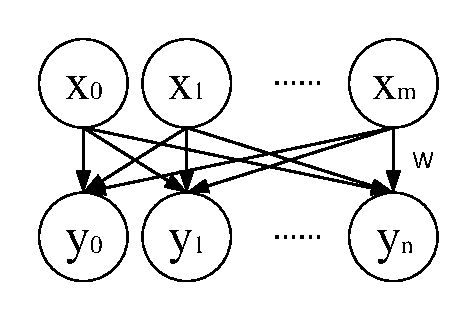
\includegraphics[width=0.5\columnwidth]{fc.pdf}
  \caption{\footnotesize 全连接层}
  \label{fig:fc_layer}
\end{figure}


全连接层的核心操作操作是矩阵向量乘积,
\begin{equation}
y=W*x+b
\end{equation}
其中$y$是输出神经元向量,$x$是输入神经元向量,$W$是权值矩阵,$b$是输出神经元的偏置向量。因此全连接层的本质是由一个特征空间线性变换到另一个特征空间,且目标空间的任一维都会收到源空间每一维的影响。由于每个输出神经元都要与输入神经元相连接,这样的话就会造成权值数量巨大,从而造成网络难以训练,并且会出现过拟合的情况。因此在CNN中,全连接层常出现在最后几层,用取于对前面设计提的特征做加权和。

\subsection{卷积层}
\begin{figure}[b]
  \centering
  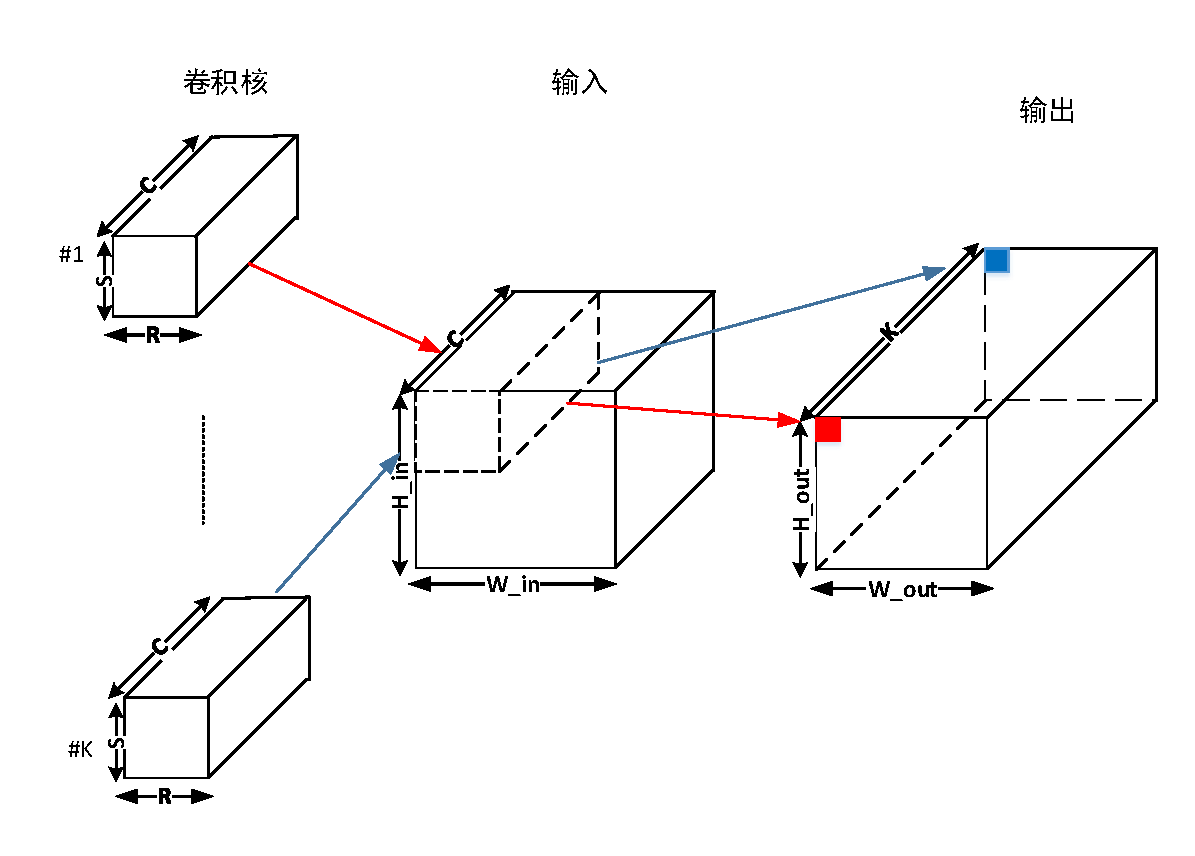
\includegraphics[width=0.8\columnwidth]{conv.pdf}
  \caption{\footnotesize 卷积层}
  \label{fig:conv_layer}
\end{figure}

卷积层(convolutional layers)是卷积神经网络的核心层,主要用于提取特征。卷积层受到生物学上感受野(Receptive Field)的机制而提出的。感受野主要是指听觉系统、本体感觉系统和视觉系统中神经元的一些性质。比如在视觉神经系统中,一个神经元的感受野是指视网膜上的特定区域,只有这个区域内的刺激才能够激活该神经元。在听觉系统中,对于语音则是某一时间戳后的时间段才能激活神经元。卷积层充分借鉴感受野的机制,神经元仅仅能够感受局部特征,而卷积核的大小直接限制感受野的大小,输出神经元只和周围一小块的输入神经元存在连接。局部连接的方法大大减少了卷积层中的权值数量。
卷积层采用了共享权值的方法进一步减少权值的数量,即同一输出特征图共享一组卷积核。同一个输出特征图像上的所有像素点是同一组卷积核在输入图像不同位置上提取到的图像特征,而这些图像特征具有相同意义。卷积层采用多组不同的卷积核对输入特征图进行卷积,从而获得多组输出特征图,即多组不同的图像特征。

卷积层的结构如图~\ref{fig:conv_layer}所示。卷积层的核心运算是二维滑动窗口卷积运算,即规模为$R\times S$的卷积核在规模为$W_{in}\times H_{in}$的输入特征图上滑动进行二维卷积,最终产生规模为$W_{out}\times H_{out}$的输出特征图。通常情况下,输入特征图不仅只有一个,而是由C个组成,即规模为$C\times W_{in}\times H_{in}$,因此我们对每个输入通道都施加一个卷积核,即使用规模为$C\times R\times S$的卷积核对输入进行卷积,最终获得一个输出特征图。当我们将采$K$组不同的卷积核作用于相同的输入特征图,将获得$K$个不同的输出特征图。最终,卷积层的输入规模为$C\times W_{in}\times H_{in}$,卷积核的规模为$K\times C\times R\times S$,输出规模为$K\times W_{out} \times W_{out}$。

\begin{lstlisting}[language=C, frame=single, basicstyle=\footnotesize, caption=六层卷积循环, label=list:convcode, captionpos=b]
for k=0 to K
    for w=0 to W
        for h=0 to H
            for c=0 to C
                for s=0 to S
                    for r=0 to R
                        out[k][w][h] += in[c][w*sw+r][h*sh+s] * filter[k][c][r][s]
\end{lstlisting}

卷积层的计算由K,C,R,S,W和H这六个变量形成嵌套循环完成,而且这六个变量的所有排列都是合法的。算法~\ref{list:convcode}展示了其中一种循环嵌套方式,我们可以用$N->W_{out}->H_{out}->C->S->R$来描述这种循环,其中$sw$和$sh$表示卷积操作的步长。不同的循环方式决定了数据的复用形式和数据流的方式,最终将影响神经网络加速器的设计~\cite{angshuman2017scnn}。

\subsection{池化层}
池化层(pooling layer)是神经网络中一个重要的层。池化层一般是在卷积层之后,对输入进行非线性降采样,常用的池化做法是对每个滤波器的输出求最大值,平均值,中位数等。
池化层的意义主要体现在两个方面:第一,池化层通过对特征图像进行降维操作,能够在保留显著特征的情况下,有效减少整个神经网络所需要的参数量和计算量。第二,池化层能够保证输入的平移不变性(translation invariant),这意味着即使图像的像素在邻域发生微小位移时,池化层的输出能够保持不变,从而增强神经网络的鲁棒性,由一定的抗扰动能力。常用的池化层包括最大池化层,平均池化层,ROI (Regions of interest)池化层.

最大池化层的基本思想是在一个特定的数据区域内选择一个最大值作为输出。其计算公式是
\begin{equation}
out_{x,y} = max(in_{x*sx,y*sy}:in_{x*sx+kx,y*sy+ky})
\end{equation}
其中$kx$和$ky$是池化窗口的大小,$sx$和$sy$是池化的步长。通常情况下池化窗口的大小与池化的步长相同,即池化操作的输入并不会重复。后来也出现了数据复用的池化,相邻池化窗口之间会有重叠区域,此时池化步长小于池化窗口的大小。


平均池化层的基本操作与最大池化层类似,它将一个特定的区域内的数据取算数平均作为输出,其计算公式是
\begin{equation}
out_{x,y}=mean(in_{x*sx,y*sy}:in_{x*sx+kx,y*sy+ky})
\end{equation}

ROI Pooling层主要是针对ROIs的池化操作,主要应用于物体检测领域的Fast RCNN和Faster RCNN网络中,它的特点是输入特征图尺寸不固定,但是输出特征图的尺寸固定。ROI Pooling的输入包含两部分,第一部分是特征图,在Fast RCNN中,它位于ROI Pooling之前;在Faster RCNN中,它是与RPN共享的那个特征图。第二部分是ROIS,在Fast RCNN中,指的是Selective Search的输出;在Faster RCNN中指的是RPN的输出,是一系列的矩阵候选框,每一个矩阵候选框用四个坐标和索引来表示。ROI Pooling的输出则是batch个三维向量($C \times W\times H$),其中batch的值为ROI的数量。因此ROI Pooling的过程可以总结为将大小不同的矩阵框映射为大小固定的矩阵框。
 

\subsection{归一化层}

\begin{figure}[b]
  \centering
  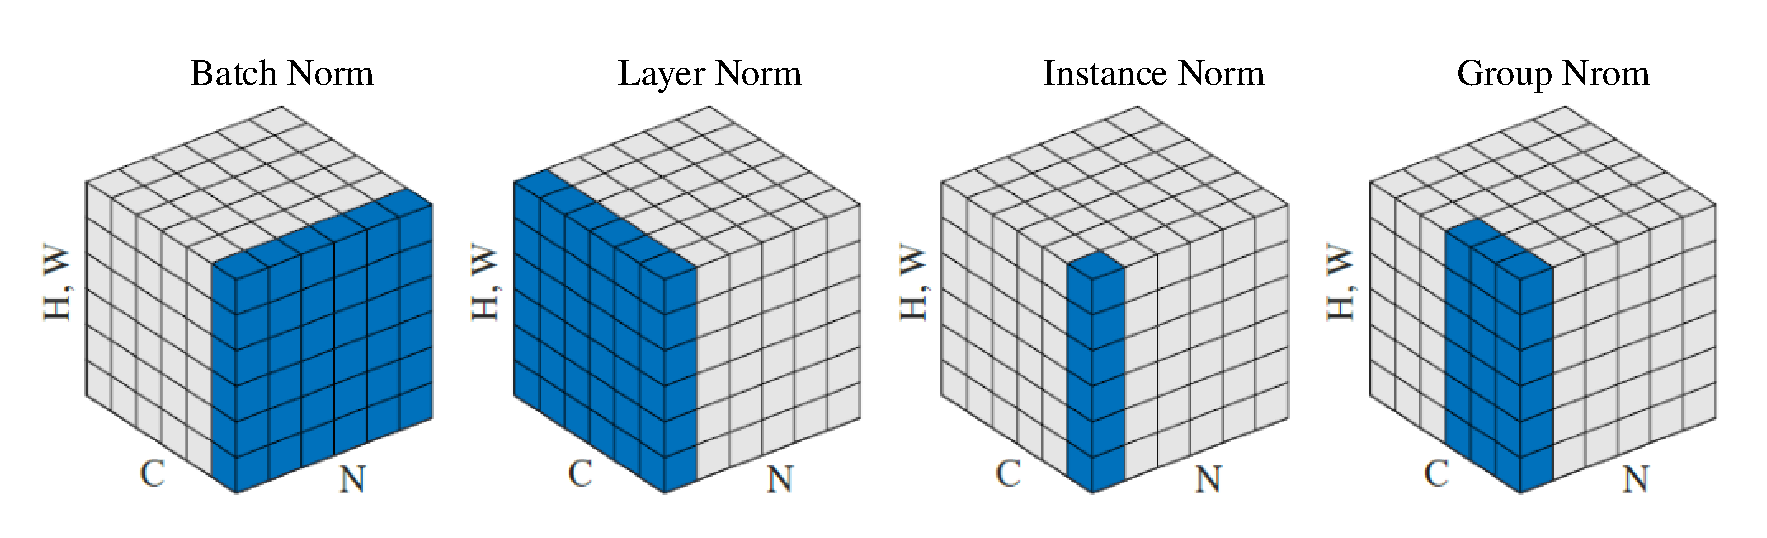
\includegraphics[width=1.0\columnwidth]{norm.pdf}
  \caption{\footnotesize 归一化方法。每一个子图显示的是一个feature map,其中N为batch轴,C为channel轴,(H,W)为空间轴。蓝色的像素表示归一化的范围。}
  \label{fig:norm}
\end{figure}

随着神经网络的规模不断变大,结构的复杂度增加,神经网络越来越难以训练,同时神经网络越来越容易出现过拟合的现象。归一化层(normalization layer)成为神经网络中不可或缺的一个层,它能够加快神经网络的收敛速度,防止过拟合,降低神经网络对初始化权重的敏感度,提高神经网络的精度。近几年出现了各种各样的归一化方法,主要包括LRN(Local Response Normalization)~\cite{krizhevsky2012imagenet},BN(Batch Normalization)~\cite{ioffe2015batch},LN(layer Normalization)~\cite{ba2016layer},IN(Instance Normalization)~\cite{dmitry2016instance}和GN(Group Normalization)~\cite{wu2018group}等。

LRN是AlexNet等网络中使用的归一化方法,它在每一个像素的小领域范围内进行归一化处理。目前主流的归一化方法则更加注重全局范围内的归一化处理,这些全局归一化的方法能够使得我们在训练神经网络时使用较大的学习率,从而加快神经网络训练速度。如图~\ref{fig:norm}所示,BN选择在batch维度上进行归一化处理;LN选择在channel维度进行归一化处理;IN执行类似BN的计算,但是仅仅在单个样本执行归一化;GN在IN的基础上对多个样本进行归一化。下面主要对BN的计算方法进行简要介绍。

BN的计算公式如下所示:
\begin{gather}
\mu _{\beta} = \frac{1}{N} \sum_{i=1}^{N} a_i \\
\theta _{\beta}^{2} = \frac{1}{N} \sum_{i=1}^{N}(a_i - \mu _{\beta})^{2} \\
\hat{a_i}=\frac{a_i - \mu _{\beta}}{\sqrt{\theta _{\beta}^2 + \epsilon}} \\
b_i = \gamma \hat{a_i} + \beta
\end{gather}

在上述算法中,$m$为batch数,$a_i$是第i个batch的输入数据,$\mu _{\beta}$ 和 $\theta _{\beta}^{2}$分别是N个输入的均值和方差,参数$\epsilon$是批变化常量,参数$\gamma$和$\beta$是训练时需要学习的参数,$b_i$是最后归一化后的输出。

\subsection{激活层}
激活层(activation layer)是神经网络能够解决非线性问题的关键,它弥补了神经网络中线性模型表达能力不足。目前主流的激活函数包括Sigmoid, Tanh, ReLU以及ReLU的变种,如PReLU和RReLU等。

Sigmoid,Tanh和ReLU的函数图如图x所示,公式分别为
\begin{gather}
Sigmoid(x) = \frac{1}{1 + \eu^{-x}} \\
Tanh(x) = \frac{1-\eu^{-2x}}{1+\eu^{-2x}} \\
ReLU(x)=
\begin{cases}
x & \text{if } x > 0, \\
0 & \text{if } x \leq 0
\end{cases}
\end{gather}

Sigmoid函数主要被应用于早期的神经网络中,Sigmoid函数拥有良好的性质,Sigmoid函数的值域范围限制在(0,1)之间,这与概率值的范围是相对应的,这样sigmoid函数就能与一个概率分布联系起来了;同时Sigmoid函数的导数可以由其本身求得$Sigmoid(x)^{'}=Sigmoid(x)(1-Sigmoid(x))$。但是Sigmoid函数也有不少缺点,首先Sigmoid函数的输出并不是以0为中心,这个特性会导致为在后面神经网络的高层处理中收到不是零中心的数据,进而训练时的权值更新产生锯齿晃动。同时Sigmoid函数具有饱和性,容易出现梯度消失的现象,使得神经网络难以训练。

Tanh函数是Sigmoid函数的改进版本,它的收敛速度比Sigmoid函数更快,相比Sigmoid函数,其输出以0为中心,但是仍然存在饱和性而导致梯度消失的问题的。Tanh函数和Sigmoid函数目前主要被用于基于LSTM的RNN架构或者基于GRU的RNN架构中。

ReLU是目前非常流行的激活函数,它是分段线性函数,所有的负值为0,而正值不变,这种操作被称为单侧抑制。单侧抑制使得神经网络中的神经元也具有了稀疏激活性,尤其体现在深度神经网络模型(如CNN)中,当模型增加N层之后,理论上ReLU神经元的激活率将降低2的N次方倍,从而更好地挖掘相关特征,拟合训练数据。同时,ReLU不存在饱和区,因此不存在梯度消失的问题,使得模型的收敛速度维持在一个稳定的状态。\cite{krizhevsky2012imagenet}实验显示ReLU单元比tanh单元具有6倍的收敛速度提升。

\subsection{LSTM}

\begin{figure}[b]
  \centering
  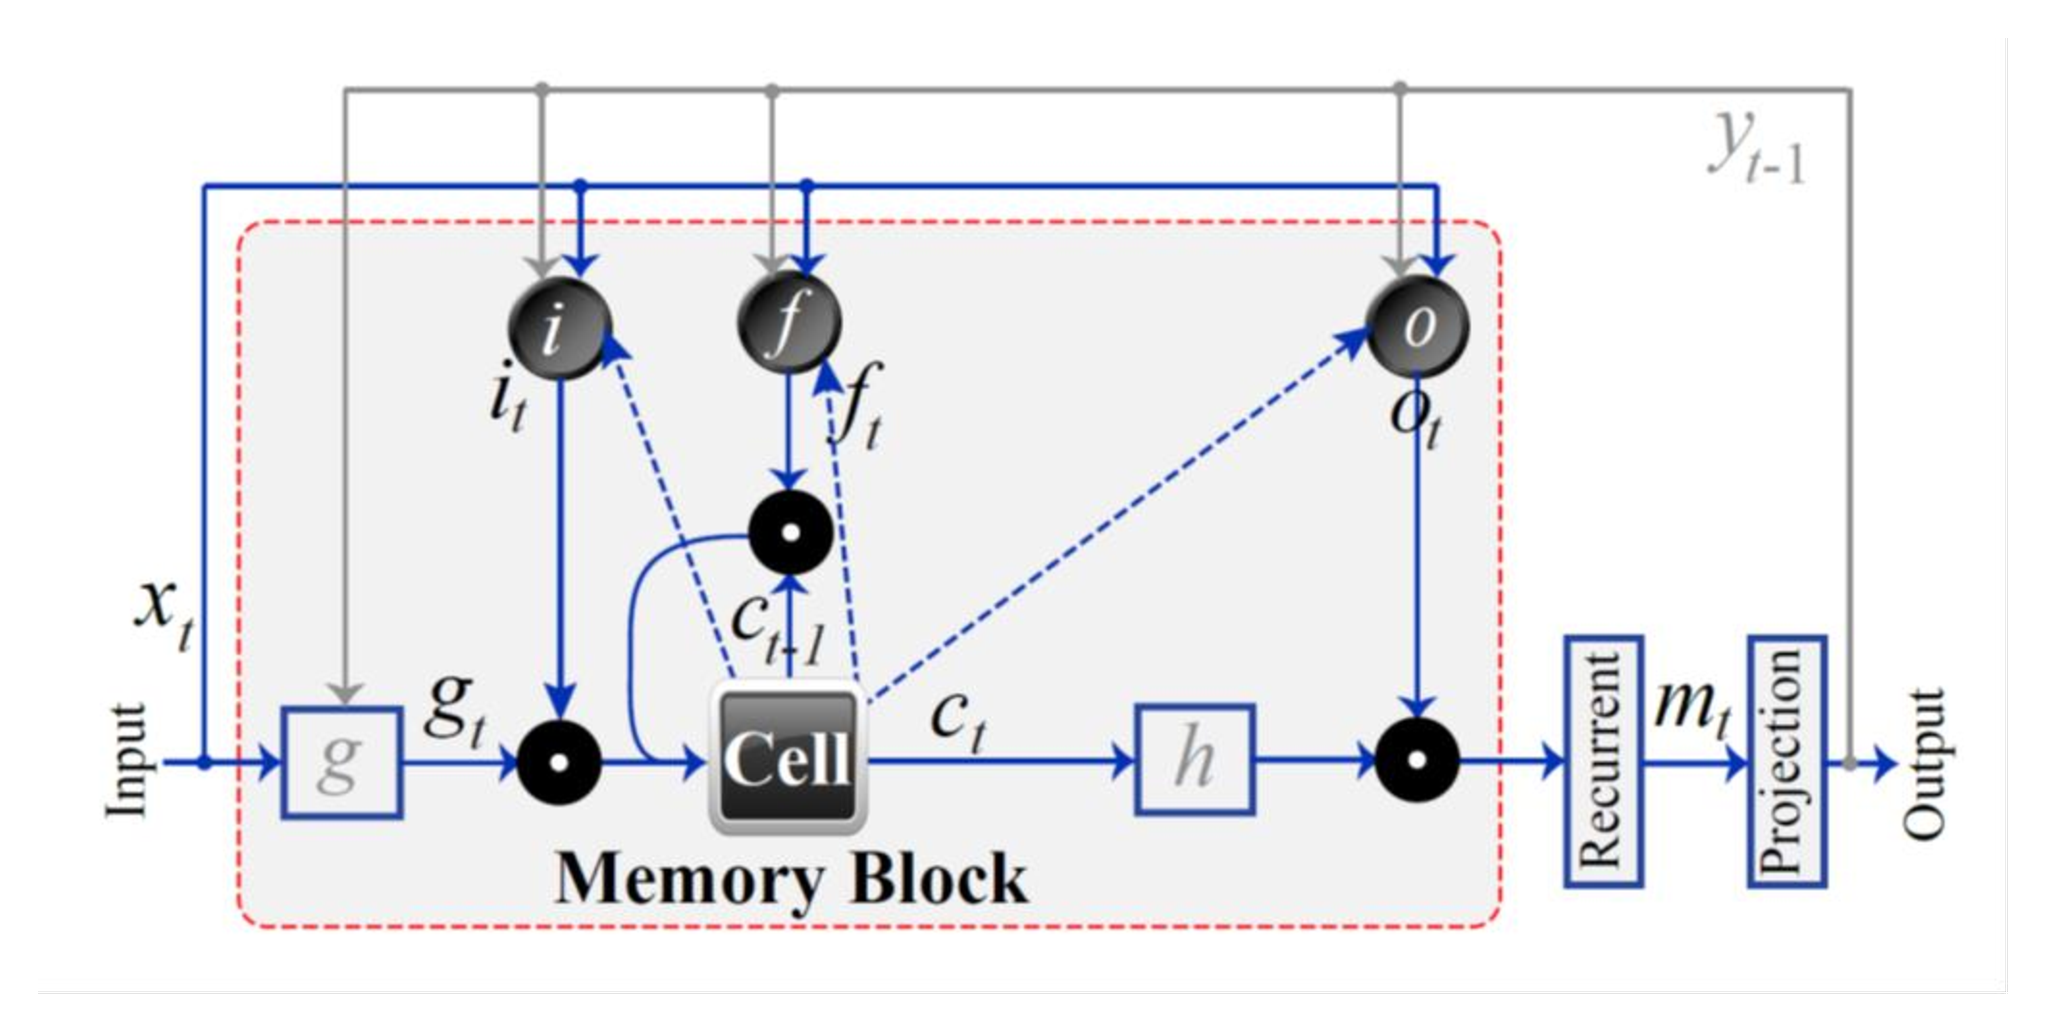
\includegraphics[width=0.7\columnwidth]{lstm.pdf}
  \caption{\footnotesize 一个基于LSTM的RNN架构.}
  \label{fig:lstm}
\end{figure}

\begin{figure}[h]
\centering
\begin{minipage}[b]{0.45\columnwidth}
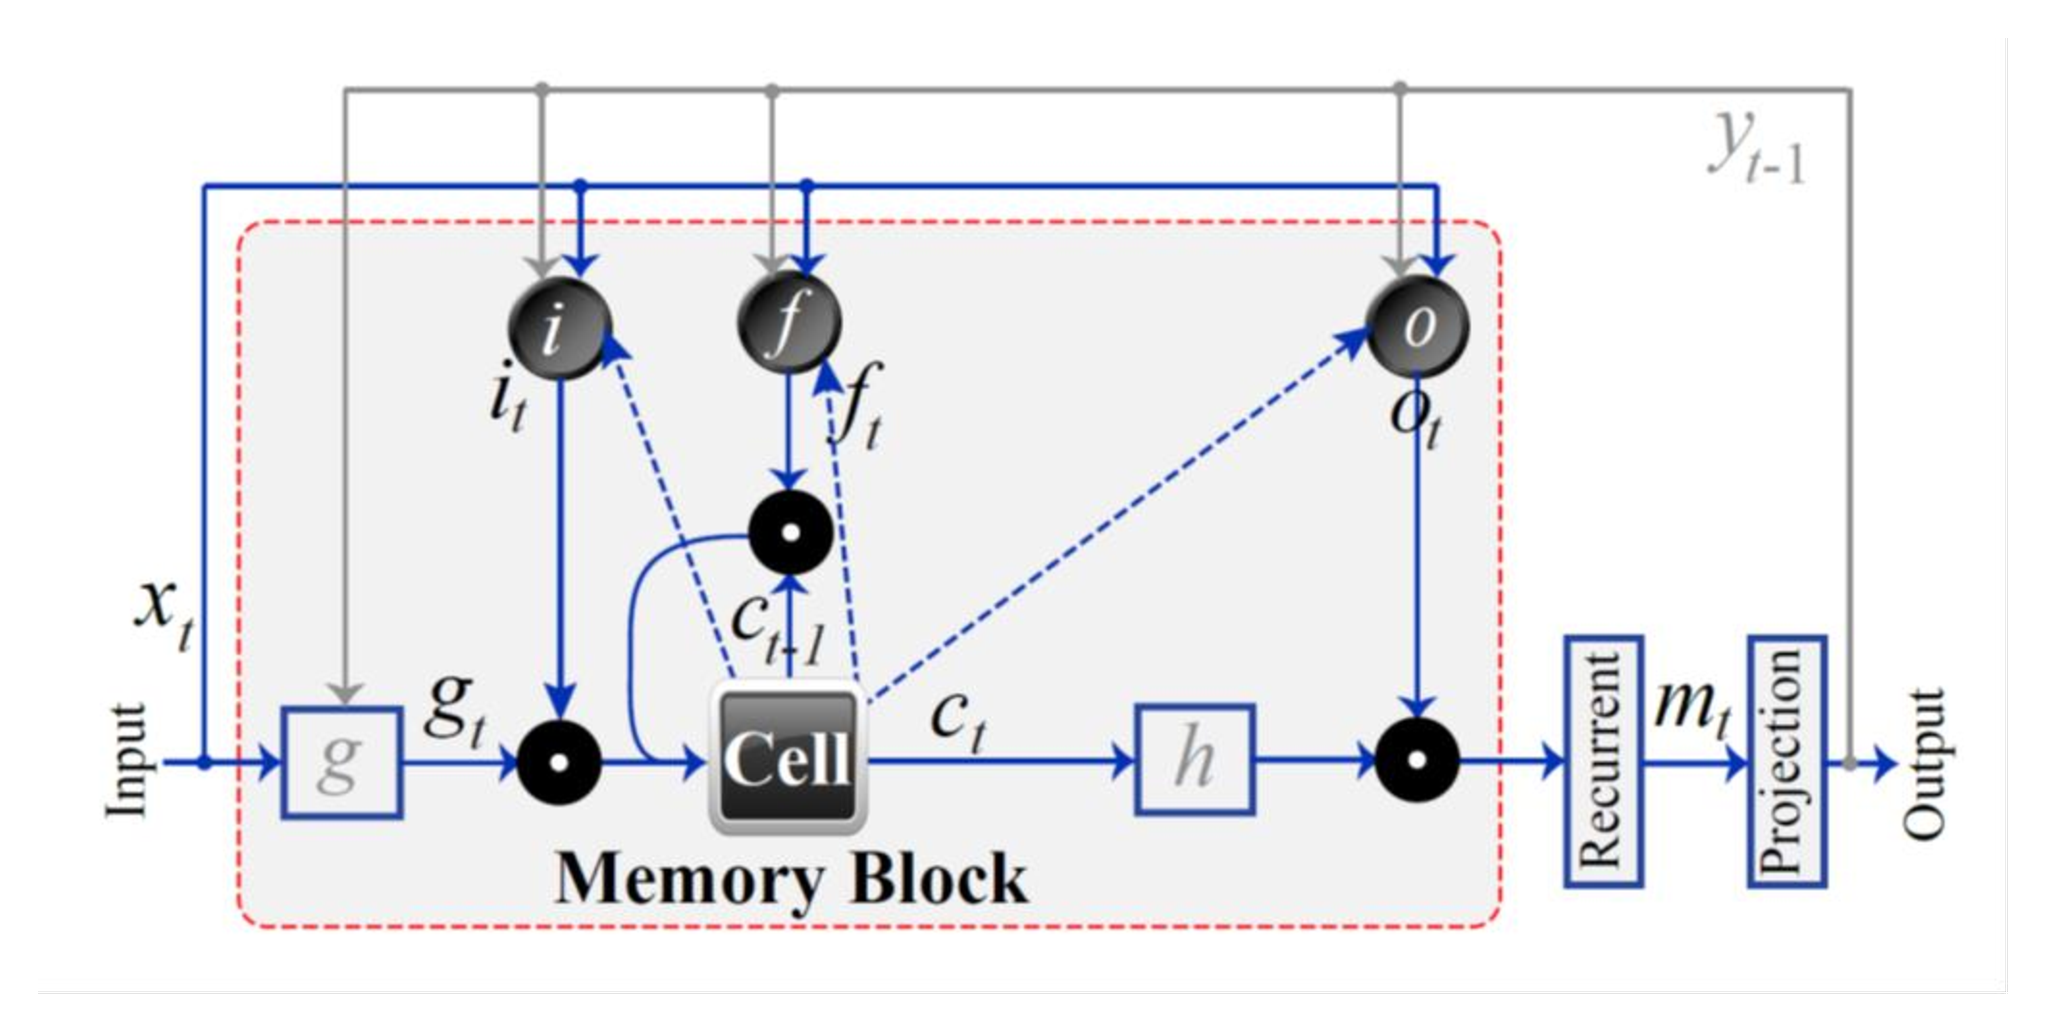
\includegraphics[width=\columnwidth]{lstm.pdf}
\end{minipage}
\hfill
\begin{minipage}[b]{0.45\columnwidth}
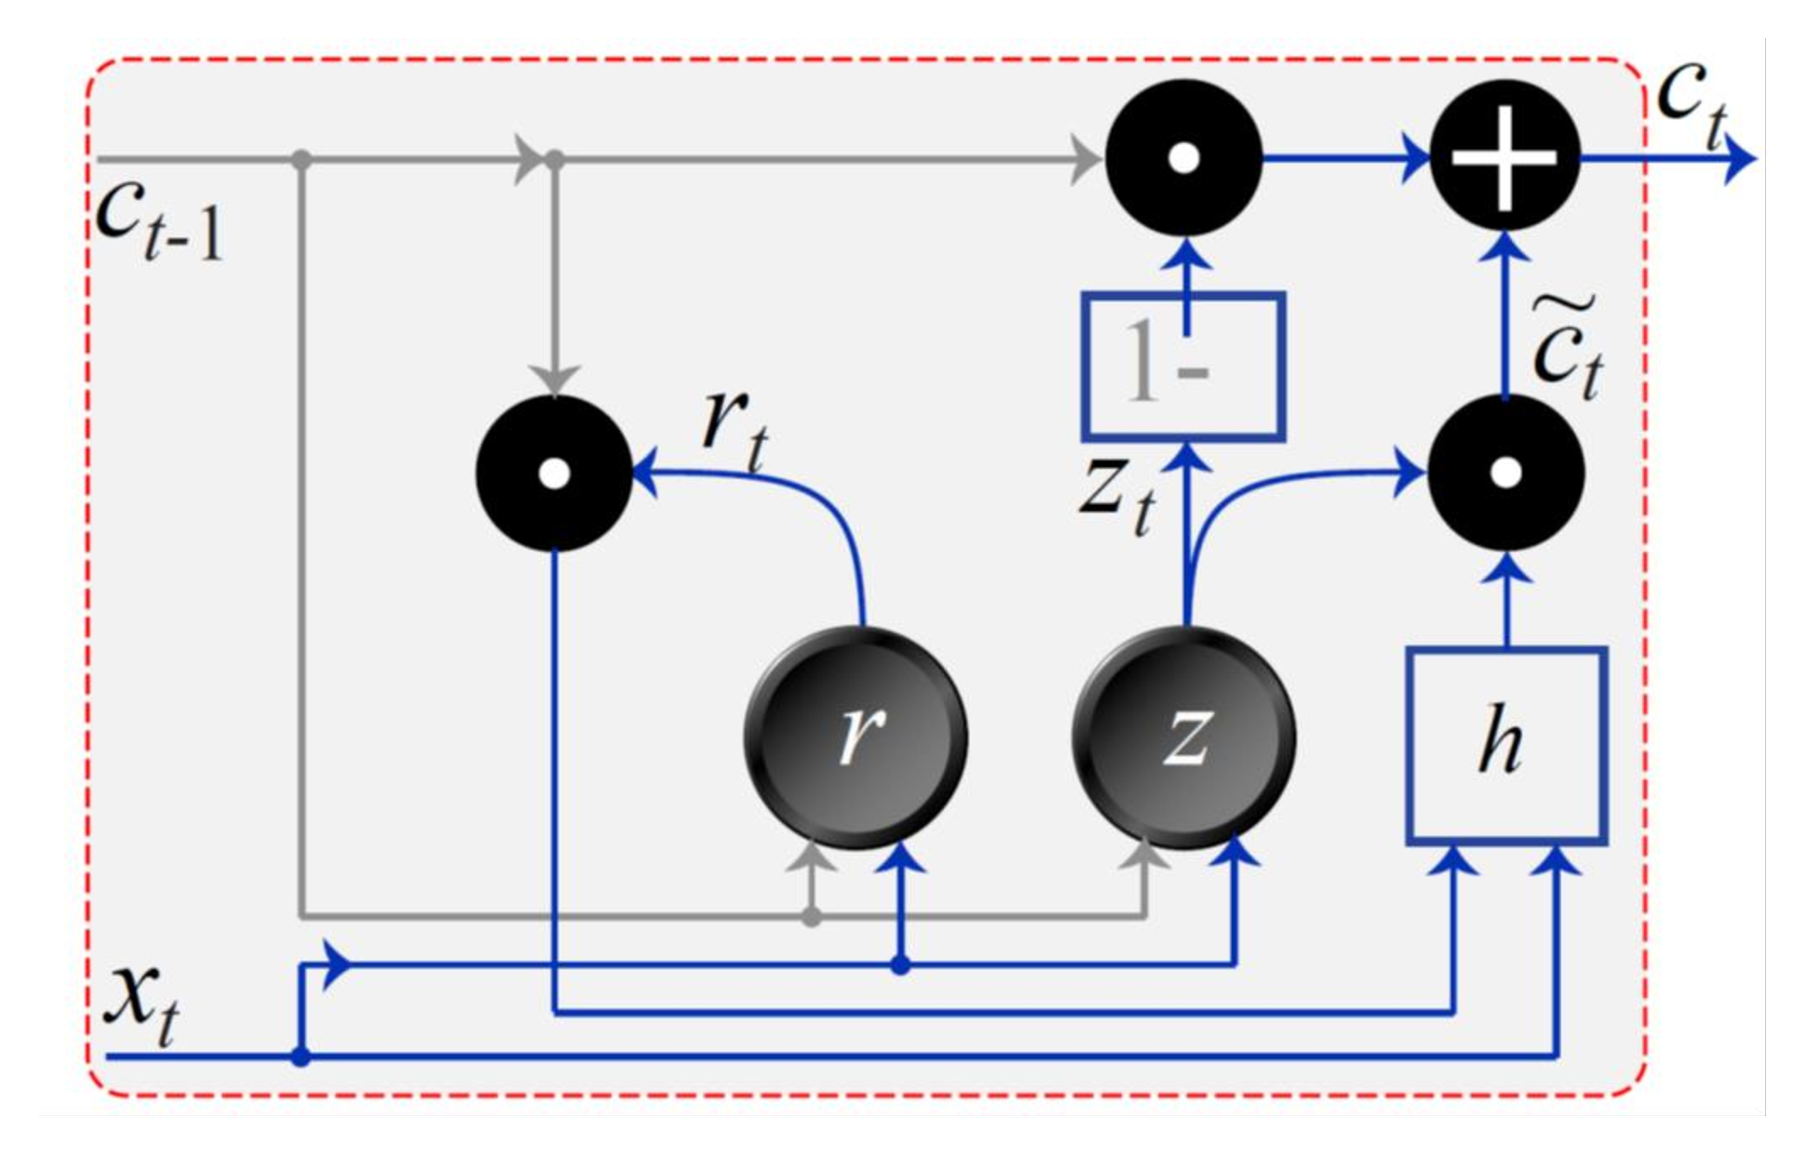
\includegraphics[width=\columnwidth]{gru.pdf}
\end{minipage}
\caption{\footnotesize (a) LSTM (b) A sparse MLP.}
\label{fig:RNN}
\end{figure}

现代大规模自动语音识别(automatic speech recognition,简称ASR)系统利用基于LSTM的RNN作为其声学模型。LSTM模型由一系列大规模矩阵组成,这是ASR的所有步骤中计算量最大的部分。在基于LSTM的RNN中,时刻T的输入取决于时刻T-1的输出。
一个经典的LSTM模型如图~\ref{fig:lstm}所示。
LSTM模型包含特殊存储单元(图~\ref{fig:lstm}中的$cell$)和三个特殊的门(图~\ref{fig:lstm}中的$i$,$o$,$f$),其中$cell$用于存储网络的时间状态信息,门用于执行特殊的乘法运算,包括输入门(input gate)、输出门(output gate)和遗忘门(forget gate)。输入门$i$控制输入到存储单元中的输入量;输出门$o$控制输出值;遗忘门$f$自适应地遗忘$cell$中存储的信息,从而控制前一状态对现状态的影响。除了基本的三个众所周知的门和$cell$之外,该LSTM模型还引入了窥视孔(peephole)和投影层(projection layer),以便更好地学习。窥视孔将缩放后的$cell$状态添加到三个门,其中缩放尺度由三个对角矩阵决定。投影层线性地将输出转换为低维形式。

LSTM模型的接收一个输入序列$X=(x_1;x_2;x_3;...;x_T)$(其中$x_t$是t时刻的输入向量)和上一个状态的输出序列$Y^{T-1}=(y_0;y_1;y_2;...;y_{T-1})i$(其中$y_{t-1}$是t-1时刻的输出向量)。利用下列公式从t=1到T计算输出序列$Y=(y1;y2;y3;...;y_T)$:
\begin{gather}
i_t=\delta (W_{ix}x_t + W_{ir}y_{t-1} + W_{ic}c_{t-1} + b_i), \\
i_t=\delta (W_{ix}x_t + W_{ir}y_{t-1} + W_{ic}c_{t-1} + b_i), \\
f_t=\delta (W_{fx}x_t + W_{fr}y_{t-1} + W_{fc}c_{t-1} + b_f), \\
g_t=\delta (W_{cx}x_t + W_{cr}y_{t-1} + b_c), \\
c_t=f_t \odot c_{t-1} + g_t \odot i_t, \\
o_t=\delta (W_{ox}x_t + W_{or}y_{t-1} + W_{oc}c_{t} + b_o), \\
m_t=o_t \odot h(c_t), \\
y_t=W_{ym}m_t 
\end{gather}

其中符号$i$、$f$、$o$、$c$、$m$和$y$分别是输入门、遗忘门、输出门、$cell$状态、$cell$输出和投影输出;$\odot$表示向量逐元素乘积,$W$表示权值矩阵(例如$W_ix$是从输入向量$X_t$到输入门的权值矩阵),$b$表示偏置向量。值得注意的是$W_ic$、$W_fc$和$W_oc$是用于peephole连接的对角矩阵,因此它们本质上是向量。$\delta$是Sigmoid激活函数,$h$是用户自定义的激活函数,通常情况下会采用$tanh$激活函数。

\subsection{GRU}
\begin{figure}[b]
  \centering
  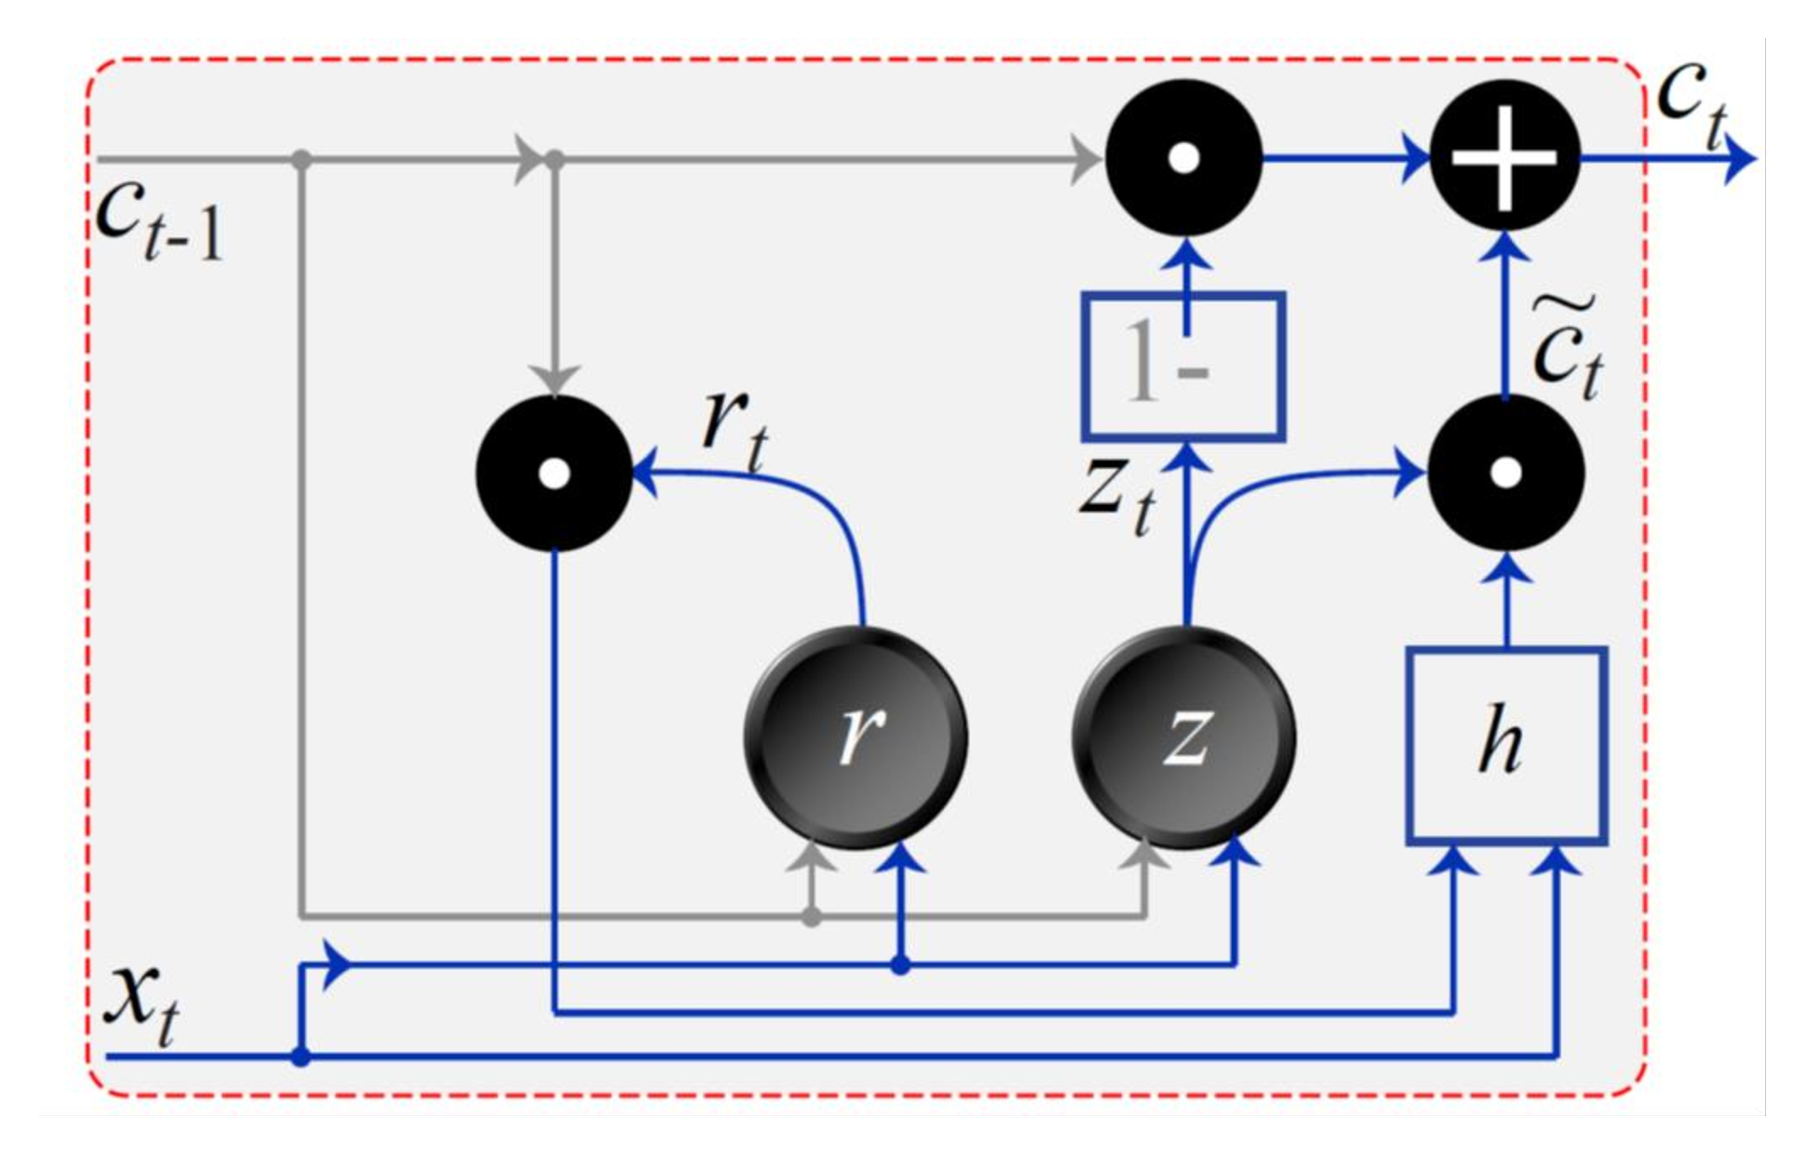
\includegraphics[width=0.7\columnwidth]{gru.pdf}
  \caption{\footnotesize 一个基于GRU的RNN架构.}
  \label{fig:gru}
\end{figure}
GRU是LSTM的变体,它把遗忘门和输入门组合成一个更新门(update gate)。它还合并了$cell$状态和隐藏状态,并进行了一些其他更改。GRU架构如图~\ref{fig:gru}所示。类似地,它遵循如下的公式从t=1到T进行迭代计算:
\begin{gather}
z_t=\delta(W_{zx}x_t+W_{zc}c_{t-1}+b_z),\\
r_t=\delta(W_{rx}x_t+W_{rc}c_{t-1}+b_r),\\
\tilde{c_t}=h(W_{\tilde{c}x}x_t+W_{\tilde{c}c}(r_t \odot c_{t-1}) + b_{\tilde{c}}),\\
c_t=(1-z_t) \odot c_{t-1} + z_t \odot \tilde{c_t}
\end{gather}
其中符号$z$、$r$、$\tilde{c}$、$c$分别是更新门、复位门、复位状态和$cell$状态;$\odot$表示逐元素乘法。$W$表示权值矩阵,$\delta$是Sigmoid激活函数,$h$是用户定义的激活函数,这里我们使用$tanh$激活函数。值得注意的是GRU有两个门(更新门和复位门),而LSTM有三个门(输入门、遗忘门、输出门),GRU中不存在LSTM中存在的输出门,而是将$cell$状态作为输出。LSTM中输入门和遗忘门耦合称为GRU中的更新门$z$,复位门$r$直接作用于到上一个$cell$的状态。 


\section{神经网络低能耗的技术}
随着神经网络算法被应用于更复杂的处理任务和更广泛的场景中,神经网络的规模也越来越大。最新的DNNs~\cite{le2013building, coates2013deep}需要数百兆字节甚至千兆字节来存储神经元和权值;同时需要数十亿次的乘加操作完成运算。考虑未来神经网络将朝着规模更大,层数更深的趋势发展,未来的大规模网络很难部署到嵌入式系统中。因此很多研究人员致力于减少神经网络的参数规模,从而减少存储资源,运算资源和带宽需求,提升性能同时降低能耗。目前已经有了一些有效的算法来解决这个问题,主要方法包括神经网络的低精度计算和神经网络压缩模型。

\subsection{神经网络的低精度计算}

最近研究~\cite{gupta2015deep}表明,在深度神经网络的训练中,不需要全精度的数据。使用低比特的权值表示,可以显著减少网络存储需求和运算能耗,特别是当使用极低比特位,如二进制/三元权值时。研究显示,非精确的计算(在神经元和权重中加入噪音)具有正则化的效果,从而减少泛化误差~\cite{goodfellow2016deep}。~\citet{gupta2015deep}使用16位定点数字表示来训练网络。~\citet{koster2017flexpoint}提出了动态数据格式(FlexPoint),用来完全替代32位浮点格式。Flexpoint具有一个可动态调整的共享指数,以最小化溢出和最大化可用动态范围。在训练过程中,数据范围会随着训练轮数的增长而连续变化,其中共享指数部分可以根据历史数据进行预测。实验结果显示,采用16位尾数和5位共享指数的Flexpoint格式数据在训练神经网络时,能够获得32位浮点类似的精度,并且远远超过16位浮点获得的精度。~\citet{dettmers20158}使用8比特量化神经网络,在保持性能的情况下,加快神经网络训练速度。在~\cite{courbariaux2015binaryconnect}和~\cite{hu2018hashing}中,作者表明,深度神经网络可以通过二进制权值进行训练,在某些情况下,它的精度可能超过使用浮点数进行训练的结果。~\citet{rastegari2016xnor}首先提出了三元权值网络 (Ternary Weight Network, TWN), 并在ImageNet~\cite{russakovsky2015imagenet}数据集上取得良好的效果。三元权值网络在~\cite{li2016ternary,zhu2016trained}等工作中被不断深入研究,其中~\cite{zhu2016trained}提出了学习三元值和三元赋值的方法。~\citet{zhou2017incremental}提出了INQ (Incremental Network Quantization),在不降低网络精度的情况下,将神经网络的权值量化为$2^{-n}$的形式。~\citet{wang2017fixed}提出了定点分解网络 (Fixed-point Factorized Network, FFN),使用定点分解的方式对神经网络权值进行三元化。这些方法可以在ImageNet上达到与全精度相当的精度,但是,这些工作只对权值进行量化,而使激活保持浮点格式。

除了对神经网络权值进行量化外,也有许多研究对激活进行量化。通过将权重和激活转换为低比特格式,网络计算需要使用定点操作,从而更有效地节约资源。~\citet{hubara2016binarized}中提出的二值神经网络 (binarized neural network, BNN),在CIFAR-10这样的小数据集上达到了跟浮点数类似的精度。~\citet{rastegari2016xnor}提出了另一个名为xnorn-net的网络,该网络将权值和激活都进行了二值化,在像ImageNet这样的大数据集上,xnor-net比BNN更精确,但是,它的精度对比浮点数的情况仍然有很大的下降。~\citet{zhou2016dorefa}提出了doref-net,研究了量化时比特位长度对权值、激活和梯度的影响。~\citet{cai2017deep}提出了HWGQ (Half-wave Gaussian Quantization) 的方法对权值和激活同时进行量化。与权值量化相比,激活量化通常会导致更大幅度的精度下降。对AlexNet和VGG16这样的大型网络进行量化,这些方法会导致精确度下降$5\%  ~ 10\%$。因此,如何用低比特位来量化权值和激活仍然是一个具有挑战性的问题。


\subsection{神经网络压缩模型}
大规模的神经网络通常是过拟合的,过多的参数会严重影响神经网络的运算速度。因此,我们可以通过压缩神经网络模型的方式来缓解过拟合的情况,同时减少神经网络的存储需求和运算需求。神经网络压缩的方法可以分为两类,剪枝和矩阵分解。

\citet{han2015learning}提出了剪枝的策略来减少神经网络中权值的数量,在不影响神经网络准确性的前提下,能够将神经网络所需要的存储量和计算量减少一个数量级。剪枝策略首先对神经网络进行训练,找出那些重要的连接;接下来,修剪那些不必要的连接;最后对神经网络进行冲训练,微调剩余连接的权值。实验显示,剪枝策略能够将AlexNet网络的权值数量减少9倍,将VGG16网络的权值数量减少13倍。

在此基础上,~\citet{han2016eie}进一步提出了Deep Compression用来深度压缩神经网络。Deep Comression由三个阶段组成:剪枝(Pruning),量化(quantization)和霍夫曼编码(Huffman Coding),最终在不影响神经网络的精度的前提下将神经网络压缩了35倍到49倍。Deep Compression首先通过剪枝阶段学习网络中重要的连接,删除不必要的连接,这个步骤能够减少9倍到13倍的权值。然后通过聚类算法将权值进行聚类,然后量化权值实现权值的共享,这个步骤能够减少表示每个权值的比特数,从32比特减少到到5比特。最后采用霍夫曼编码进一步无损压缩神经网络,这个步骤能够节省$20\%~30\%$的网络存储开销。在ImageNet数据集上,Deep Compression能够将AlexNet网络压缩35倍,将网络规模从$240MB$压缩到$6.9MB$。同时,Deep Compression将VGG16网络压缩了49倍,将网络规模从552MB压缩到11.3MB。这将允许我们将网络模型存储在加速器的片上SRAM缓存中,而不需要在片上和片外之间反复搬运权值,从而减少片外访存开销。

\citet{wang2016cnnpack}提出了一种新的有效的CNN压缩方法CNNpack,它在频域对神经网络进行剪枝操作,因此它不仅能够关注小的权值,同时关注所有潜在的对计算结果影响小的连接。CNNpack借助离散余弦变换(Discrete Cosine Transform,DCT)将空间域的权值变换到频域,然后采用聚类的方法将频域中的权重分解为公共部分和私有部分(残差)。在这两部分中,采用剪枝的策略丢弃大量的低能级的频率系数,能够在不显著降低精度的情况下产生高压缩比。在此基础上,CNNpack接着采用量化,霍夫曼编码和CSR存储的方法进一步压缩神经网络。最终实验实验显示,CNNpack能够对AlexNet和VGG16分别压缩35倍和49倍。

除了以上对权值进行剪枝的策略,还有不少研究工作直接对神经元进行剪枝操作~\cite{he2014reshaping,srinivas2015data,hu2016network,mariet2015diversity}。但是对神经元直接进行剪枝操作会严重降低神经网络的精度,因此不能获得很低的稀疏度。Data-free Parameter Pruning~\cite{srinivas2015data}在AlexNet和LeNet5上仅仅能够获得$65.11\%$和$16.5\%$的稀疏度,远远高于权值剪枝策略~\cite{han2015learning}的$11\%$和$8\%$。Network Trimming~\cite{hu2016network}能够在VGG16和LeNet5上获得$37\%$和$26\%$的系数率,也高于~\cite{han2015learning}中的$7.5\%$和$8\%$。

除了经典的剪枝策略(包括权值剪枝和神经元剪枝),还有一部分的研究工作基于矩阵分解和因式分解~\cite{denton2014exploiting,jaderberg2014speeding,lebedev2014speeding},这些方法可以保持原始模型的规则密集计算结构,在通用处理器上实现神经网络压缩和加速。~\citet{denton2014exploiting}是利用神经网路线性结构的特性,对神经网络进行适当的低秩分解(low-rank approximation),在精度损失在$1\%$的情况下,在很多模型上都能获得超过2倍的加速。~\citet{jaderberg2014speeding}利用将$k\times k$的卷积核分解为$k\times 1$和$1\times k$的卷积核,从而加速卷积计算。同时~\cite{jaderberg2014speeding}提出了两种优化方案:一种是利用滤波重构的方法最小化滤波权值误差,另一种是利用数据重构最小化响应误差的。~\citet{lebedev2014speeding}则采用CP decomposition的方式对大规模神经网络的卷积核进行分解和加速,实验结果显示,在精度损失低于$1\%$的情况下,在AlexNet网络能够获得4倍的加速效果。



\section{神经网络加速器}
\begin{table}[b]
  \footnotesize
  %\small
  \centering
\caption{\footnotesize 现有神经网络加速器的数据流形式}
\label{tab:dataflow}
\begin{tabular}{@{}lllll@{}llllllll}
  \toprule
  数据流 & 加速器\\
  \midrule
  基于向量算子的数据流 & DianNao~\cite{chen2014diannao}, DaDianNao~\cite{chen2014dadiannao}, PuDianNao~\cite{liu2015pudiannao}, Cambricon~\cite{liu2016cambricon}, \\ 
  ~ & Cambricon-X~\cite{zhang2016cambricon}, Cnvlutin~\cite{albericio2016cnvlutin}, EIE~\cite{han2016eie}, ESE~\cite{han2017ese} \\
  基于乘加算子的空间数据流 & ShiDianNao~\cite{du2015shidiannao}, Eyeriss~\cite{chen2017eyeriss}, TPU~\cite{jouppi2017tpu}, Neuflow~\cite{farabet2011neuflow} \\
  ~& SCNN~\cite{angshuman2017scnn}  \\
\bottomrule
\end{tabular}
\end{table}

\begin{figure}[t]
  \centering
  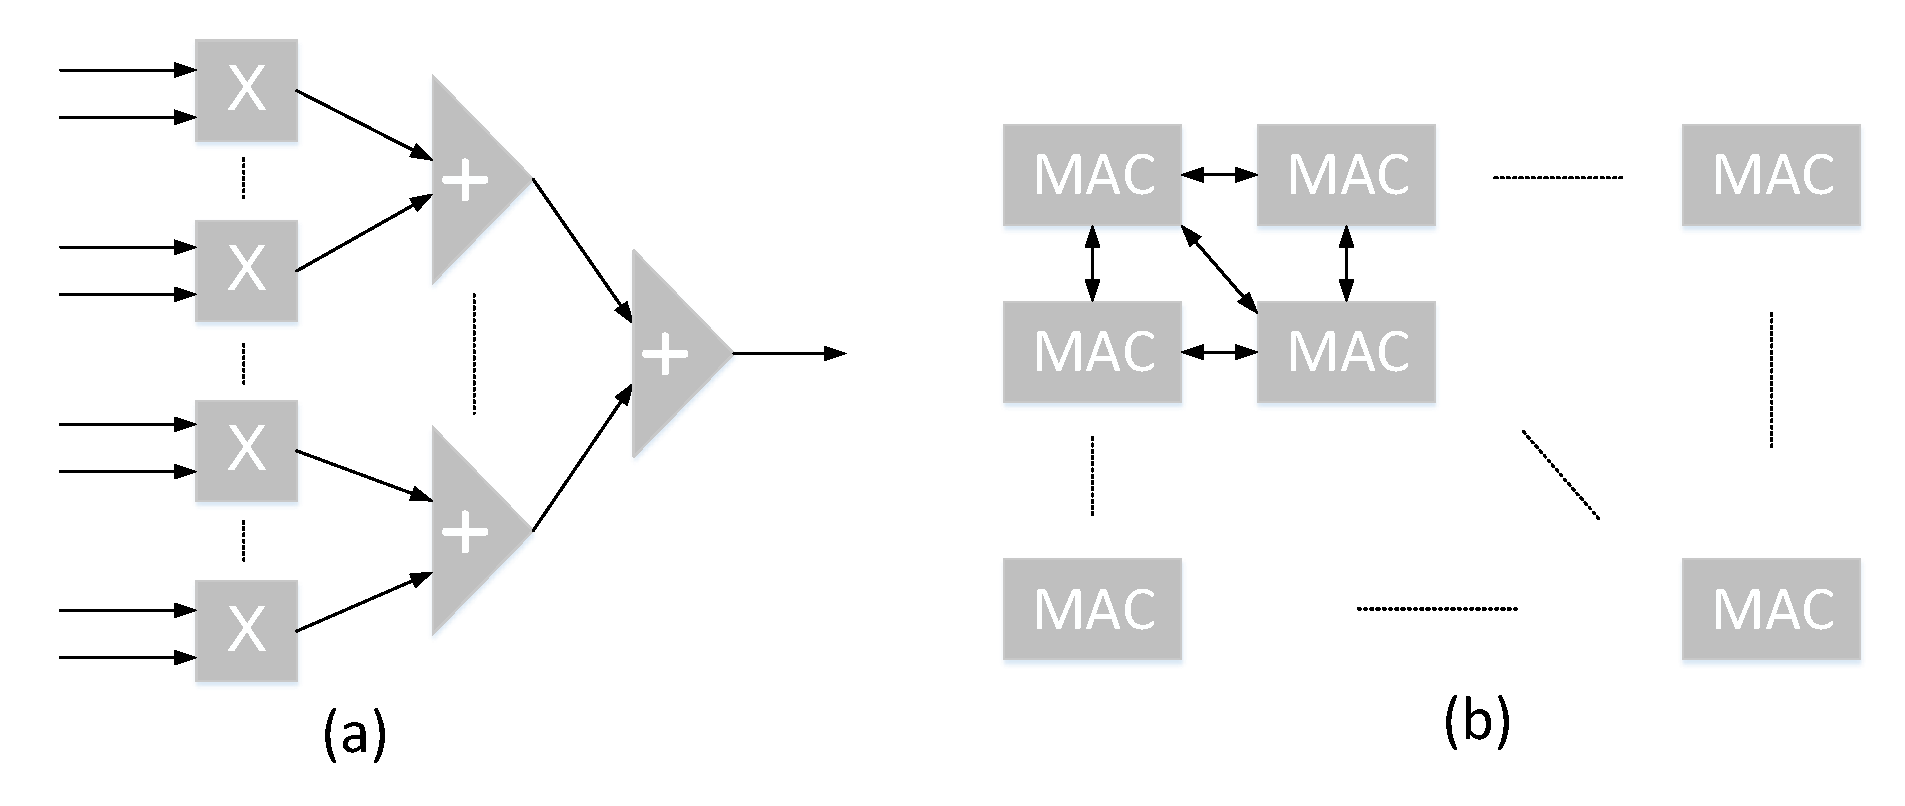
\includegraphics[width=0.7\columnwidth]{dataflow.pdf}
  \caption{\footnotesize 现有的加速器架构.}
  \label{fig:dataflow}
\end{figure}

\subsection{现有神经网络加速器架构}
由于严峻的能耗约束和高性能要求,定制加速器成为CPU和GPU等传统处理平台的替代品。近几年出现了数据流和结构各异的神经网络加速器。神经网络加速器按照数据流的形式可以分为两类,分别是基于向量算子数据流的加速器和和基于乘加算子(multiply-and-accumulate,简称MAC)空间数据流的加速器。基于向量算子的加速器将神经网络的运算转化为向量运算,主要是将矩阵操作转化为一系列的向量操作(通常是内积操作)。如图~\ref{fig:dataflow} (a) 所示的结构中,n个乘法器和一个n输入的加法树就能够完成两个n维向量的内积操作。基于乘加算子的加速器(如图~\ref{fig:dataflow}(b))通常具有一系列的规则分布的处理单元,其中每一个处理单元能够完成一次MAC操作。处理单元之间采用一种规律的方式进行连接(如二维矩阵),神经元和权值采用某种规律的方式在处理单元之间进行移动,如经典的脉动阵列形式(systolic design),因此这种形式又称为空间数据流形式。表~\ref{tab:dataflow}总结了近年来出现的神经网络加速器和它们的数据流形式。
基于向量算子的神经网络加速器包括DianNao~\cite{chen2014diannao},DaDianNao~\cite{chen2014dadiannao},PuDianNao~\cite{liu2015pudiannao},Cambricon~\cite{liu2016cambricon},Cambricon-X~\cite{zhang2016cambricon},Cnvlutin~\cite{albericio2016cnvlutin}, EIE~\cite{han2016eie}和ESE~\cite{han2017ese}。基于乘加算子空间数据流的加速器包括ShiDianNao~\cite{du2015shidiannao}, Eyeriss~\cite{chen2017eyeriss}, TPU~\cite{jouppi2017tpu}, Neuflow~\cite{farabet2011neuflow}和SCNN~\cite{angshuman2017scnn}。


\begin{figure}[t]
  \centering
  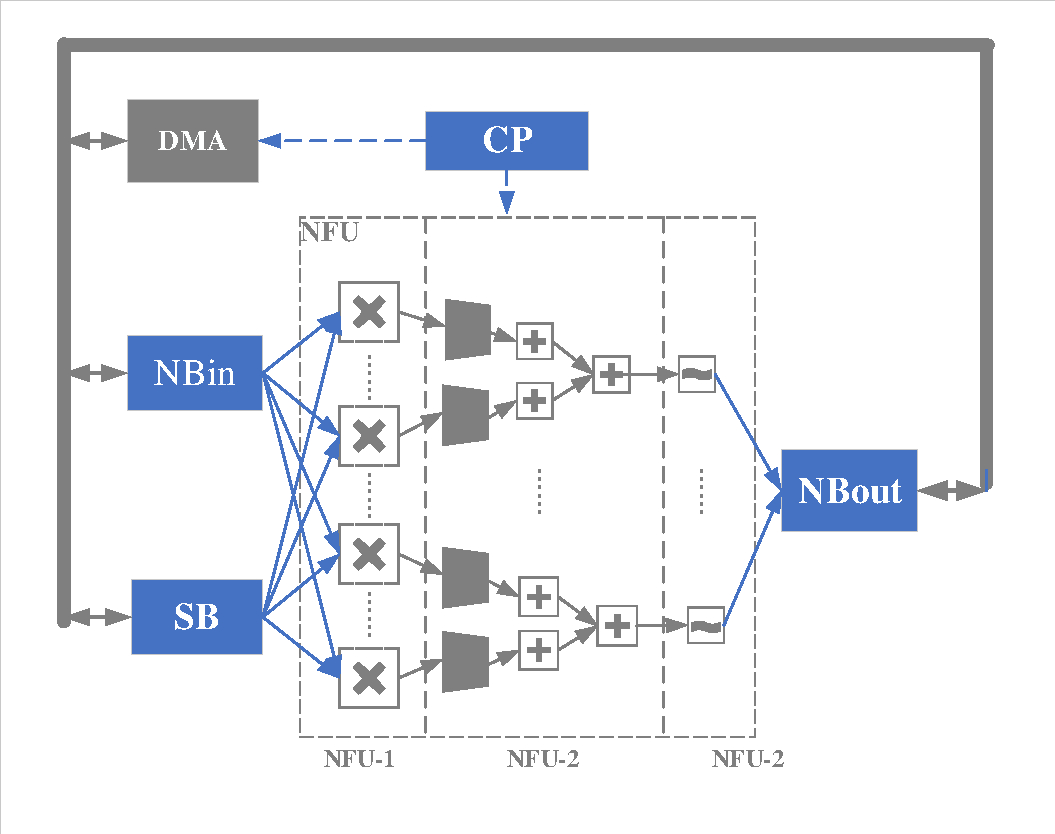
\includegraphics[width=1.0\columnwidth]{diannao.pdf}
  \caption{\footnotesize (a)DianNao加速器结构。(b)DaDianNao一个tile的结构。 (c)DaDianNao一个node的结构}
  \label{fig:diannao}
\end{figure}

\subsection{基于向量算子的神经网络处理器}
DianNao是世界上首个深度神经网络处理器,它的结构如图~\ref{fig:diannao}所示。DianNao包含以下的主要模块:一个控制器(Control Processor,简称CP),一个神经功能单元(Neural Functional Unit, 简称NFU),三个片上缓存(NBin,NBout和SB)和外部存储接口(Memory Interface)。CP采用自定义的指令控制DianNao的运行。NBin,NBout和SB分别用来缓存输入神经元,输出神经元和权值。NFU包含$T_n$个计算单元,每个计算单元包含$T_n$个乘法器和一个$T_n$输入的加法树。在计算过程中每个计算单元共享输入神经元,接收不同的权值,从而计算不同的输出神经元。因此NFU最多读取$T_n$个输入神经元,$T_nxT_n$个权值,计算$T_n$个输出神经元。在TSMC65nm工艺下,采用$T_n$=16的配置,DianNao的面积,功耗和吞吐率分别为$3.02mm^2$,$485mW$和$452GOP/s$,对比与一个2GHz的CPU,能够获得117倍的性能提升,并且降低21倍的能耗。

DadianNao是DianNao的多核版本,一个NFU与外围的存储模块构成一个tile,多个tile通过fat-tree进行局部互联组成一个node,最终多个node通过HyperTransport2.0互联形成DaDianNao。DaDianNao使用eDRAM来提供足够的片上缓存用来存储权值和神经元,从而减少片外访存开销,进而有效地处理大规模神经网络。实验显示,在ST28nm的工艺下,64核的DaDianNao的面积和功耗分别是$67.73mm^2$和$15.97W$,对比Nvidia K20,平均性能提升21.38倍,平均能耗降低了330.56倍。

PuDianNao是一个机器学习处理器,它不仅支持神经网络算法,而且支持K最近邻算法(K-Nearest Neighbors,简称K-NN),K均值算法(K-Means),线性回归(Liner Regression,简称LR),支持向量机(Support Vector Machine,简称SVM),朴素贝叶斯(Naive Bayes,简称NB)和决策树(Classification Tree,简称CT)等多种机器学习算法。PuDianNao深入分析上述机器学习算法,并且提取出机器学习中的核心运算,其中包括向量内积(LR、SVM和DNN),距离计算(K-NN和K-Means),计数(CT和NB),排序(K-NN和K-Means),非线性函数(如sigmoid和tanh)等。PuDianNao的核心模块是机器学习单元(Machine Learning Unit,简称MLU),如图x所示,MLU包括六个流水级,分别为Counter,Adder,Multiplier,Adder Tree,Acc和Misc,通过这六个流水级的组合,PuDianNao能够完成机器学习的核心运算。实验显示,在65nm的共一下,PuDianNao的面积和功耗分别为$3.51mm^2$和$596mW$分为对比NVIDIA K20能够提高1.2倍的性能并且减少129.41倍的能耗。

然而随着神经网络算法的飞速发展,一些新的层类型和新的操作不断涌现,如ROI Pooling层,Deconvolution层等,这又迫使研究者开发新的加速器和指令集来支持这些新的层和操作。为了进一步提高神经网络加速器的通用性,Liu等人提出了针对神经网络处理器的指令集Cambricon。Cambricon的主要思想是为神经网络加速器提供一系列的基本算子(即指令),然后通过这些基本算子逐步搭建完成神经网络的运算。Cambricon中集成了控制,数据传输,运算和逻辑操作这四种不同的指令,其中运算指令进一步分为矩阵运算,向量运算和标量运算指令,研究者只需要基本指令就能完成神经网络的运算。基于Cambricon指令集设计的加速器能够比DaDianNao拥有更强的通用性,在10个benchmark中,DaDianNao只能支持其中的三种,而基于Cambricon的加速器能够全部支持。同时对比与Intel Xeon E5-2620和NVIDIA K40,加速器能够分别获得91.72倍和3.09倍的性能提升。

\subsection{基于乘加算子空间数据流的神经网络处理器}
ShiDianNao是面向嵌入式设备的神经网络处理器,实现端到端的神经网络应用。ShiDianNao的架构如图x所示,ShiDianNao与DianNao最大的不同是NFU模块。ShiDianNao的NFU是一个大小为$P_x\times P_y$的二维处理单元阵列(Processing Elements, 简称PEs),它采用脉动阵列的形式完成神经网络矩阵向量运算操作。每个PE在每个周期能够完成卷积层、全连接层的一次乘法和一次加法,或者平均池化层的一次加法或者最大池化层的比较操作。每个PE能够从右方邻居和下方邻居读取神经元,并且能将部分和传播给相邻的PE,值得注意的是权值通过广播的形式传送给PE。这种方法能够充分复用神经元和权值,从而提高性能并降低访存能耗。在$P_x=P_y=8$的配置下使用65nm工艺,ShiDianNao的主频,面积和功耗分别为$1GHz$,$4.86mm^2$和$320.1mW$,对比GPU和DianNao能够分别获得30倍和1.87倍的加速比,减少4700倍和60倍的能耗。除了ShiDianNao,Farabet等人提出的Neuflow,Chen等人提出的Eyeriss和谷歌的TPU(tensor processing unit)均采用二维网格的形式排列处理单元,并且采用脉动阵列的形式完成神经网络运算。其中Google的TPU主要用来加速其第二代人工智能系统TensorFolow的运行,并且相比于K80能够有15倍的性能提升。


\subsection{稀疏神经网络处理器}
虽然上述加速器能够以低能耗实现高吞吐量,但它们不能利用现代压缩神经网络的稀疏性和不规则性。最近出现了一些能够支持稀疏的神经网络加速器~\cite{chen2017eyeriss,zhang2016cambricon,albericio2016cnvlutin,han2016eie,han2017ese,angshuman2017scnn}
,但它们都有各自的优缺点,如表~\ref{tab:comp}所示。

Eyeriss~\cite{chen2017eyeriss}应用游程压缩方法(run-length-compression,RLC)对稀疏神经元进行编码,具体来说,它在架构中加入RLC Encoder对输出神经元进行压缩,同时采用RLC Decoder对输入神经元进行解压缩,从而减少访问DRAM的数据量,进而减少DRAM的带宽需求和访存能耗。同时Eyeriss在PE单元中加入控制门,当输入神经元为0时,PE单元将被关闭,这样能够跳过不必要的计算,从而减少计算能耗。然而,这两种方法仅仅能够带来能耗的减少,不会带来性能增益。

Cambricon-X~\cite{zhang2016cambricon}能够充分挖掘稀疏权值带来的收益,包括减少能耗和提升性能。Cambricon-X使用步长索引的形式压缩静态的权值,从而减少片外和片上访存能耗开销。同时Cambricon-X利用索引模块(indexing module,IM)来挖掘稀疏的特性,IM能够通过稀疏的权值位置信息过滤掉不需要参与计算的神经元。IM模块的结构如图x所示,首先,IM模块连续地累加权值索引表的值(也就是图中的 1132),这些累加后的值就是每个连接相对起始点的位置,然后采用MUX的逻辑就能选出与非零权值对应的神经元(即n1,n2,n5,n7)。Cambricon-X对比不支持稀疏特性的DianNao提高了7.23倍的性能,并减少了6.43倍的能耗,但是Cambricon-X并不能挖掘稀疏神经元带来的收益。

Cnvlutin~\cite{albericio2016cnvlutin}能够利用动态神经元稀疏筛选出需要进行计算的权值,从而获得1.37倍的加速比,但是Cnvlutin不能利用权值稀疏特性。ESE~\cite{han2017ese}是实现在FPGA上的加速器,它面向的是稀疏的LSTM模型,并不适用于稀疏的CNN模型;由于LSTM模型中使用Tanh作为激活函数,因此不存在神经元稀疏的特性,所以ESE仅仅能够挖掘权值稀疏的特性。

以上工作只能挖掘权值稀疏性或者神经元稀疏性,但不能同时从两者中受益。EIE~\cite{han2016eie}采用稀疏矩阵的行压缩形式(compressed sparse row,简称CSR)存储稀疏的权值,并且通过LZND(leading non-zero detection)筛选出非零的神经元,使得使得EIE能够同时利用神经元稀疏性和权值稀疏性,对比与DaDianNao能够提高2.9倍的性能,减少19倍的能耗并且缩小3倍的面积。但是这种架构仅仅针对全连接层的计算,并不能针对卷积层进行计算。

SCNN~\cite{angshuman2017scnn}能够同时利用神经元稀疏性和权值稀疏性。SCNN中的计算单元构成了一个二维网格的形式,每个计算单元执行非零神经元和非零权值的乘法操作,同时计算非零乘积的坐标。非零乘积通过坐标在二维计算网络进行路由,最终被分配给对应的累加器阵列,每个非零乘积通过读取修改写入操作对包含部分和的本地RAM执行累加,最终获得输出神经元。但是这种架构需要不断计算坐标,大大增加了计算成本和存储成本。因此SCNN在处理稠密神经网络时的会损失$21\%$的性能,同时增加$33\%$的能耗;在处理稀疏神经网络时仅仅能够增加2.7倍的性能,减少2.3倍的能耗。同时SCNN对全连接层和规模为1x1的卷积层支持并不理想,在这两种类型的层时时只能利用$20\%$的乘法器资源。
 

\chapter{一种新的神经网络压缩方法}

\section{背景}
现代神经网络由多种类型的层组成,输入在这些层中不断被传递和处理,从而被分类或识别。在每一层中,每一个神经元接收多个输入进行处理,并将输出通过突触送到下一层。目前主流的神经网络包括卷积神经网络神经网络 (CNNs) ,深度神经网络 (DNNs) 和循环神经网络(RNNs)。目前深层神经网络已经在图像识别, 目标检测,语音识别,自然语言处理,视频处理领域有了越来越广泛的应用。虽然这些神经网络非常强大,但是大规模的神经网络参数(包括神经元和权值)对存储和带宽提出了很高的需求,例如,AlexNet的网络规模超过$200MB$,VGG-16的网络规模超过$500MB$,这使得这些大规模的深度神经网络难以在嵌入式设备,特别是移动设备上进行部署。

首先,对于百度和Facebook等公司,手机端的各种应用程序更新都是通过不同的应用程序商店进行下载,它们是对二进制文件的大小非常敏感。例如,应用程序商店会限制当应用程序大于$200MB$时,必须连接无线网络才能够进行下载。因此,当应用超过$200MB$时,将会收到比$10MB$应用更多的安全审查。尽管在手机端本地运行深度神经网络能够减少网络带宽,进行任务实时处理,获得更好的隐私保护,但是这些大规模的神经网网络需要耗费巨大的存储开销,因此阻碍了深度神经网络被纳入移动应用程序。

第二个问题是能耗消耗。运行大型神经网络需要大量的带宽和计算资源来获得神经网络数据,并进行计算,这个过程需要耗费巨大的能耗。考虑到移动设备电池容量的限制,高能耗的应用,如深层神经网络将难以部署。能源消耗主要是内存访问。在45纳米工艺下,一个32位浮点加法需要消耗$0.9pJ$的能量,一次32位SRAM缓存访问耗费$5pJ$的能量,而一次32位DRAM内存访问需要$640pJ$的能量,这个能耗几乎是浮点加法操作的3个数量级。大型神经网络无法缓存在片上的SRAM中,因此需要能耗更高的DRAM访问。例如我们以$20fps$运行一个拥有10亿个连接的神经网络,那么需要为DRAM访存提供至少$P = (20Hz)\times (640pJ)\times (1G) = 12.8W$的功率,这个已经完全超过了大多数手机电池能够提供的功率。

\subsection{神经网络中的稀疏特性}
虽然现代神经网络在许多应用中占主导地位,但是庞大的参数给计算、内存容量和内存访问带来了沉重的负担。为了应对这些挑战,研究者从各个方向做出了各种各样的努力,包括算法级 (例如Drop out~\cite{srivastava2014dropout}、Sparsity~\cite{han2015learning}),架构级 (例如短位宽运算~\cite{holi1993finite}甚至是1比特运算~\cite{rastegari2016xnor}、非精确计算~\cite{venkataramani2014axnn})和物理级(例如,动态电压调整技术~\cite{pillai2001real})。其中,稀疏技术是目前解决这个问题最有效的方法。研究人员在早期工作中已经证明了稀疏性是解决过拟合问题的有效方法。对于现代神经网络,研究者们提出了一系列的训练技术,如稀疏编码 (Sparse Encoder)~\cite{olshausen1996emergence},自动编解器 (Auto Encoder/Decoder)~\cite{boureau2008sparse,lee2008sparse}, 深度信念网络 (Deep Belief Network, DBN)~\cite{lee2007efficient}等,在步影响精度的前提下修剪冗余的突触和神经元。最近,研究人员提出了一种新的剪枝方法,在CNNs上获得了非常理想的稀疏性,在AlexNet~\cite{krizhevsky2012imagenet}网络上获得了$88.85\%$的稀疏度, 在VGG16~\cite{simonyan2014very}网络上获得了$92.39\%$的稀疏度。在表~\ref{tab:deepratio},我们报告详细的剪枝结果,这里,我们定义稀疏度 (sparsity) 为被修剪的神经元/突触占总神经元/突触的比例,同时我们定义稠密度(density)为非零神经元/突触占总神经元/突触的比例。


\begin{figure}[h]
  \centering
  \begin{minipage}[t]{\columnwidth}
  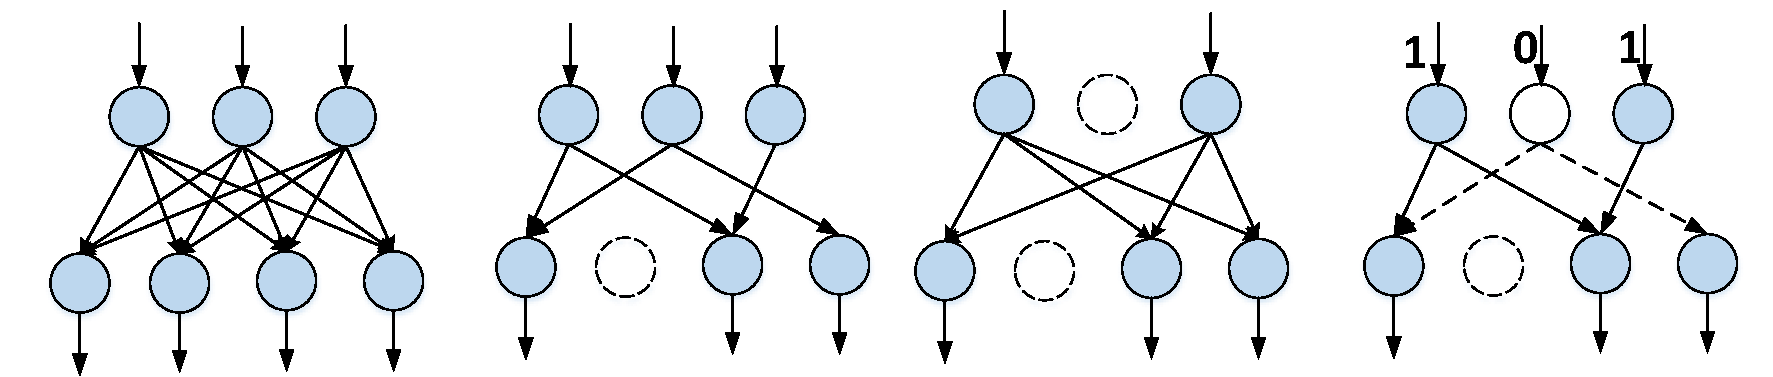
\includegraphics[width=1.0\columnwidth]{sparse_network.pdf}
  \end{minipage}
  \vfill
  \begin{minipage}[t]{0.24\columnwidth}
      \centering\footnotesize
    (a)
  \end{minipage}
  \hfill
  \begin{minipage}[t]{0.24\columnwidth}
      \centering\footnotesize
    (b)
  \end{minipage}
  \hfill
  \begin{minipage}[t]{0.24\columnwidth}
      \centering\footnotesize
    (c)
  \end{minipage}
    \hfill
  \begin{minipage}[t]{0.24\columnwidth}
      \centering\footnotesize
    (d)
  \end{minipage}
  \caption{ (a) 稠密神经网络 (b) 静态权值稀疏 (c) 静态神经元稀疏 (d) 动态神经元稀疏}
  \label{fig:sparsity}
\end{figure}

如图~\ref{fig:sparsity}所示,我们将神经网络中的稀疏分为两类:\emph{静态稀疏 (static sparsity)}和\emph{动态稀疏 (dynamic sparsity)}。\emph{静态稀疏}源于剪枝操作,当突触 (图~\ref{fig:sparsity} (b)) 或者神经元 (图~\ref{fig:sparsity} (c)) 满足某些条件时,它们将从神经网络的拓扑结构中被永久剪除,因此这种稀疏又被称为\emph{静态稀疏}。当神经元的输出值为$0$时(图~\ref{fig:sparsity} (d))会发生\emph{动态稀疏}, 特别是当使用ReLU作为激活函数时,在ReLU激活之前结果为负的神经元输出值为$0$。形式上,ReLU用如下公式计算输出神经元
\begin{equation}
ReLU(x)=
\begin{cases}
x & \text{if } x > 0, \\
0 & \text{if } x \leq 0
\end{cases}
\end{equation}
其中$x$为ReLU激活函数的输入,$yR$为ReLU的输出。因此,像ReLU这样的激活函数可以在网络的神经中中引入许多$0$。不同于~\emph{静态稀疏},\emph{动态稀疏}不改变网络拓扑结构,它与输入密切相关,因为不同的输入将导致不同的计算结果,从而导致不同的动态稀疏结果。值得注意的是,\emph{静态稀疏}又可以分为\emph{静态权值稀疏 (static synapse sparsity, SSS)}和~\emph{静态神经元稀疏 (static neuron sparstiy, SNS)},\emph{动态稀疏}仅由\emph{动态神经元稀疏 (dynamic neuron sparsity, DNS)}组成。

\subsection{权值编码}

\begin{figure}[h]
\centering
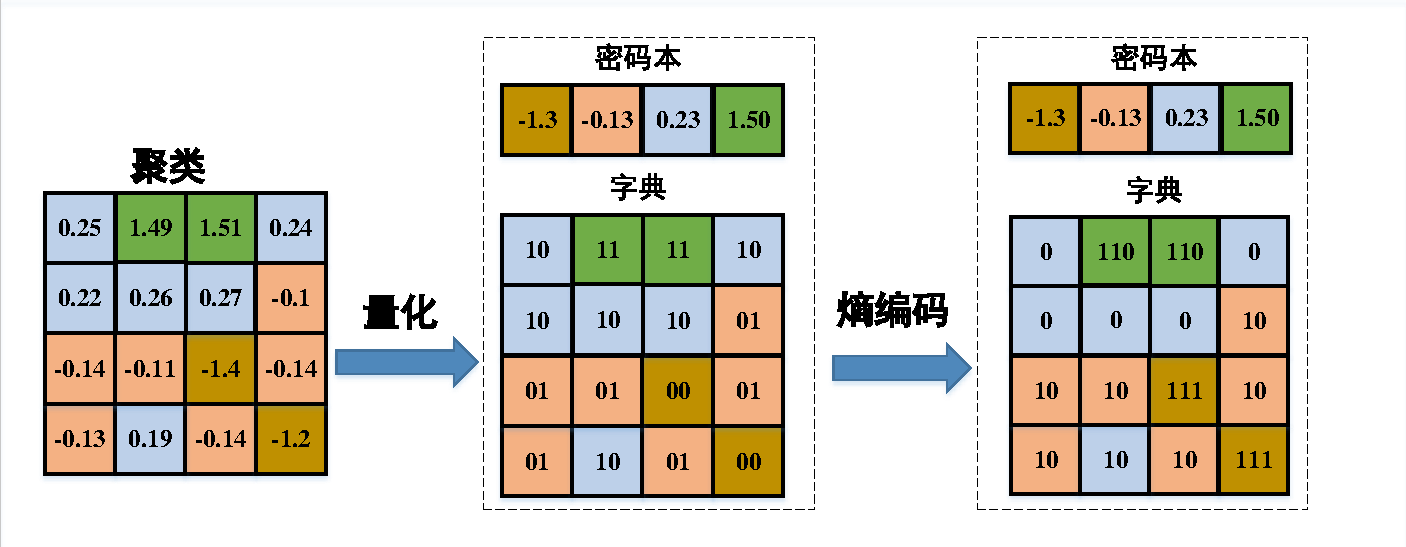
\includegraphics[width=1.0\columnwidth]{WE.pdf}
\caption{权值编码过程}
\label{fig:weight_encoding}
\end{figure}

为了进一步压缩权值数据,研究人员将图像压缩技术,如量化 (quantization)~\cite{henneaux1992quantization},熵编码 (entropy coding)~\cite{mackay2003information}等应用到神经网络的领域。Deep Compression~\cite{han2015deep}运用细粒度剪枝,全局量化和霍夫曼编码对神经网络进行深度压缩,在基本不损失精度的情况下,在AlexNet网络上获得35倍的压缩比。另一种有效的压缩方案是CNNpack~\cite{wang2016cnnpack},它在频域中对神经网络进行深度压缩,最终在AlexNet网络上获得了40倍的压缩比。我们在图~\ref{fig:weight_encoding}中描述了权值编码的过程,它由量化和熵编码两个步骤组成。

\subsubsection{量化}
首先,我们利用聚类算法 (例如,K-means聚类) 将分散的权重聚集成$K$簇。在图中,16个权值被分为4个簇,其中 (0.25, 0.24, 0.22, 0.26, 0.27, 0.19)这六个权值被聚为一个簇。然后我们计算每个簇的中心值,该值与簇中所有权重的总距离最小,每一个权值都用它所在簇的质心值来近似表示,例如在图中,(0.25, 0.24, 0.22, 0.26, 0.27, 0.19)这六个权值都用0.23表示。因此,我们可以用一个密码本和一个字典来表示所有权值,其中密码本中记录了$K$个簇中的中心值,字典中每个元素只需要$log(K)$位来索引密码本从而获得权值。

\subsubsection{哈弗曼编码}

\begin{figure}[h]
\centering
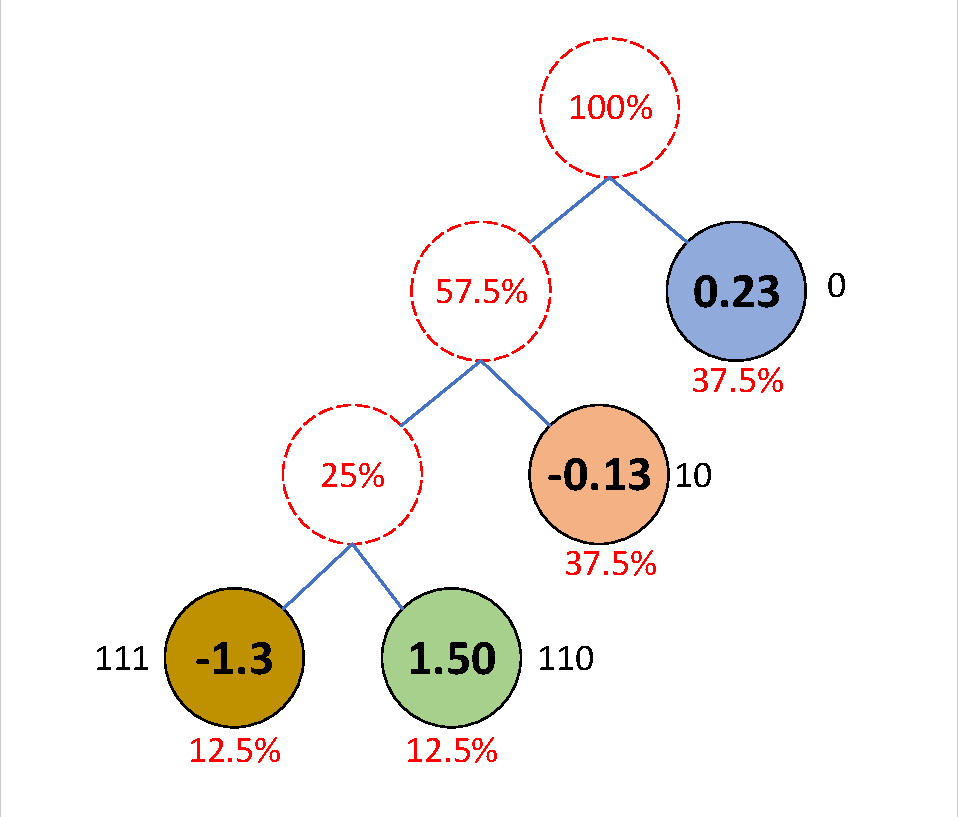
\includegraphics[width=0.6\columnwidth]{huffman.pdf}
\caption{哈弗曼树}
\label{fig:huffman}
\end{figure}

由于密码本中元素的出现概率是不平衡的,因此我们可以采用熵编码(如哈弗曼编码)进一步降低权重的比特数。哈弗曼编码方法完全依赖于码字出现的概率来构造整体平均长度最短的编码方法。进行哈夫曼编码的关键步骤是建立符合哈夫曼编码规则的二叉树,该树又称作哈夫曼树。哈夫曼树是一种特殊的二叉树,其终端节点的个数与待编码的码元的个数等同,而且每个终端节点上都带有各自的权值。每个终端节点的路径长度乘以该节点的权值的总和称为整个二叉树的加权路径长度。在满足条件的各种二叉树中,该路径长度最短的二叉树即为哈夫曼树。在使用哈夫曼编码执行对码元的实际编码过程时,通过递归地合并概率最小的码元来构建哈夫曼树。以图~\ref{fig:weight_encoding}为例,四个码元-1.3,-0.13,0.23,1.50出现的概率分别是0.125,0.375,0.375,0.125,最终可以构造出如图~\ref{fig:huffman}所示的哈弗曼树。在哈夫曼树构建完成后,便可以得到每一个码元的哈夫曼编码的码字。具体方法是:从哈夫曼树的根节点开始遍历,直至每一个终端节点,当访问某个节点的左子树时赋予码字1,访问右子树时赋予一个码字0(反之亦然),直到遍历到终端节点时这一路径所代表的0和1的串便是该码元的哈夫曼编码码字。最终四个码元-1.3, -0.13, 0.23, 1.50分别被编码成为是111,10,0,110。

\subsection{不规则性}
尽管稀疏神经网络能够在理论上减少计算量,存储量和数据传输量,但是稀疏会导致原本规则的神经网络计算模式转变为不规则的形式。然而,目前的处理平台由于存在诸多问题,无法有效地处理稀疏性。根据~\cite{zhang2016cambricon},CPU和GPU并不能很好地支持稀疏神经网络运算,即使使用稀疏矩阵运算库,如sparseBLAS或者cuBLAS,也不能取得非常理想的加速效果,在某些情况下处理稀疏网络的性能甚至比处理稠密神经网络的性能还要差。尽管目前又不少支持稀疏神经网络的加速器~\cite{zhang2016cambricon, albericio2016cnvlutin, han2016eie, han2017ese, angshuman2017scnn},但是它们仍然不能有效地处理稀疏神经网络带来的不规则性。他们需要显著的稀疏成本,而且不能完全支持所有稀疏类型,例如Cambricon-X~\cite{zhang2016cambricon}中支持稀疏的逻辑占总面积的$31.07\%$,占功耗的$34.83\%$,而且只能支持权值稀疏。因此,我们需要一种新的神经网络稀疏方法,能够在保持高的精度和稀疏度条件下尽可能保持神经网络的规则性,减少稀疏神经网络的不规则性,有利于CPU,GPU或者加速器能够充分利用稀疏带来的收益。


\section{局部收敛 (local convergence)}

\begin{figure}[h]
  \centering
  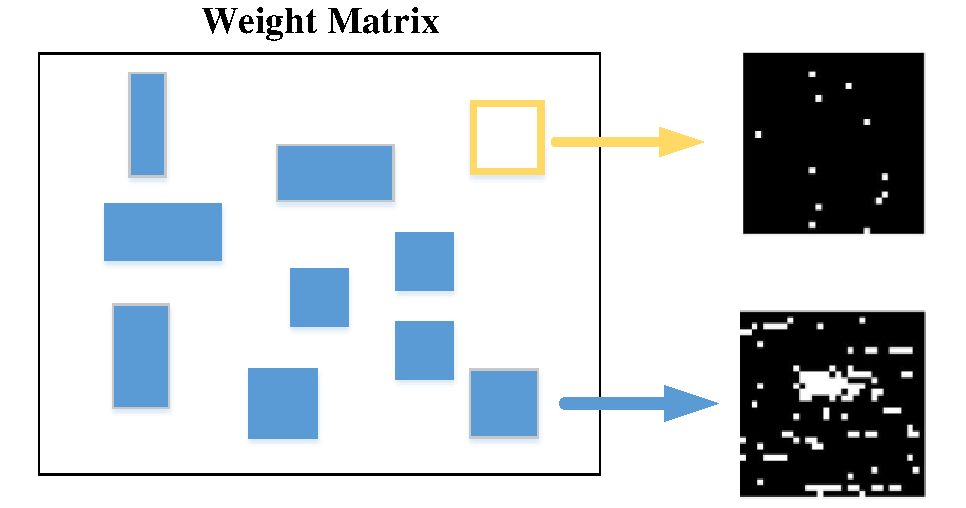
\includegraphics[width=0.8\columnwidth]{local_convergence.pdf}
  \caption{全连接层中的局部收敛现象(白点表示大权值,绝对值大于其余$90\%$的权值)}
  \label{fig:local_convergence}
\end{figure}

传统的剪枝方法将每一个突触当作独立不相关的元素,当突触符合特定的剪枝条件时(如权值的绝对值小于某一个阈值),该突触将会被剪除,但是这种方式忽略了突触之间的潜在关系。我们充分分析了神经网络中的权重分布情况,观察到了一个有趣的现象。如图~\ref{fig:local_convergence}所示,我们使用权值矩阵来表示全连接层的权值,每一行包含与对应输入神经元相连接的所有权值,每一列包含与对应输出神经元相连接的所有权值;我们可以发现,绝对值大的权值往往会聚集成簇,我们将这种现象称为局部收敛(local convergence)。我们利用如下的方式证明局部收敛的存在。首先,我们在权值矩阵上设定一个大小为$k$的滑动窗口,然后将该滑动窗口沿着权值矩阵空间维度上进行滑动(全连接层权值矩阵为两个维度,卷积层权值矩阵为四个维度),同时统计窗口中较大权值的数量,如果某一个权值的绝对值大于剩余$m\%$的权值,我们将其定义为较大的权值。为了方便阐述,我们将一个具有$x$个大权值的窗口标记为$x$窗口。我们选择了5个代表性的层: AlexNet网络的~\emph{fc6}层, VGG16网络的~\emph{fc6}层, MLP网络的~\emph{ip1}层, LSTM网络的~\emph{$W_{ix}$}层, AlexNet网络的~\emph{conv2}作为驱动示例。我们将前四层网络的滑动窗口大小设为$k = 4$, \emph{conv2}层网络的滑动窗口大小设为$k = 2$,此外,我们将$m = 90$设置为较大权值的阈值。在图~\ref{fig:cdf}中,我们描绘了一个随机初始化层与训练后的5个层中较大权值的累计分布。我们观察到,在初始化层中,同一个窗口中较大权值的数量不会超过四个。但是,这五个训练过的层存在同一个窗口中较大权值的数量超过七个的情况。因此,较大权值在训练过程中趋向于聚集在一起,也就是局部收敛。

\begin{figure}[t]
\centering
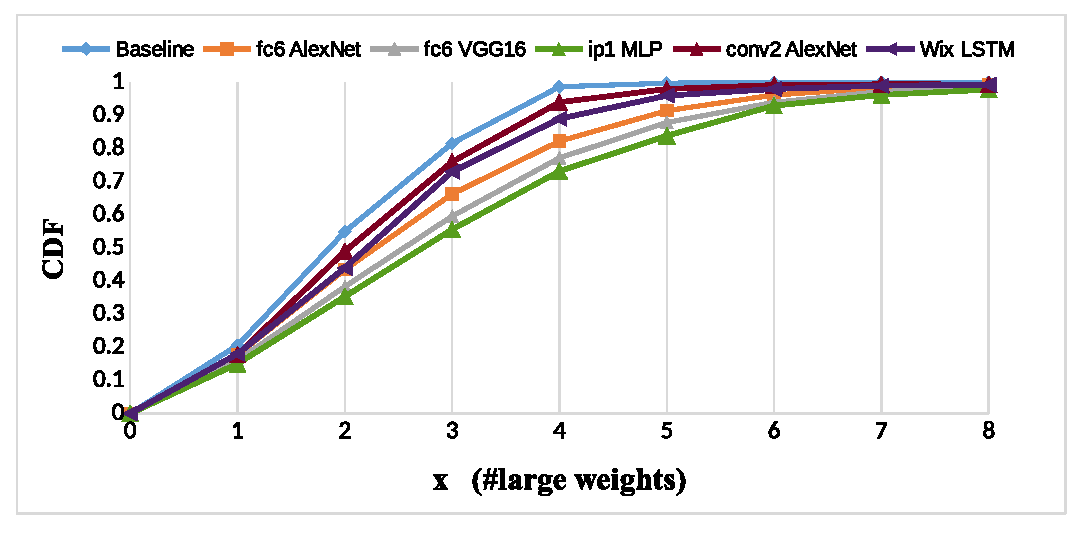
\includegraphics[width=0.8\columnwidth]{CDF.eps}
\caption{较大权值的累计分布}
\label{fig:cdf}
\end{figure}

\section{压缩神经网络}

\begin{figure}[h]
\centering
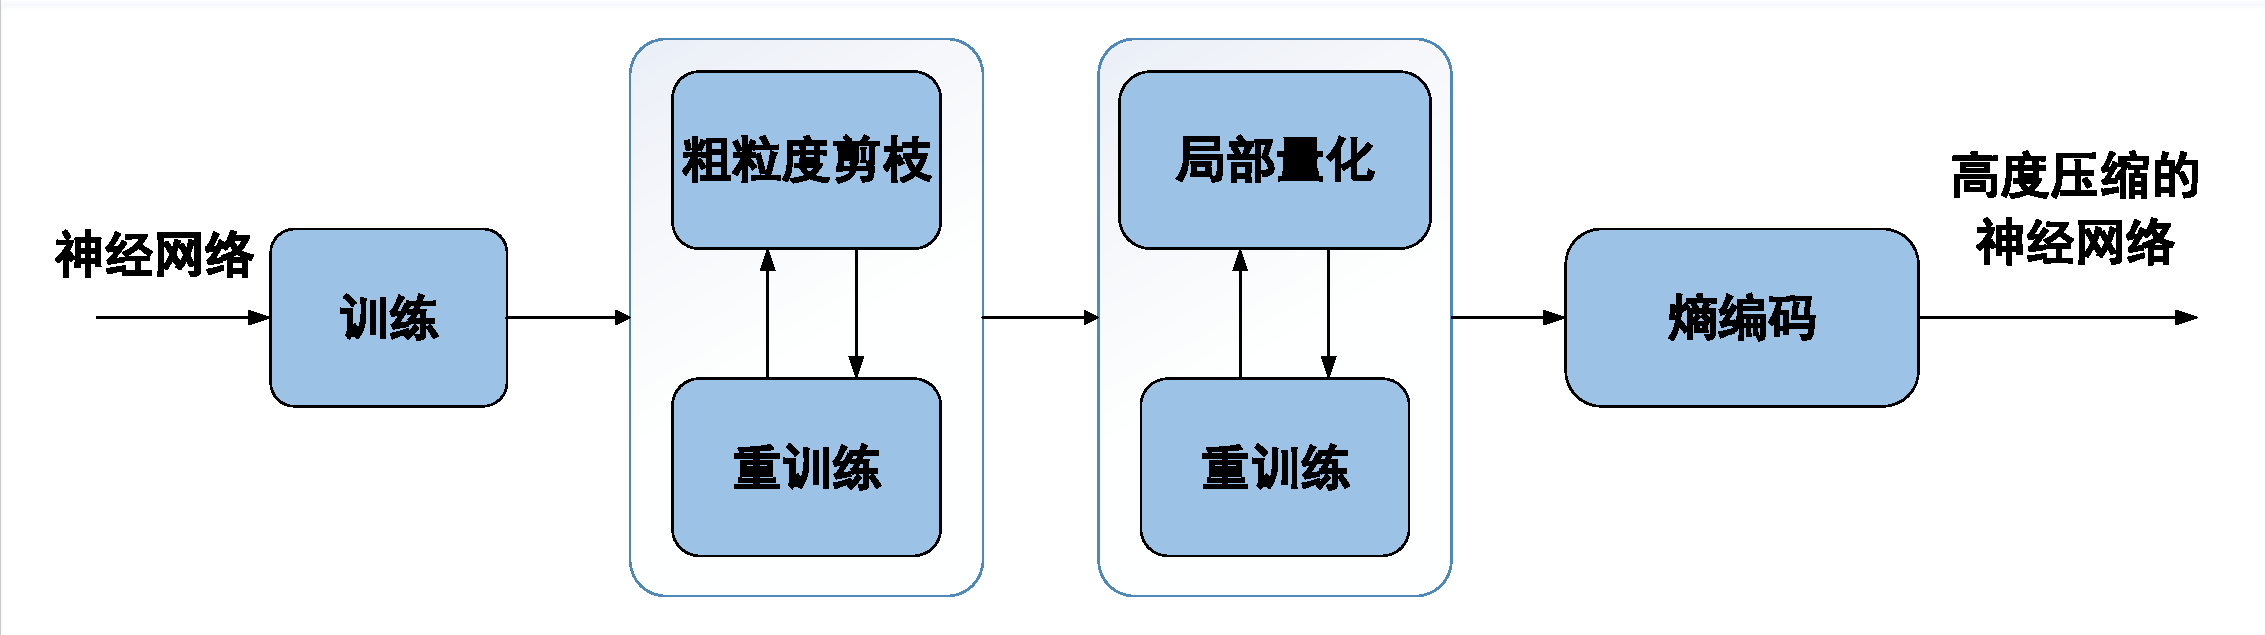
\includegraphics[width=1.0\columnwidth]{compression_flow.pdf}
\caption{新的压缩神经网络步骤}
\label{fig:compression_flow}
\end{figure}

如图~\ref{fig:compression_flow}所示,我们提出了一种新的压缩神经网络的方法,整个流程包括三个步骤:粗粒度剪枝,局部量化和熵编码。下面我们将依次详细阐述这三个步骤。


\subsection{粗粒度剪枝}

我们提出了一种新的剪枝策略:粗粒度剪枝。粗粒度剪枝的核心思想基于神经网络局部收敛的特征,我们将多个突触同时进行剪枝操作,而不是对单个权值进行剪枝。我们首先将权值矩阵分成多个块,如果某一个符合特定的条件,这个权值块将在网络拓扑中被永久剪除,然后我们使用较小的学习率对网络进行重训练,从而保持网络的准确性。值得注意的是,我们在训练中迭代地应用粗粒度剪枝和重训练,以获得更好的稀疏性,同时避免精度损失。为了清晰地解释粗粒度剪枝技术,我们使用全连接层~\ref{fig:fc_pruning}和卷积层~\ref{fig:conv_pruning}作为驱动示例。

\subsubsection{剪枝策略}

\begin{figure}[h]
\centering
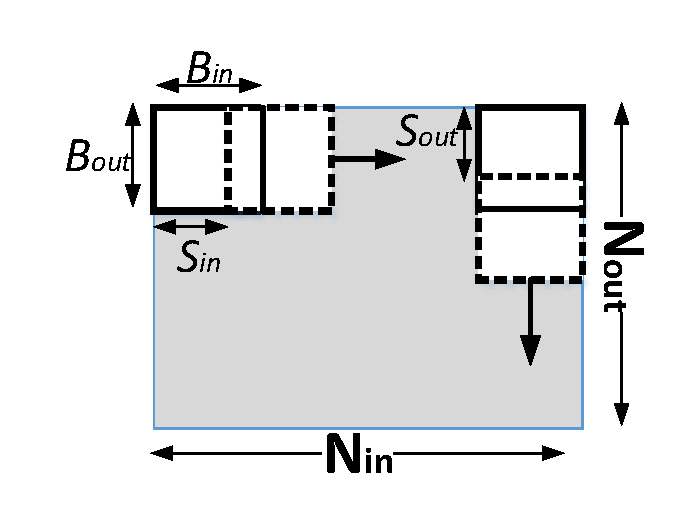
\includegraphics[width=0.7\columnwidth]{fc_pruning.pdf}
\caption{全连接层上的粗粒度剪枝}
\label{fig:fc_pruning}
\end{figure}

在一个全连接层中,($N_{out}$)个输出神经元通过二维权值矩阵($N_{out}$, $N_{in}$)与($N_{in}$)个输入神经元,如图6所示。在剪枝过程中,大小为$B_{in} \times B_{out}$的滑动窗口沿着权值矩阵的两个维度分别按照$S_{in}$和$_{out}$的步长进行滑动。一旦滑动窗口中的权值某些条件,窗口内的突触都会同时被剪枝。在迭代剪枝过程中,滑动窗口将跳过修剪过的突触,使所有修剪过的突触块都具有相同的规模大小,从而简化索引过程。

对于卷积层,输出特征图中的输出神经元通过共享的突触连接到输入特征图中的神经元。因此,卷积层中的权值可以表示为一个四维张量,即$(N_{fin},N_{fout},K_x,K_y)$,其中$N {fin}$是输入特征图的数量,$N {fout}$是输出特征图的数量,和$K x$,$K_y$是卷积核的大小。如图所示,在剪枝过程中,大小为$B_{fin} \times B_{fout} \times B_x \times B_y$的滑动窗口沿着四维的权值张量分别按照$S_{fin}$,$S_{fout}$,$S_x$和$S_y$的步长进行滑动。

\begin{figure}[h]
  \centering
  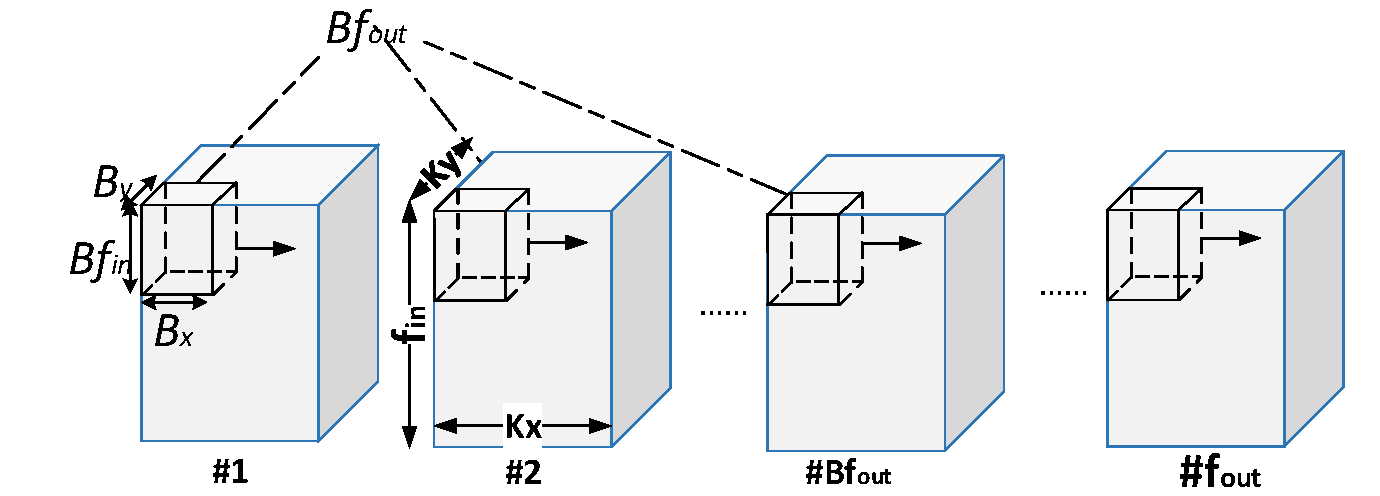
\includegraphics[width=1.0\columnwidth]{conv_pruning.pdf}
  \caption{卷积层上的粗粒度剪枝}
  \label{fig:conv_pruning}
\end{figure}

\subsubsection{剪枝块大小}

在粗粒度剪枝过程中,寻找最佳的剪枝块大小来权衡压缩比与精度之间的平衡至关重要。使用过大的块进行剪枝将导致突出连接无法完全表达神经网络的特性,从而降低准确性。使用过小的块进行剪枝,并不能充分利用局部权值收敛的特性,从而无法获得很高的压缩比。值得注意的是,如果我们将剪枝块的大小设定为1,那么粗粒度的剪枝就是~\cite{han2015learning}中的细粒度剪枝。

在本文中,我们仔细权衡神经网络中不同类型层的块大小来修剪不同的网络。理论上,我们应该为不同的层选择剪枝块大小,而不是为不同类型的层选择剪枝块大小,但是考虑到在庞大的设计空间搜索和极长训练时间,我们关注的是为网络中不同类型的层设定剪枝块大小。例如,由于卷积层中的权值比全连接层的权值更敏感,因此我们只在卷积层的某个维度上进行粗粒度剪枝。我们以AlexNet为作为驱动实例,在保持网络准确性的同时,阐述不同剪枝块的大小对神经网络稀疏度和压缩效果的影响。如表~\ref{tab:blocksize}所示,我们将AlexNet网络的基准精度设定为top-1误差$42.8\%$,同时我们使用$(1,N,1,1)$和$(N,N)$的剪枝块分别对卷积层和全连接层进行粗粒度剪枝。在表2中,我们将卷积层和全连接层的权值分别用8位和4位进行量化,然后用Huffman编码进行编码。当$N$从1增加到64时,压缩比$r_c$首先从40倍迅速增长到79倍,然后迅速下降到65倍。当剪枝块从1增大到16时,压缩比随之增加,主要原因是非零权值索引所需的存储空间不断减少。当剪枝块大小从16增加到64时,压缩比随之下降,这是因为为了保持相同的精度,神经网络的稀疏度不断降低(卷积层稀疏度从$64.75\%$降低到$54.45\%$),从而阻碍了压缩比。为了更好地平衡压缩比和精度,我们将卷积层中的剪枝块大小设置为$(1,16,1,1)$,将fc6,fc7和fc8的剪枝块大小分别设定为$(32,32)$,$(32,32)$和$(16,16)$。值得注意的是,使用粗粒度剪枝,非零权值索引所需要的存储空间只需要$29.38KB$,相比于使用细粒度剪枝后~\cite{han2015deep}的索引($2.95MB$)减少了102.82倍。

\begin{table}[b]
\centering
\caption{ 不同剪枝块大小情况下AlexNet网络的稀疏度和压缩比(C: 卷积层;F: 全连接层; S: 稀疏度; $r_c$ 压缩比)}
\label{tab:blocksize}
\begin{tabular}{lll@{~}llll@{~}llll@{~}llll@{~~}llll@{~~}llll@{~~}llll@{~~}lllllllll}
\toprule
N  				& 1 	&  2		& 4			& 8			& 16		& 32 		&64		\\
\midrule
C:S(\%)			& 64.99 &64.99		&64.89		&64.77		&64.75		&59.95		&54.45 	\\
F:S(\%) 		& 89.99	&89.98		&89.98		&89.97		&89.95		&89.91		&87.78	\\
Weight (MB)     & 2.86 	&2.86		&2.87		&2.87		&2.91		&3.01		&3.59	\\
Index (MB)      & 2.95	&0.76		&0.22		&0.07		&0.03		&0.01		&0.005	\\
$r_c$ 			& $40\times$ 	&$64\times$		&$75\times$		&$79\times$		&$79\times$		&$77\times$		&$65\times$	\\
\bottomrule
\end{tabular}
\end{table}

\subsubsection{最大值剪枝 vs. 平均值剪枝}

\begin{figure}[t]
  \centering
  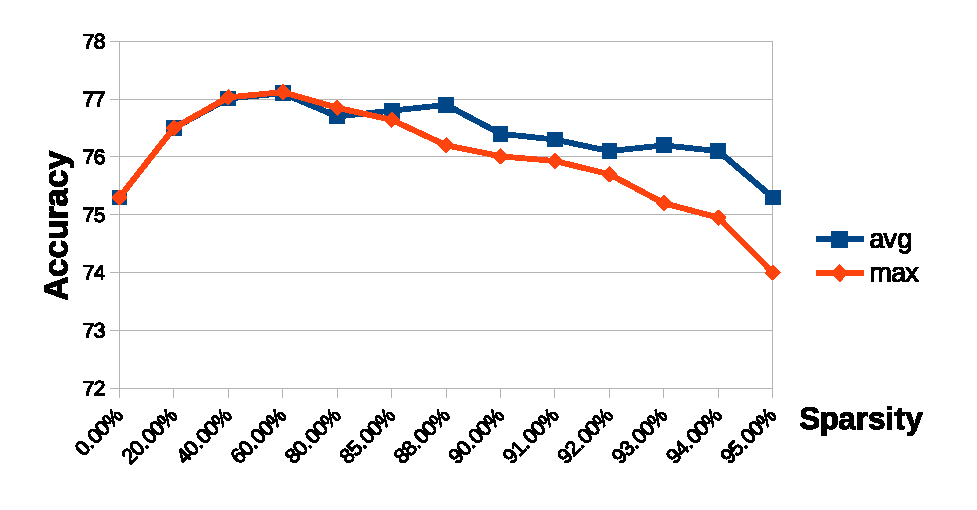
\includegraphics[width=1.0\columnwidth]{avg_max.eps}
  \caption{Cifar10快速模型上的最大值剪枝和平均值剪枝}
  \label{fig:max_or_avg_pruning}
\end{figure}

在粗粒度剪枝过程中,我们可以使用两种不同的剪枝策略,第一种是最大值剪枝策略,第二种是平均值剪枝策略。对于最大值剪枝策略,如果窗口中具有最大绝对值的权值小于预定义阈值($W_{th}$),则将窗口中的所有权值剪除。对于平均值剪枝,如果窗口中所有权值绝对值的平均值小于预定义的阈值,则将窗口中的所有权值剪除。这两种剪枝策略的主要特性是完全不同的。最大值剪枝表明只有块内部最大的权重才会影响整个块的重要性。平均值剪枝表明,块内的所有权重将对块的重要性产生影响。我们使用这两种剪枝方法在Cifar10快速模型上进行粗粒度剪枝和训练,在剪枝过程中我们控制这两种剪枝方法使用相同大小的滑动窗口和步长。图~\ref{fig:max_or_avg_pruning}显示,当神经网络的稀疏度高于$85\%$时,平均值剪枝比最大值剪枝精度更高。因此,本文选择了平均值剪枝的策略。

\subsubsection{不规则性的评估方法}
为了更直观地表现粗粒度剪枝的效果,我们提出了一种简单而有效的方法来定量测量粗粒度剪枝减少的不规则性。我们使用如下公式计算
\begin{equation}
R(Irr) = JBIG(I_f)/JBIG(I_c)
\end{equation}
其中$R(Irr)$表示减少的不规则性,$I_{f}$和$I {c}$分别表示经过细粒度剪枝和粗粒度剪枝后稀疏神经网络的索引,$JBIG()$表示基于Joint Bi-level Image ExpertsGroup~\cite{jbig}的无损二值图像压缩标准。这种方法基于这样一个事实:常规数据(特别是二进制矩阵)包含了更多的冗余信息,因此可以用更少的数据来表示。因此,我们将突触索引作为二进制图像,用JBIG压缩它们。压缩后的数据大小在某种程度上可以衡量数据的不规则性。因此,我们通过粗粒度剪枝与细粒度剪枝后压缩索引大小之比来度量降低的不规则性。

\subsubsection{神经元稀疏}
在粗粒度的剪枝过程中,我们只修剪突触,并不会对神经元进行直接修剪,仅仅当某个神经元与其他神经元之间没有任何连接时,该神经元会被剪除,因此静态神经元稀疏的比例并不高。然而,在大型网络中,动态神经元稀疏占了很大的比例,即神经元经过激励后的输出值为0的情况。在表x中显示了在各个网络中,权值稀疏性,静态神经元稀疏性和动态神经元稀疏性。在大规模神经网络中,如AlexNet、VGG16和ResNet-152,静态神经元稀疏性非常低,在卷积层中接近$0\%$,即基本不会出现静态神经元的情况。然而,在AlexNet和VGG16中,动态神经元稀疏性却很有前景,在AlexNet中为$37.63\%$,在VGG16为$59.48\%$,动态神经元稀疏为提高计算性能和节省能耗提供了很好的契机。

\begin{table}[b]
\centering
\caption{\footnotesize 神经网络中的稀疏性 (C: 卷积层; F:全连接层; SSS: 静态权值稀疏; SNS: 静态神经元稀疏; DNS: 动态神经元稀疏).}
\label{tab:sparsities}
\begin{tabular}{@{~}lll@{~}lll@{~}lll@{~}lll@{~}lll@{~}lll@{~}llllllllllll}
\toprule
-- & LeNet5 & MLP & Cifar10 & AlexNet & VGG16 & ResNet152 \\
%\hline
\midrule
C: SSS (\%)& 88.98 	& -- 	& 92.08 & 64.75 & 64.83 & 45.69 \\
   SNS (\%)& 25.39	& -- 	& 11.49 & 0.00 	& 0.00 	& 0.00 \\
   DNS (\%)& 0.00	& -- 	& 30.61 & 37.63	& 59.48 & 50.30 \\
\hline
F: SSS (\%)& 91.47	& 90.13	& 93.99 & 89.95	& 95.16 & 0 \\
   SNS (\%)& 47.70	& 40.25 & 57.73 & 15.75 & 22.18	& 0 \\
   DNS (\%)& 11.50	& 66.31 & 19.93	& 29.27 & 43.03	& 24.10 \\
\bottomrule
\end{tabular}
\end{table}

\subsection{局部量化}
\begin{figure}[h]
  \centering
  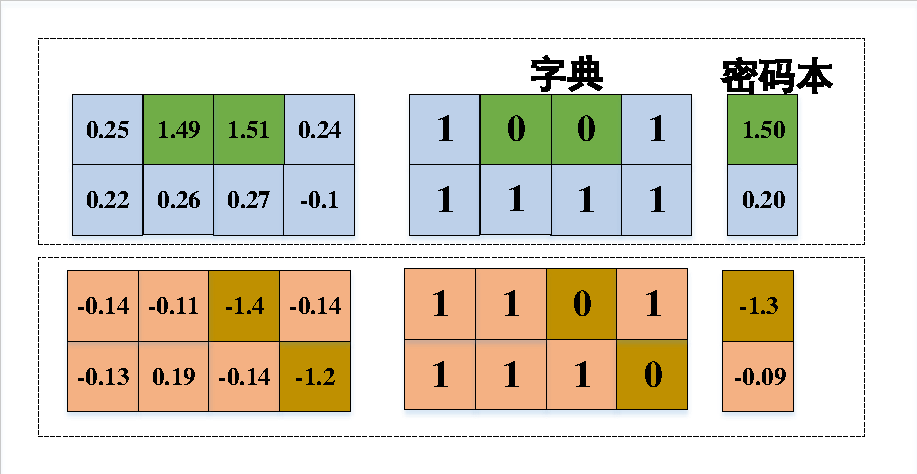
\includegraphics[width=1.0\columnwidth]{LQ.pdf}
  \caption{局部量化}
  \label{fig:local_quantization}
\end{figure}
应用权值共享和网络量化的策略可以有效地减少代表权值的比特位~\cite{han2015deep}。为了更好地利用局部收敛的特性,我们提出了局部量化的策略,不同于全局量化在整个权值矩阵中进行权值共享,局部量化仅仅在权值矩阵的局部区域中进行权值共享。如图~\ref{fig:local_quantization}所示,局部量化策略首先将权值矩阵划分为两个子矩阵,然后对两个子矩阵分别进行聚类。在每个子矩阵中,权值将被编码成一个密码本和一个字典,其中字典中的每个权值只需要1比特进行索引(使用图~\ref{fig:weight_encoding}中的全局量子化方法,密码本中每个权值需要2比特进行索引)。与全局量化相比,局部量化能够利用局部收敛来进一步减少表示权值的比特数,从而获得更高的压缩比。值得注意的是局部量化的开销很小,以AlexNet网络的fc6层为例,全局量化需要一个$128B$的密码本和$2.0MB$的字典,其中字典中每个元素需要5比特进行索引;局部量化过程中我们将权值矩阵分为64个小矩阵,因此需要64个密码本和64个对应的字典,但是字典中每个元素仅仅需要4比特进行索引,因此密码本和字典的大小分别为$4KB$和$1.6MB$,对比与全局量化存储容量减小了$19.81\%$。

\subsection{熵编码}
熵编码是一种无损的数据压缩策略,它为输入中的每个符号创建并分配唯一的无前缀码。由于每个码字的长度都与该符号出现概率的负对数成比例,所以我们使用更少的比特来编码出现概率更高的符号。目前两种最常见的熵编码技术是Huffman coding~\cite{huffman1952method}和算术编码~\cite{witten1987arithmetic}。实验显示,熵编码能够进一步减少$20\% - 30\%$的网络存储开销。

\subsection{压缩实验结果}
\begin{table}[h]
\centering
\caption{压缩后神经网络的稀疏度,压缩比和不规则性减少量 ($W_p$: 粗粒度剪枝后权值规模 ; $W_q$: 粗粒度剪枝,局部量化后权值规模; $W_c$: 粗粒度剪枝,局部量化,熵编码后权值规模; L: \emph{LSTM}层 ; C: 卷积层; F: 全连接层; W: 权值; I:权值索引;$r_p$: 粗粒度剪枝后压缩比; $r_q$: 粗粒度剪枝,局部量化后压缩比; $r_c$: 粗粒度剪枝,局部量化,熵编码后压缩比; $R(Irr)$: 不规则性减少量)。}
\label{tab:compression}
\begin{tabular}{@{}l@{~}l@{\!\!}l@{~}l@{\,}l@{~}l@{\,}l@{}l@{~}l@{~}l@{~}l@{~}lll}
\toprule
Model		&\!\!\!Sparsity(\%) & ~~$W_p(B)$ 	& $r_p$ 	& $W_q(B)$ 		& $r_q$ 		& $W_c(B)$ 		& $r_c$			& $R(Irr)$ 				\\
\midrule
Alexnet 	& C: 64.75\ 		&W: 25.65M  &$9\times$   &W: 3.60M 		& $64\times$ 	& W: 2.90M		& $79\times$	& $101.65\times$	 				\\
  			& F: 89.93\ 		&I: 36.73K  &  			 &I: 36.73K 	&  	 			& I: 29.38K 	& 				&		\\
%\hline
VGG16 		& C: 64.83\ 		&W: 42.72M  &$12\times$  &W: 7.80M		& $66\times$ 	& W: 5.25M 		& $98\times$	& $28.54\times$  	 				\\
  			& F: 95.16\  		&I: 202.80K &			 &I: 202.80K 	&  	  			& I: 121.68K	& 	  	 		&			\\
%\hline
LeNet-5 		& C: 88.98\ 		&W: 135.96K &$12\times$  &W: 23.77K 	& $66\times$  	& W: 19.01K		& $82\times$	& $8.87\times$ 	 				\\
  			& F: 91.47\  		&I: 1.67K   &			 &I: 1.67K		&  	   			& I: 1.39K 						& \\
%\hline
MLP 		& C: --				&W: 102.54K &$10\times$  &W: 19.23K 	& $51\times$  	& W: 12.01K 	& $82\times$ 	& $10.41\times$				\\
  			& F: 90.13\  		&I: 1.20K   &			 &I: 1.20K		&  				& I: 0.61K	 	&  				& 		\\
%\hline
Cifar10 	& C: 92.08\			&W: 42.08K  &$13\times$	 &W: 8.68K 		& $62\times$   	& W: 7.82K		& $69\times$ 	& $7.61\times$			\\
  			& F: 93.99\  		&I: 0.48K   &			 &I: 0.48K		&  		       	& I: 0.42K  	&				& \\
%\hline
ResNet152 	& C: 45.69\			&W: 134.10M &$1.7\times$ &W: 33.50M		& $7\times$  	& W: 23.44M		& $10\times$ 	& $13.02\times$					\\
  		    & F: 0.00\ 		    &I: 0.49M   &			 &I: 0.49M		&				&  I: 0.44M		&	 			& \\

%\hline
LSTM 		& L: 87.94  		&W: 1.50M 	&$8.3\times$  &W: 191.28K 	& $60\times$	& W: 152.47K 	& $77\times$	& $50.51\times$							\\
  			&   				&I: 25.96K   & 			 &I: 25.96K 		&			& I: 17.84K	  	& 				&		\\
\bottomrule
\end{tabular}
\end{table}

在表~\ref{tab:compression}中,我们列出了七个神经网络的详细压缩结果,这七个神经网络包括LeNet-5~\cite{lecun1998gradient}, MLP~\cite{Srivastava2014} (三层神经网络,包含$300\times 100$个隐层神经元),Cifar10快速模型~\cite{krizhevsky2012cuda},AlexNet~\cite{krizhevsky2012imagenet},VGG16~\cite{simonyan2014very},ResNet152~\cite{he2016deep}和LSTM~\cite{sak2014long}。注意,我们只关注LSTM模型中的LSTM层。
我们在表中详细地罗列了各个神经网络能够获得的稀疏度(Sparsity),经过三个压缩步骤(即粗粒度剪枝,局部量化,熵编码)后神经网络的规模(分别用$W_p$,$W_q$和$W_c$表示)和压缩比(分别用$r_p$,$r_q$和$r_c$表示),同时我们还罗列了粗粒度剪枝减少的不规则性($R(Irr)$)。我们的压缩算法在AlexNet, VGG16, LeNet-5, MLP, Cifar10, ResNet152和LSTM网络上分别获得了79倍,98倍,82倍,92倍,69倍,10倍和77倍的压缩比,造成了精度损失小于$0.2\%$,平均减少不规则度20.13倍。

在表~\ref{tab:deepratio}中,我们将压缩方法与现有的两种最先进的神经网络压缩方法进行了比较,即Deep Compression~\cite{han2015deep} (细粒度剪枝) 和CNNpack~\cite{wang2016cnnpack}(频域压缩)。我们的压缩方法获得的压缩比几乎是Deep Compression和CNNpack的两倍,获得这么高压缩比的主要原因是我们的压缩算法能够显著减少神经网络的不规则度,从而显著减少权值索引信息的存储空间。值得注意的是,我们的压缩算法除了能够获得高压缩比,还能获得与Depp Compression类似的稀疏度,同时精度损失几乎可以忽略不计。对于ResNet网络,我们的压缩方法和Deep Compression只能获得不到10倍的压缩比,远远低于传统的神经网络。出现这种现象的原因是ResNet网络中包含多种新的特性,包括快捷连接(shortcut connections)和批处理归一化(batch normalization),这些特性从而大大缓和了神经网络的过拟合的现象。因此,我们在ResNet中只能获得一个非常有限的压缩比。

与表~\ref{tab:deepratio},我们将我们压缩算法的准精确与Deep Compression和CNNpack进行比较。我们可以看出,我们的压缩方法造成的精度损失是可以忽略不计的。与参考准确度相比,我们的压缩方法的精度损失低于$0.2\%$,类似于Deep Compression($0.1\%$),并且低于CNNpack($0.7\%$)。

表~\ref{tab:compression}还列出了粗粒度剪枝减少的不规则性。值得注意的是,粗粒度的剪枝可以将不规则性平均减少20.13倍,剪枝的块越大,不规则性减少的程度就越高。对于小型网络,如LeNet-5、MLP和Cifar10,减少的不规则性平均是8.80倍,因为我们只能用比较小的剪枝块对小的神经网络进行修剪,减少精度损失。相反,大型网络,如AlexNet、VGG16和LSTM,减少的不规则性要大得多,平均是52.71倍,因为我们可以选用更大的剪枝快对神经网络进行修剪。另外,对于ResNet网络,考虑到新特性,我们只能用比较小的剪枝块来修剪它,能够减少13.02倍的不规则性。实验结果进一步证实粗粒度剪枝可以显著降低网络的不规则性。

\begin{table}[t]
\centering
\caption{\footnotesize CNNPack, Deep Compression 与我们的压缩方法的对比 (S\%: 稀疏度; $r_c$: 压缩比).}
\scriptsize
\label{tab:deepratio}
\centering
\begin{tabular}{l@{~~}@{~~}lll@{~~}lll@{~~}lllll@{~~}lll@{~~}lll@{~~}lllll@{~~}lll@{~~}lll@{~~}ll}
\toprule
model 	& Ref 				& \multicolumn{3}{c}{Deep Cmp.~\cite{han2015deep}} 	& \multicolumn{3}{c}{CNNpack~\cite{wang2016cnnpack}} 	& \multicolumn{3}{c}{Ours}				\\
  		& Top1-E(\%) 		& S (\%) & $r_c$ & Top1-E(\%) 	 					& S (\%) & $r_c$ & Top1-E(\%)  	 						&S (\%) & $r_c$ & Top1-E(\%) 		\\
\midrule
AlexNet  	& 42.78			& 88.85	& $35\times$ 	& 42.78 							& --	 &  $39\times$  & 41.60 (41.80$^{\star}$) 				 		& 88.97 & $79\times$	& 42.72				\\
VGG16		& 31.50			& 92.39	& $49\times$ 	& 31.17								& --	 &  $46\times$  & 29.70 (28.50$^{\star}$)							& 91.93  & $98\times$ 	& 31.33				\\
LeNet-5 	& 0.80			& 91.57	& $39\times$ 	& 0.74 								& --	 &  --   & --									& 91.40  & $82\times$ 	& 0.95			 	\\
MLP 		& 1.64			& 91.82	& $40\times$ 	& 1.58								& --  	 &  -- 	 & -- 									& 90.13  & $82\times$ 	& 1.91				\\
Cifar10 	& 24.20			& 94.98	& $45\times$ 	& 24.33								& --	 &  --   & -- 									& 92.93  & $69\times$   & 24.22				\\
ResNet152 	& 25.00			& 45.00 & $8\times$		& 24.40 							& --	 &  --	 & -- 									& 44.17 & $10\times$ 	& 25.05				\\
LSTM 		& 20.23			& 88.47 & $35\times$ 	& 20.52								& --	 &  --   & --									& 87.94	& $77\times$ 	& 20.72				\\
\bottomrule
\end{tabular}
%\\\raggedright\scriptsize{$^{\star}$Reference accuracies used in~\cite{wang2016cnnpack}.}
\end{table}

\begin{table}[h]
\centering
\caption{AlexNet压缩特征 (W: 权值; S\%: 稀疏度 I: 权值索引).}
\begin{tabular}{llllll}
\toprule
layer  	& \#W 	& S\%		& bits per W	& W size(KB)& I size(KB) \\
\midrule
conv1 	& 35K	& 24.9		& 6.5 			& 20.75 	& 0.80 \\
conv2 	& 307K	& 65.5		& 5.6 			& 72.45 	& 3.23 \\
conv3 	& 885K	& 64.1		& 5.4 			& 209.37 	& 9.69 \\
conv4 	& 663K	& 66.6		& 6.2 			& 167.73 	& 6.76 \\
conv5 	& 442K 	& 65.9		& 5.5 			& 101.28 	& 4.61 \\
\midrule
fc6 	& 38M 	& 91.1	& 3.3			& 1353.37	& 1.60 \\
fc7 	& 17M 	& 91.10		& 3.4 			& 626.69 	& 0.72 \\
fc8 	& 4M 	& 74.8		& 3.3 			& 415.80	& 1.97 \\
\midrule
total	& 61M	& 88.9		& 3.7			& 2967.44	& 29.38 \\
\bottomrule
\label{tab:AlexNet}
\end{tabular}
\end{table}

此外,我们在表~\ref{tab:AlexNet}列出了AlexNet网络的详细压缩特性。卷积层和fc6,fc7,fc8层的块大小分别为$(1, 16, 1, 1,)$,$(32, 32)$,$(32, 32)$,$(16,16)$。我们将卷积层和全连接层的权值分别量化为8比特和4比特。表中的权值和权值索引采用了都用Huffman编码。值得注意的是,与权值大小相比,权值索引大小几乎可以忽略不计。而在Deep Compression中,权值索引信息几乎是总存储容量的40\%,这严重阻碍了更有效的压缩。此外,使用细粒度的修剪时,权值和权值索引分别是$25.93MB$和$3.24MB$;使用粗粒度剪枝时,权值大小和索引大小分别是$25.65MB$和$36.73KB$(比细粒度剪枝减少90.32倍)。局部量化进一步将权值大小减小到$3.6MB$,而全局只能将权值大小压缩到$4.95MB$。经过熵编码后,索引大小只有$29.38KB$,对比与Deep Compression的2.95MB缩小102.82倍。受益于粗粒度稀疏和局部量化,我们新的压缩方法可以将AlexNet压缩79倍,远远高于Deep Compression (35倍) 和CNNPack (39倍)。






\chapter{稀疏神经网络加速器的架构}

我们的压缩方法能够对神经网络进行深度压缩,其中粗粒度稀疏能够充分利用神经网络局部收敛的特征,寻找最能够代表神经网络特征的权值块,从而有效减少稀疏权值的不规则性(平均减少20.13倍);局部量化进一步
利用局部收敛的特性,减少表示每个权值的比特数;最后熵编码对神经网络进行进一步的无损压缩。深度压缩的神经网络能够减少数据存储需求,减少计算量,减少数据传输量,最终提高计算性能,减少计算能耗。因此我们设计专用的硬件加速器,为了充分挖掘深度压缩神经网络的优秀特性。新型加速器的最主要的特征是两个选数逻辑:神经元选择模块 (neuron selector module, NSM) 和突触选择模块(synapse selector module, SSM),分别过滤不必要的神经元和权值。同时,我们为加速器设计了专用的基于库的编程模型,减轻用户的编程负担。与最先进的稀疏的神经网络加速器Cambricon-X~\cite{zhang2016cambricon}相比,我们的加速器能够获得1.71倍的加速比,同时减少1.37倍的能耗。在65nm工艺下,我们的加速器面积和功耗仅仅为为$6.73mm^2$和$798.55mW$。

本章中我们首先以一个粗粒度稀疏的全连接神经网络为驱动实例,充分分析神经网络加速器的设计原则。然后我们根据这些设计原则设计对应的神经网络加速器。最后我们为加速器设计了一套基于库的编程框架以减轻用户的编程负担。

\section{设计原则}
\label{sec:principle}

\begin{figure}[ht]
\centering
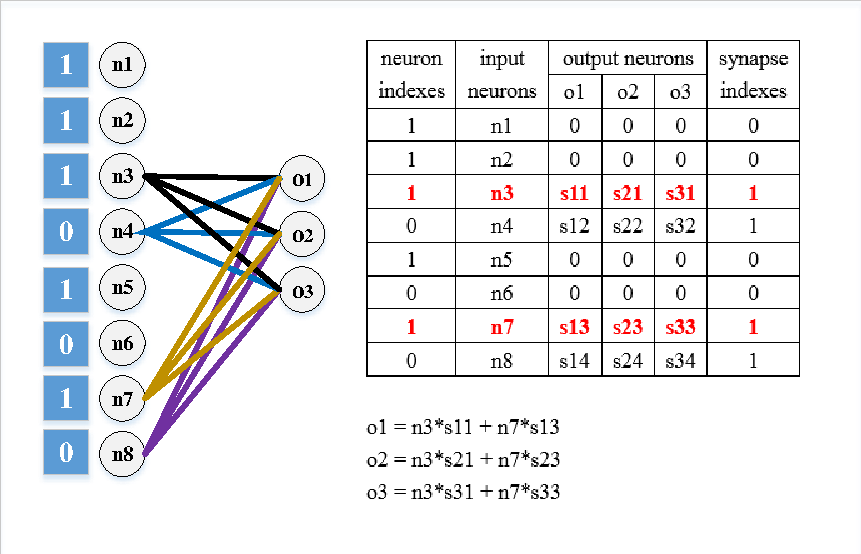
\includegraphics[width=1.0\columnwidth]{connection.pdf}
\caption{粗粒度稀疏的全连接层}
\label{fig:connection}
\end{figure}

我们将使用一个经过粗粒度稀疏的全连接层作为示例(参见图~\ref{fig:connection}),分析粗粒度稀疏神经网络的特性,进而分析出神经网络加速器的设计原则。在图中,我们使用$2\times 3$的剪枝块对全连接层进行剪枝,同时我们只关注其中规模为$8\times 3$的部分连接。由于ReLU激励函数,输入神经元$n4, n6, n8$的激活为“0”。
通过观察,我们发现了以下四个粗粒度稀疏神经网络的特性。

首先,多个输出神经元之间共享索引信息。如图~\ref{fig:connection}所示,输入神经元$n1, n2, n5, n6$与输出神经元$o1, o2, o3$之间的连接被同时剪除,因此输出神经元之间共享相同的连接拓扑,也就是说它们共享相同的权值索引表示~\emph{“00110011”}(图中的“Synapse Indexes”)。尽管输出神经元之间不共享相同的权值,但所选权重的位置是相同的,因此是一种部分共享。

第二,多个输出神经元之间共享输入神经元。如图~\ref{fig:connection}所示,最终需要参与计算的神经元是$n3, n7$,它们的值被输出神经元共享。不失一般性,在完全连接的层中,设定修剪块大小为$(B_{in},B_{out})$,那么$B_{out}$个相邻输出神经元将共享相同的输入神经元。在卷积层中,设定剪枝块的大小为为$(B_{fin},B_{fout},B_x,B_y)$,那么$B_{fout}$个相邻的输出神经元将共享相同的输入神经元。

第三,动态稀疏性能够进一步提高运算效率。在图中,通过挖掘权值稀疏,输入神经元$n3, n4, n7, n8$被筛选出来进行计算,同时由于输入神经元$n4, n8$的激活为零,在运算过程中,它们对输出神经元没有贡献,最后需要进行计算的输入神经元为$n3, n7$。在图中的实例中,通过挖掘权值稀疏性,共需要进行12次乘法,9次加法完成运算;同时挖掘权值稀疏性和动态神经元的稀疏性,只需要进行6次乘法和3次加法。对比在稠密情况下24次乘法和21次加法,分别有2.14倍和5倍的性能提升。因此,利用动态神经元稀疏性是进一步提高效率的关键(在上面的示例中,能够进一步提升2倍性能)。值得注意的是,即使考虑到动态神经元稀疏,输出神经元仍然共享索引和所选的输入神经元。

第四,多个输出神经元之间的负载是平衡的,因为它们共享相同的输入神经元。对于图~\ref{fig:connection}中的示例,如果考虑静态稀疏,那么每个输出神经元共享相同的输入神经元$n3, n4, n7, n8$,同时需要四个对应的权值$S_{Ti1}, S_{Ti2}, S_{Ti3}, S_{Ti4}$进行计算,因此每个输出神经元需要进行4次乘法和3次加法完成运算。如果同时考虑静态稀疏和动态稀疏,那么每次输出神经元共享相同的输入神经元$n3, n7$,同时需要两个对应的权值$S_{Ti1}, S_{Ti3}$进行计算,因此每个输出神经元需要进行2次惩罚和1次加法完成运算。因此粗粒度稀疏的神经网络可以避免负载不平衡而造成的性能损失~\cite{han2017ese}。

因此,在设计加速器时要考虑以下原则,以最大限度地提高加速器的效率:加速器(1)能够利用共享的索引信息和共享的输入神经元信息,简化加速器的设计;(2)能够利用动态稀疏性进一步提高效率;(3)利用相邻输出神经元之间的负载均衡。


\section{加速器架构}
\begin{figure}[h]
\centering
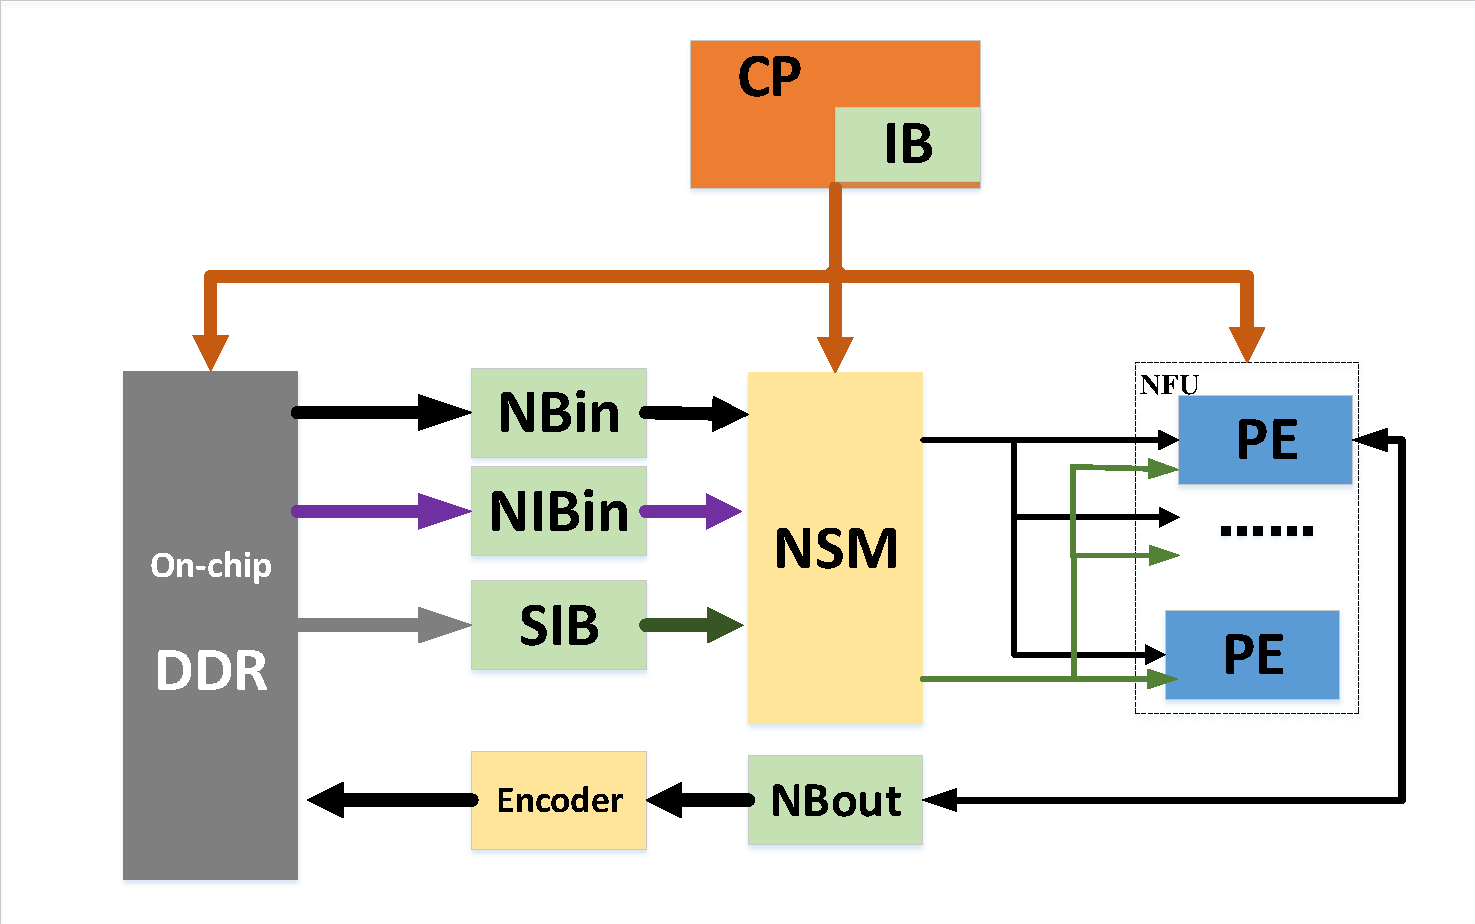
\includegraphics[width=1.0\columnwidth]{ACC.pdf}
\caption{加速器整体架构}
\label{fig:acc}
\end{figure}

在本节中,我们将介绍我们的加速器的详细架构,它能够充分利用深度压缩神经网络带来的收益,有效地解决粗粒度修剪稀疏网络的剩余不规则性。

如图~\ref{fig:acc}所示,我们展示了加速器架构。按照~\ref{sec:principle}的设计原则,我们在加速器中设计了一个关键模块-神经元选择器模块 (neural selector module, NSM),用于处理静态稀疏和共享信息(包括共享索引信息和共享神经元信息)。同时我们设计了一个神经功能单元 (neural functional unit,NFU) 用于完成神经网络中的核心计算。NFU中具有多个处理单元 (processing elements, PEs) 用来并行计算不同的输出神经元。每个PE都包含一个本地的突触选择器模块 (synapse selector module, SSM)来处理动态稀疏性。动态神经元压缩模块 (Encoder)用于动态地将输出神经元压缩成为非零元素/非零元素索引的模式,从而减少Load/Store神经元的开销。存储模块需要存储输入神经元,权值和输出神经元,因此我们需要输入神经元缓存(input neuron buffer, NBin), 输出神经元缓存 (output neuron buffer, NBout) 和突触缓存(synapse buffer, SB),考虑到神经元和权值的稀疏性,我们需要两个额外的缓存,即输入神经元索引缓存(input neuron index buffer, NIBin) 和突触索引缓存(synapse index buffer, SIB) 分别存储输入神经元索引和突出索引信息。注意,其中SB被内置与NFU的每一个PE中,没有表现在图中。控制模块由控制处理器 (control processor, CP) 和指令缓存 (instruction buffer, IB) 组成,CP有效地将IB中存储的各种指令解码为所有其他模块的详细控制信号,这里我们为加速器定义一个VLIW(very long instruction word)风格的指令集。

下面我们将从稀疏处理,存储,控制和片上互联四个方面介绍加速器。

\subsection{稀疏处理单元}
该加速器旨在利用(1)静态稀疏性和(2)动态稀疏性,以及(3)压缩数据,从而减少数据存储量,减少数据传输量,减少计算量,从而提升性能,并减少能耗。在加速器中,稀疏性由NSM,NFU和Encoder这三个模块共同处理。NSM接收来自NBin的输入神经元,来自NIBin的输入神经元索引和来自SIB的权值索引,筛选出需要进行计算的神经元(静态稀疏),同时生成筛选权值的synapse flags,然后将筛选出的神经元和synapse flags通过NFU广播给PE。每个PE中的SSM通过synapse flags筛选出需要进行计算的权值(动态稀疏),从而避免无用的计算和数据传输,提高加速器的性能。最后Encoder动态压缩输出神经元,从而减少片外访存能耗。

\subsubsection{Indexing}
在详细说明NSM,NFU,Encoder之前,我们将详细说明如何在加速器中存储和索引稀疏数据。表示稀疏数据的方法主要有两类,分别是二进制binary mask和numerical indexing,这两类方法都仅存储非零元素,使用不同的方式索引非零元素。Binary mask的方式主要包括直接索引(direct indexing),我们使用比特串对非零元素进行索引,其中"0"表示对应的位置的元素为零,"1"表示对应位置元素为非零。Numerical Indexing 包括步长索引(step indexing),压缩稀疏行(compressed sparse row, CSR),压缩稀疏列(compressed sparse column,CSC),坐标列表查找(coordinate list,COO)等,它们主要使用非零元素之间相对位置(步长)或者绝对位置信息对非零元素进行索引。由于目前主流的神经网络稠密度大小$5\%$,采用CSR,CSC,COO等方式的存储开销远远大于direct indexing或者step indexing的方式;而且考虑到神经元和权值同时稀疏,step indexing这种方式很难索引到两者同时非零的情况,因此我们采用直接索引的方式存储稀疏神经元和稀疏权值。如图~\ref{fig:connection},我们仅需要存储$n1, n2, n3, n5, n7$这五个神经元和~\emph{“11101010”}比特串就能够表示稀疏的输入神经元;同时我们仅需要存储$s11, s12, s13, s14$这四个权值和~\emph{“00110011”}比特串就能够表示与$o1$相连的稀疏突触。值得注意的是,由于稀疏权值是一种静态稀疏,这种压缩过程可以离线完成;但是稀疏神经元是一种动态稀疏,这个过程需要在线实时完成,因此我们需要Encoder模块对稀疏神经元进行动态压缩。

\subsubsection{NSM}
\begin{figure}[h]
\centering
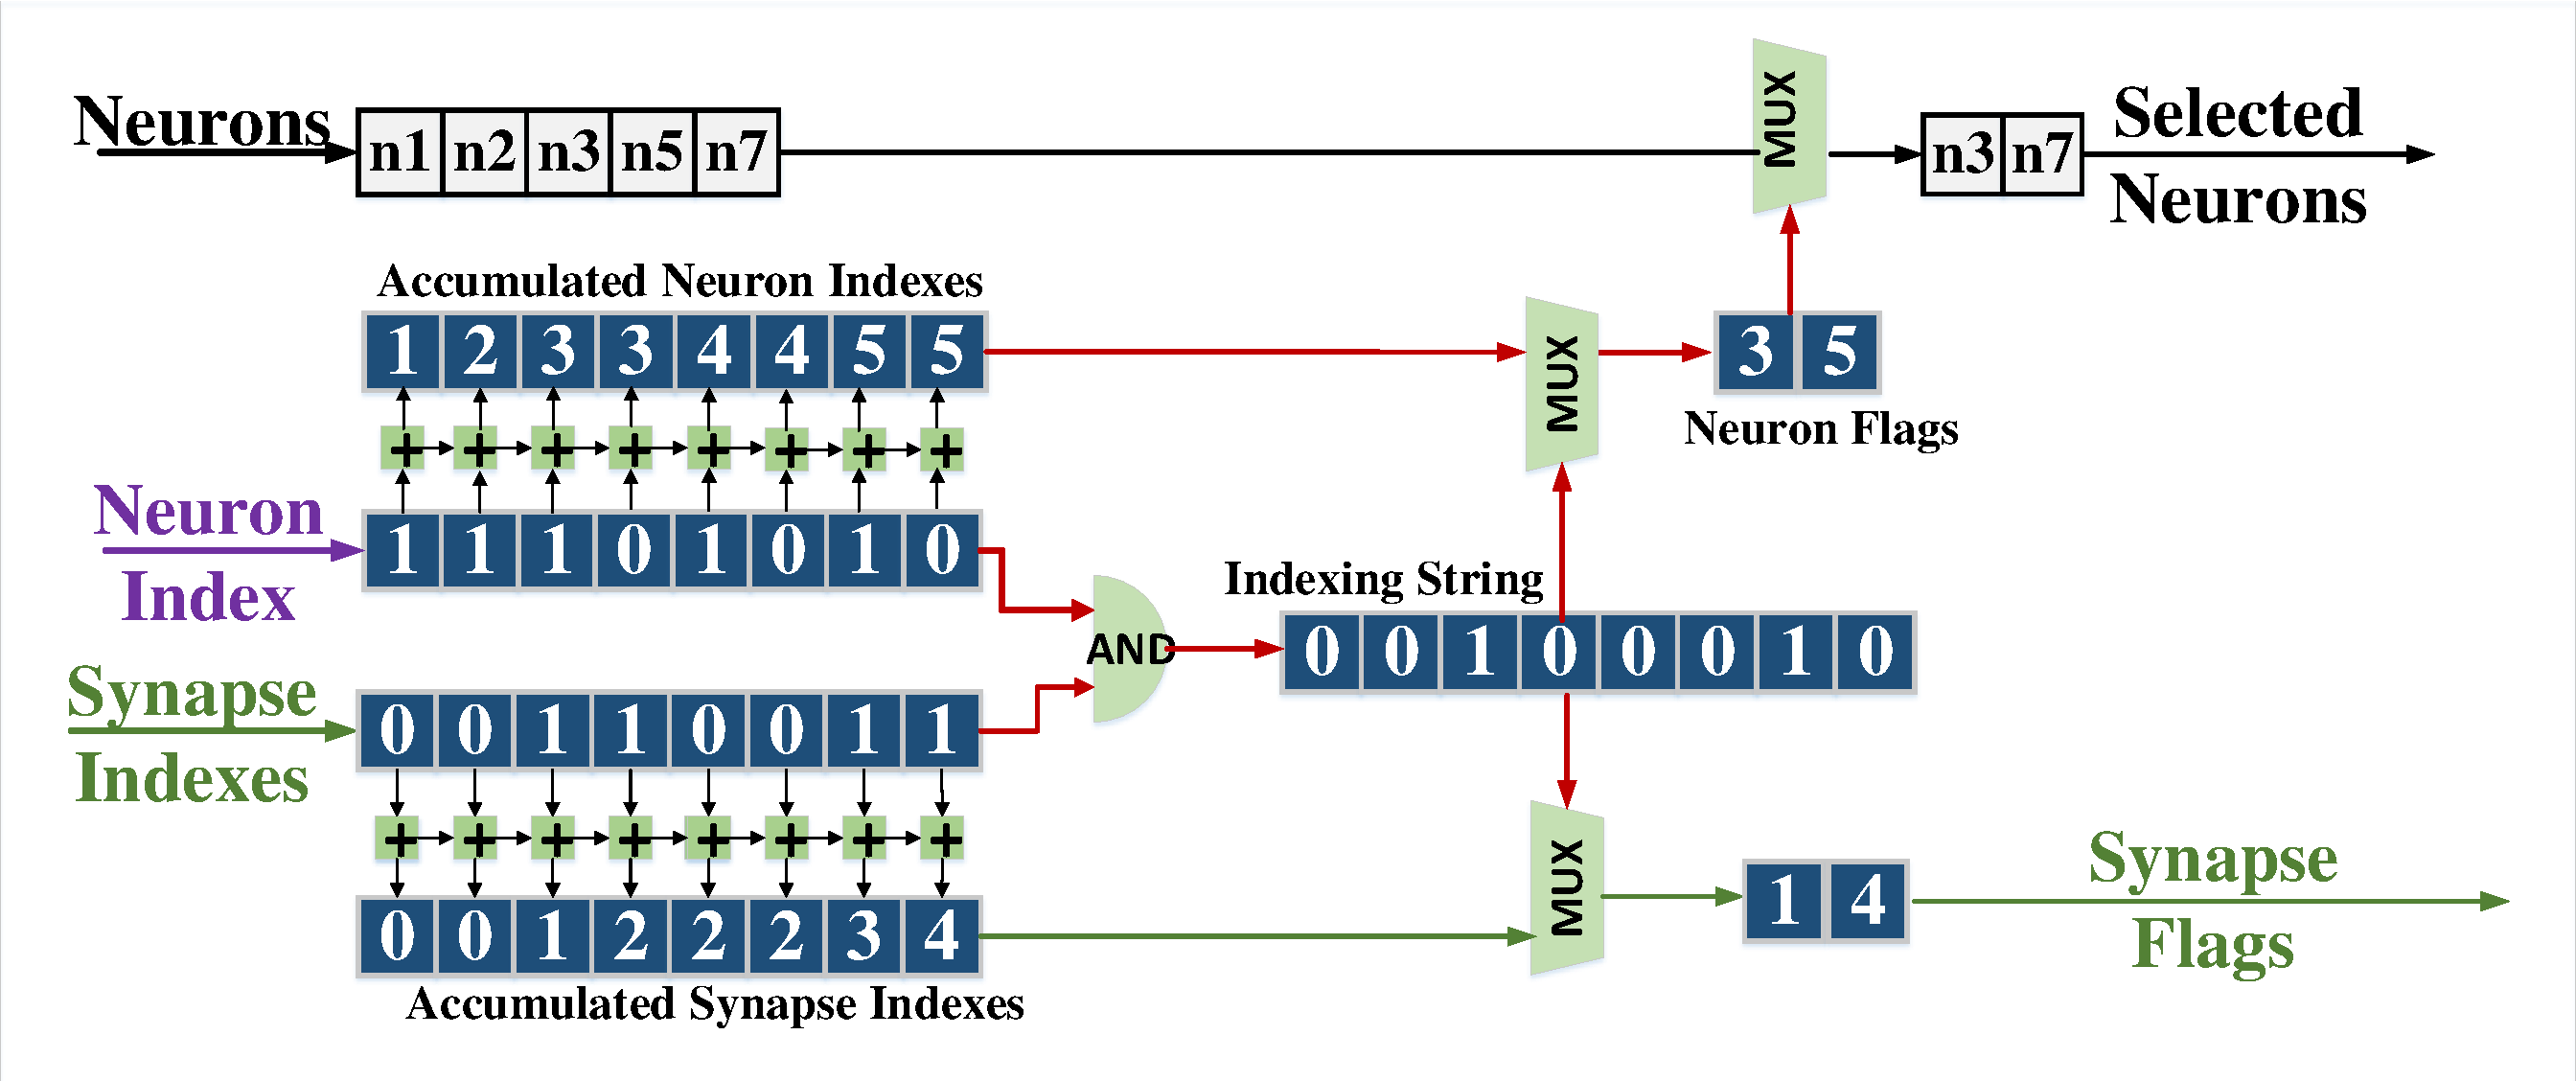
\includegraphics[width=1.0\columnwidth]{NSM.pdf}
\caption{NSM结构}
\label{fig:NSM}
\end{figure}

如图~\ref{fig:NSM}所示,NSM模块的输入为输入神经元,神经元索引和权值索引,NSM模块通过神经元索引和权值索引筛选需要进行计算的输入神经元来处理静态稀疏。为了更有效地利用粗粒度稀疏特性,即多个相邻的输出神经元共享索引和输入神经元,我们设计了一个中心NSM,它能够广播筛选出的神经元信息,从而被多个PE共享。我们利用图~\ref{fig:connection}作为实例来描述NSM筛选输入神经元的流程。
在图~\ref{fig:connection}中的实例中,NSM需要筛从8个输入神经元中筛选出需要进行计算的神经元$n3, n7$并且生成筛选权值需要的synapse flags。具体来说,首先NSM对neuron indexes (~\emph{“11101010”}) 和synapse indexes (\emph{“00110011”}) 执行 “AND” 操作,从而生成indexing string (\emph{“00100010”})。同时neuron indexes和synapse indexes分别累计自身,获得accumulated neuron indexes (\emph{“12334455”}) 和accumulated synapse indexes (\emph{“00122234”}) ,然后分别与indexing string执行 “MUX” 操作,生成neuron flags (\emph{“35”}) 和synapse flags (\emph{“14”})。neuron flags和synapse flags中的数字就表示了需要筛选的神经元和权值的最终位置信息。最后neuron flags与neurons执行 “MUX” 操作筛选出最终需要进行计算的神经元$n3, n7$。值得注意的是,筛选出的神经元与synapse flags被多个输出神经元共享,因此这些信息最后被广播到NFU的各个PE中。最终synapse flags在SSM中被用于筛选出需要进行计算的权值 (见图~\ref{fig:PEFU}(a))。

\subsubsection{NFU}

\begin{figure}[h]
\centering
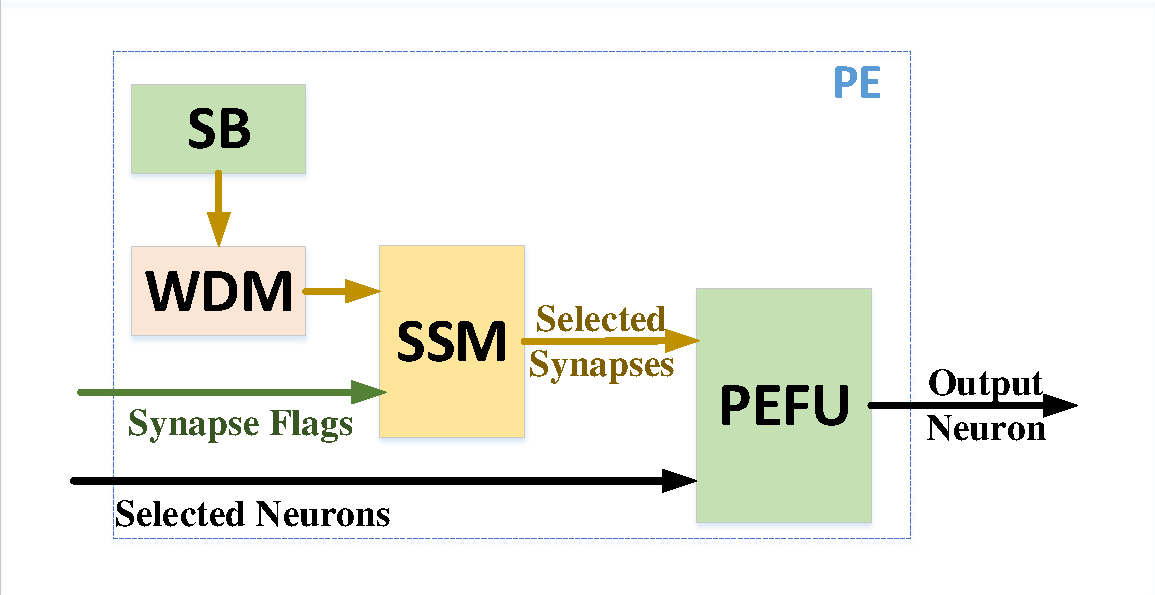
\includegraphics[width=1.0\columnwidth]{PE.pdf}
\caption{PE结构}
\label{fig:PE}
\end{figure}

NFU可以高效地处理神经网络中的所有运算,NFU包含$T_n$个同构的PE来处理动态稀疏性, 同时完成神经网络的运算。如图~\ref{fig:PE}所示,PE由一个局部突触缓冲 (synapse buffer, SB) ,权码解码模块 (weight decoding module, WDM) ,突触选择模块 (synapse select module, SSM) 和处理功能单元 (processing element functional unit, PEFU) 组成。由于每个PE处理共享相同的输入神经元,但是使用独立的权值计算不同的输出神经元,因此我们在每个PE中集成了一个本地的SB,使得每个PE能够从本地SB上加载权值,从而缓减数据传输中的网络拥塞 (network congestion)。同时PE内部集成了一个带有查找表的 (look-up table, LUT) 的WDM,用于处理经过局部量化的权值,提取出实际的权值。SSM接收权值和synapse flags,最终筛选出需要进行计算的权值 (如图~\ref{fig:PEFU}(a))。每个PEFU由$T_m$乘法单元,一个$T_m$输入的加法器树和一个非线性函数模块组成 (如图~\ref{fig:PEFU}(b))。我们使用分时复用的方法将神经网络映射到PE,即每个PE计算一个输出神经元。理想情况下,如果一个输出神经元PE需要$M$个乘法操作,那么PE需要$\lceil M/T_{m} \rceil$个cycle完成计算元,因为PEFU可以在一个cycle内完成$T_m$次乘法。最后,NFU将从$T_n$个PE中收集$T_n$个输出神经元的部分和,传输到NBout中。

\begin{figure}[h]
\centering
\begin{minipage}[b]{0.54\columnwidth}
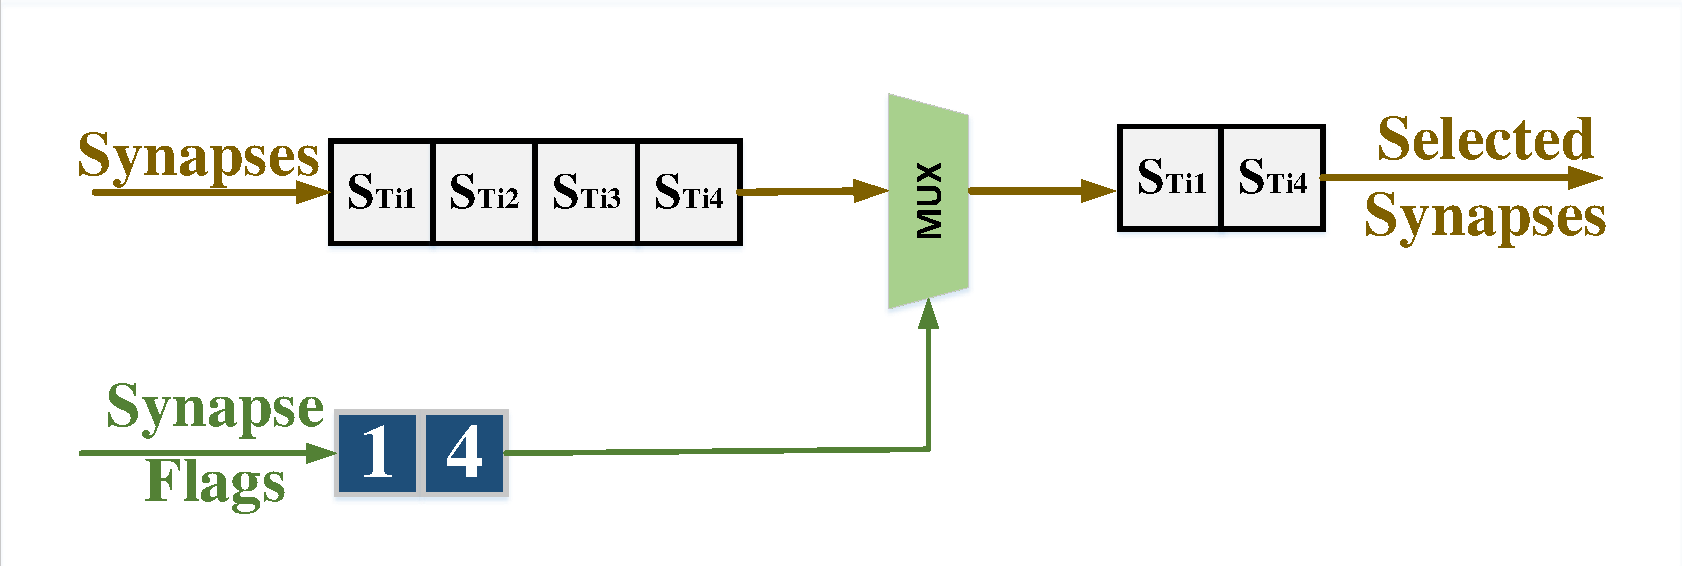
\includegraphics[width=.98\columnwidth]{SSM.pdf}
\end{minipage}
\hfill
\begin{minipage}[b]{0.44\columnwidth}
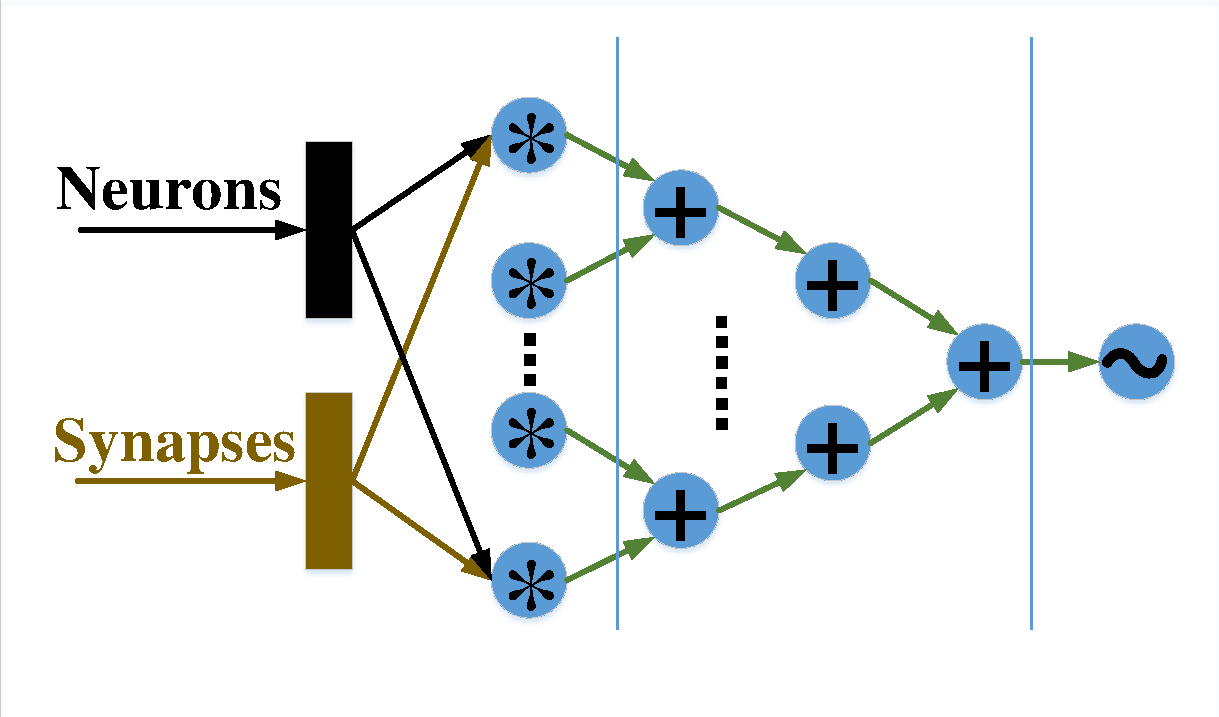
\includegraphics[width=.98\columnwidth]{PEFU.pdf}
\end{minipage}
\caption{(a) SSM结构 (b) PEFU结构}
\label{fig:PEFU}
\end{figure}


SSM用于处理动态稀疏,筛选出需要进行计算的权值。我们采用紧致的形式存储静态稀疏的权值。如图~\ref{fig:connection}所示,对于每个输出神经元,第一个和第四个突触 ($S_{T_{i}1}$ ,$S_{T_{i}4}$) 是计算所需的两个突触。SSM根据NSM产生的synapse flags包含所需突触位置索引 (“14”) 筛选所需的突触。如图~\ref{fig:PEFU} (a)所示,SSM在权值与synapse flags之间执行 “MUX” 操作,最终筛选出需要进行计算的权值。由于每个PE接收不同的权值,并且处理不同的输出神经元,我们在每个PE内部局部集成SSM和SB,从而避免高带宽和长延迟。

\subsubsection{Encoder}

\begin{figure}[h]
\centering
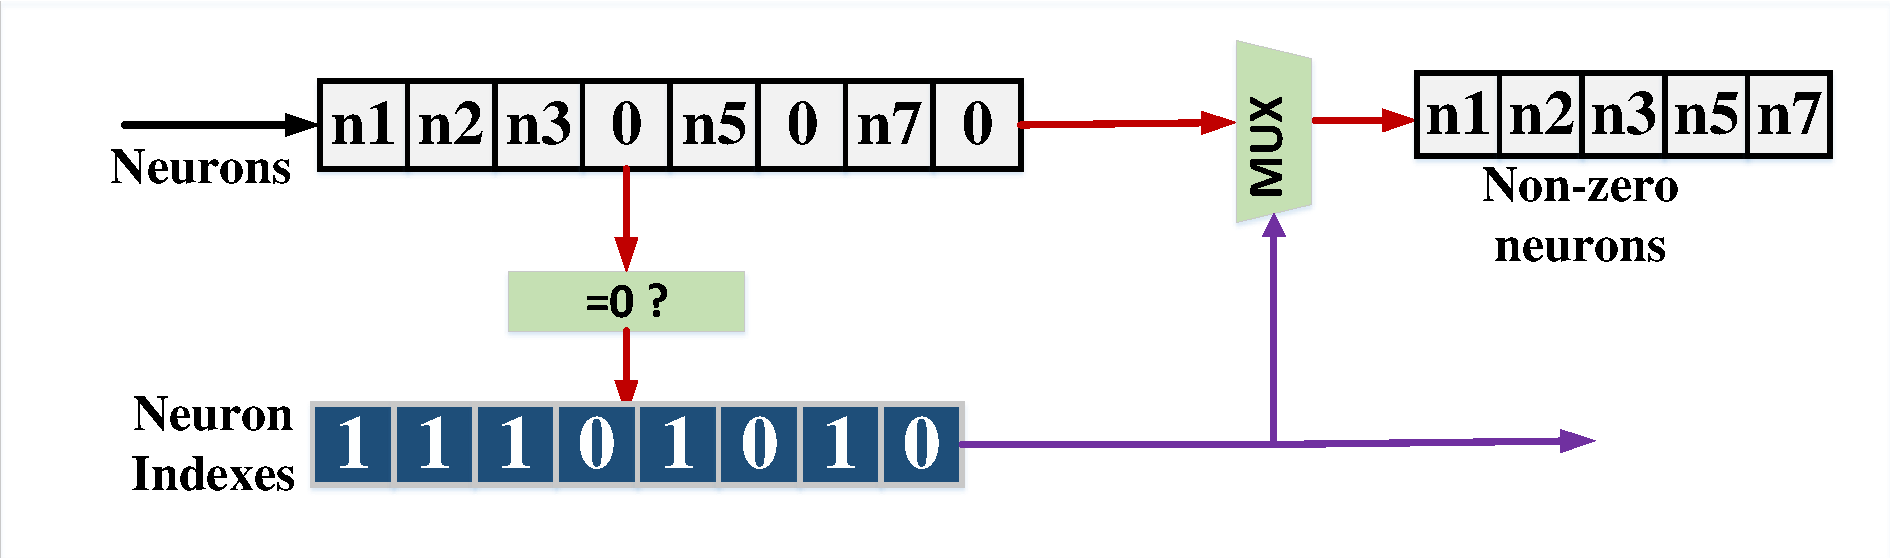
\includegraphics[width=1.0\columnwidth]{encoder.pdf}
\caption{Encoder架构}
\label{fig:encoder}
\end{figure}

图~\ref{fig:encoder}展示了神经元压缩模块Encoder的架构。Encoder模块与Nbout直接相连,用于消除输出神经元中的零元素,最终稀疏的神经元使用非零神经元和比特串进行表示。具体来说,Encoder根据神经元的激活值,生成synapse indexes (“11101010”),每个索引指示相应的神经元激活是否为零。然后Encoder在神经元与synapse indexes之间执行 “MUX” 操作筛选出非零的神经元。最终非零神经元与对应的索引synapse indexes被传输到片外,然后作为下一层网络的输入被重新加载到NBin。通过动态压缩神经元,加速器能够显著减少DRAM访问神经元的开销,从而减少DRAM的访存能耗。

\subsection{存储模块}
\label{subsec:storage}

考虑到不同数据在加速器中的不同行为模式,我们将偏上缓存分为三个部分:一个输入神经元缓存(NBin),一个输出神经元缓存(NBout)和$T_m$个权值缓存(SB),考虑到神经元稀疏和权值稀疏的情况,我们增加了两个索引缓存,分别是输入神经元索引缓存(NIBin)和权值索引缓存(SIB)。为了实现数据的高速流水,我们使用乒乓(ping-pong)的模式管理所有的缓存。

对于NBin,我们设置带宽为$16\times T_m \times 16$比特,设置这个带宽主要是考虑到PE的利用率。虽然PE共享相同的输入神经元,但是每个PE在一个cycle需要$T_m$个输入神经元来避免PEFU中计算单元的空转。考虑到现有大部分神经网络的稠密度都高于$1/16$(即稀疏度低于$15/16$),特别是卷积层,一般稠密度为$30\%$左右,因此,我们在一个cycle发送给NSM$16\times T_m$个输入神经元时,就能够保证NSM在一个cycle能够筛选出$T_m$个输入神经元,从而保证PEFU的运行效率。

对于NBout,我们设置其带宽为$4\times T_n \times 16$比特,这部分主要是考虑到动态神经元稀疏。如表~\ref{tab:sparsities}考虑到现有大部分神经网络的神经元稠密度高于$25\%$(即稀疏度低于$75\%$),当我们在每一个cycle发送给Encoder$4\times T_n$个输出神经元时,就能够保证Encoder在一个cycle筛选出$T_n$个神经元进行压缩,从而保证流水顺利进行。

对于每一个PE中的SB,我们设置带宽$4\times T_m\times 16$比特,保证能够在一个cycle读取$4\times T_m$个权值。考虑到现有大部分神经网络的动态稀疏度低于$75\%$,$4\times T_m \times 16$比特的带宽能够保证SSM在一个cycle筛选出$T_m$个权值,从而保证PEFU的运行效率。由于权值是以压缩形式(通过剪枝和局部量化)存储在SB中,局部量化会导致权值在不同的神经网络和不同层中的位宽不同,例如,在AlexNet网络的卷积层中权值被量化为8比特,在MLP网络的全连接层中权值被量化为6比特,在AlexNet网络的全连接层中权值被量化为4比特。不同的量化比特会导致WDM模块庞大的面积/功耗开销,因此我们将权值按照4比特进行对齐操作。例如,假设SRAM的一行为128比特,那么当权值被量化为16比特,8比特和4比特时,SRAM的一行分别能够存储8个,16个和32个权值。因此,$T_m \times 64$比特的权值能够被WDM解码成为$T_m \ times 16$个权值(当权值被编码成小于或者等于4比特),或者$T_m \times 8$个权值(当权值被编码成大于4比特而小于等于8比特),或者$T_m \time 4$个权值(当权值被编码成大于8比特,小于等于16比特)。对比于支持所有位宽编码形式的解码模块,我们的WDM能够减少5.14倍的面积和4.27的功耗。

对于NIBin和SIB,我们设定其宽度为$16\times T_m\times 1$比特,因为我们使用直接索引的方式存储稀疏的神经元和权值,索引中的每一比特用于表示对应的元素是否为“0”表明是否存在相应的突触。因此,NIBin和SIB则需要$16\times T_m\times 1$比特的带宽与Nbin提供给NSM的$16\times T_m$个输入神经元一一对应。

五个缓存的大小决定了整个架构的整体性能和能耗。尽管有部分研究~\cite{chen2014dadiannao,han2016eie}提出,加速器需要提供足够大的缓存来保存神经网络所有的权值和神经元从而避免昂贵的片外访存开销,但是这种设计会大大增加延迟,面积,功耗;同时这种设计方案缺少可扩展性,并不能很好地支持新兴的规模更大,层数更深的神经网络。因此我们使用小的缓存以及适当的数据替换策略,从而权衡加速器的可扩展性,性能和能耗。在探索了不同大小的缓存区后,我们设定NBin,NBout,SB,SINin和SIB的大小分别是$8KB$,$8KB$,$32KB$,$1KB$和$1KB$。

\subsection{控制}

\begin{figure}[h]
\centering
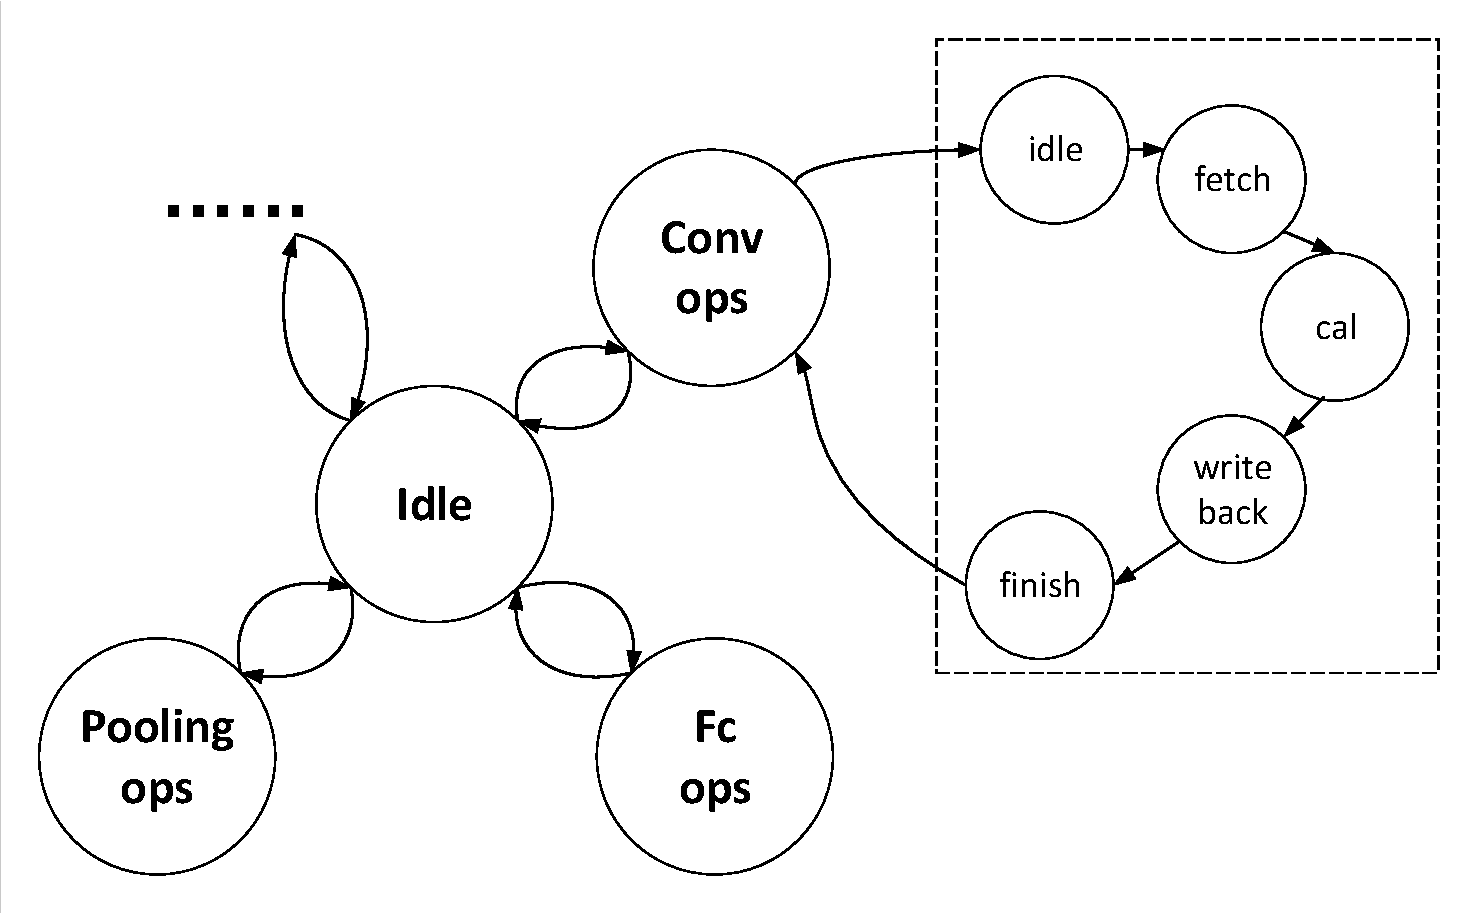
\includegraphics[width=0.8\columnwidth]{FSM.pdf}
\caption{CP的有限状态机}
\label{fig:FSM}
\end{figure}

CP用于控制加速器的整个执行流程。它从内部指令缓存中读取指令然后进行解码,从而有效地协调数据组织,数据访问和数据计算的过程。CP通过监控各个模块对应的控制寄存器来监控每个模块的状态。同时我们利用基于库的编译器生成高效的超长指令字(Very Long Instruction Word,VLIW)。同时,我们为CP设计了高效的有限状态机(finite state machine, FSM),如图~ref{fig:FSM}所示。FSM分为两层控制状态,第一层状态表示神经网络中的宏观操作,如卷积,内积,池化,激活等操作;第二层状态则是每一个宏观操作中的细节,如对于卷积操作还会有数据预取,计算,写回等不同的状态。

\subsection{片上互联}

\begin{figure}[h]
\centering
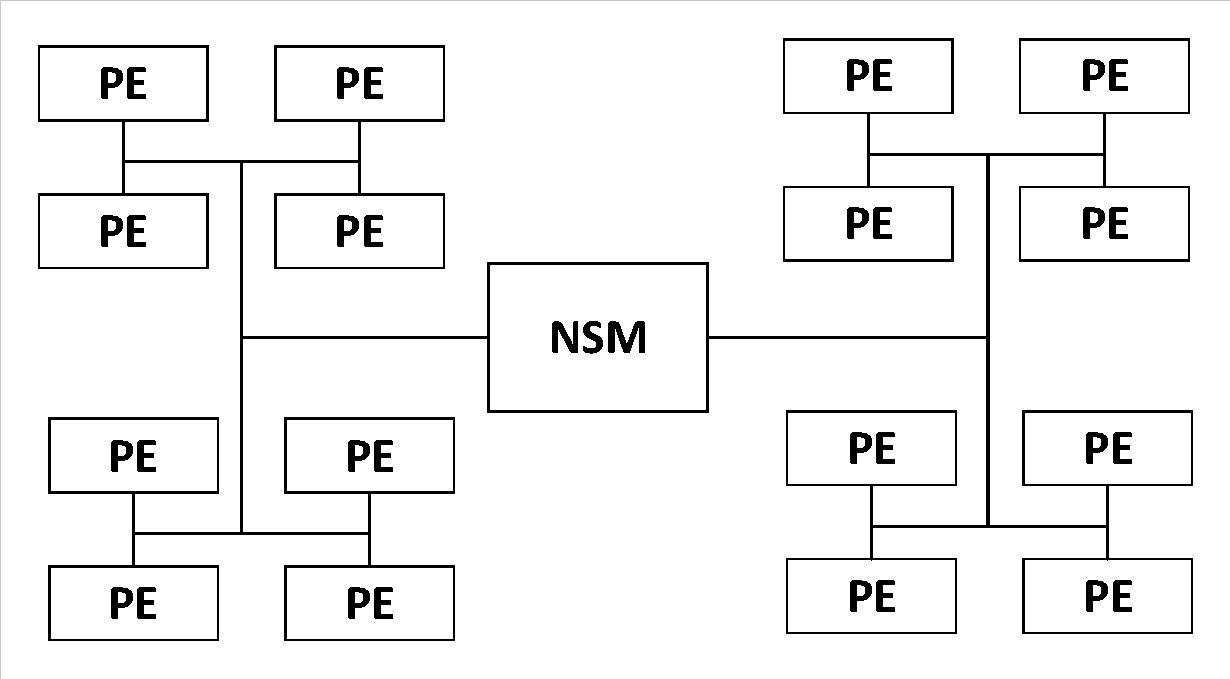
\includegraphics[width=0.8\columnwidth]{Htree.pdf}
\caption{H树互联结构}
\label{fig:Htree}
\end{figure}

如图~\ref{fig:Htree}所示,我们采用H树的拓扑结构连接NSM与NFU中的$T_n$个PE。由于NSM产生的selected neurons和synapse flags被所有PE共享,而且PE之间的负载是一种均衡的状态,因此NSM通过H树将这些信息通过广播的形式传送给PE,从而避免NSM和PE之间由于距离差异引起的不平衡延迟的问题;同时H树拥有非常良好的可扩展性,能够非常方便地对PE进行扩展,在不改变整体拓扑结构的情况下通过增加PE的数量增加加速器的计算能力,从而应对更大规模的神经网络。

\section{编程模型}

\subsection{基于库的编程模型}
考虑到实际应用场景和开发效率,高级编程模型,如Caffe~\cite{jia2014caffe},Tensorflow~\cite{abadi2016tensorflow}, MXNet~\cite{chen2015mxnet}等为用户提供了一系列C++的库函数接口,使得用户能够方便地调用这些接口,从而控制CPU或者GPU完成神经网络的运算。高级编程模型能够大幅度增加用户或者开发人员的编程效率,特别是算法和应用程序开发人员。因此,专用的加速器必须为用户提供类似于高级编程框架的接口,以减轻用户的编程负担。为此,我们提供了基于库的编程模型,其基本思想是为用户提供一系列C++的高级库函数接口,每一个函数对应了神经网络中一个基本操作,如卷积运算,内积,池化等操作。代码~\ref{list:conv}就是卷积层库函数的接口,用户首先通过TensorDescriptor和FilterDescriptor定以卷积操作涉及输入/输出和权值;同时分别使用setTensorDescriptor和setFilterDescriptor分别描述输入/输出和权值的特性,如稀疏,大小,地址等。然后用户通过ConvDescriptor和setConvDescriptor分别定义卷积操作描述符和卷积操作的特性,如输入/输入/权值规模,步长,padding等。最后用户调用convForward执行卷积操作。用户通过调用这个库函数接口能够非常方便地最终驱动加速器完成卷积操作。

\begin{lstlisting}[language=C, frame=single, basicstyle=\footnotesize, caption=卷积层库函数接口, label=list:conv, captionpos=b]
  // Data Declaration
  TensorDescriptor input, output;
  FilterDescriptor weight;
  setTensorDescriptor(input, ...);
  setTensorDescriptor(output, ...);
  setFilterDescriptor(weight, ...);
  // Operations
  ConvDescriptor conv;
  setConvDescriptor(...);
  ConvForward(conv, input, weight, output);
\end{lstlisting}

我们将库嵌入到深度学习框架Caffe中,如图~\ref{fig:framework}所示,这一套编程框架对用户完全透明,使得用户能够无缝使用我们的加速器。值得注意的是我们需要为我们的加速器设计专用的编译器(compiler),使其能够将C++源码编译成为加速器中的可执行指令。

\begin{figure}
\centering
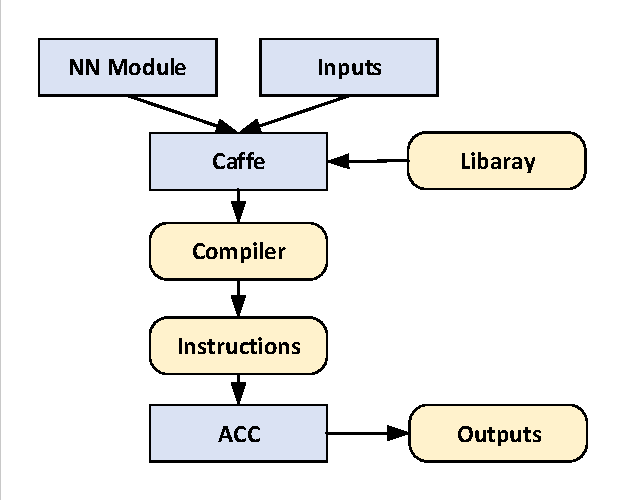
\includegraphics[width=0.6\columnwidth]{framework.pdf}
\caption{编程框架}
\label{fig:framework}
\end{figure}

\subsection{编译器}
深度学习框架(如caffe)与我们的加速器之间存在巨大的鸿沟,如何为加速器建立一套完整的编程生态系统是一个巨大的挑战。为此我们需要为加速器设计专用的基于库的编译器,从而将基于库的源文件编译成为加速器中可执行指令。编译的主要挑战来源于加速器中复杂的片上数据管理。

具体来说,第一,神经网络中的数据多样性和特征多样性增加了数据分配和数据搬运的复杂度。由于神经网络中有不同类型的参数,如输入/输出神经元,权值等;同时不同的数据拥有不同的特征,如神经元有动态稀疏的特性,权值有静态稀疏和量化的特性。如何根据数据的特征为不同的数据种类分配数据空间,如何搬运不同种类的数据成为一个巨大挑战,因此,我们为不同的数据使用适当的数据分配和数据搬运策略来提升效率。

第二,有限的片上缓存(\ref{subsec:storage})增大了数据调度的复杂性。考虑到神经网络中庞大的神经元/突触的和加速器中有限的片上内存之间的矛盾,我们需要使用loop tiling对数据进行切分,同时使用合适的数据重用策略提升加速器的性能。而不同的loop tiling策略和数据重用 (data reuse) 策略会进一步影响片外数据访问,片上数据访问,计算调度,从而影响加速器的效率和性能。因此我们需要在编译期间探索不同的loop tiling策略和数据复用策略,选择最优的loop tiling方式和最佳的数据服用策略,最大程度挖掘加速器的性能。

\begin{figure}[h]

\centering
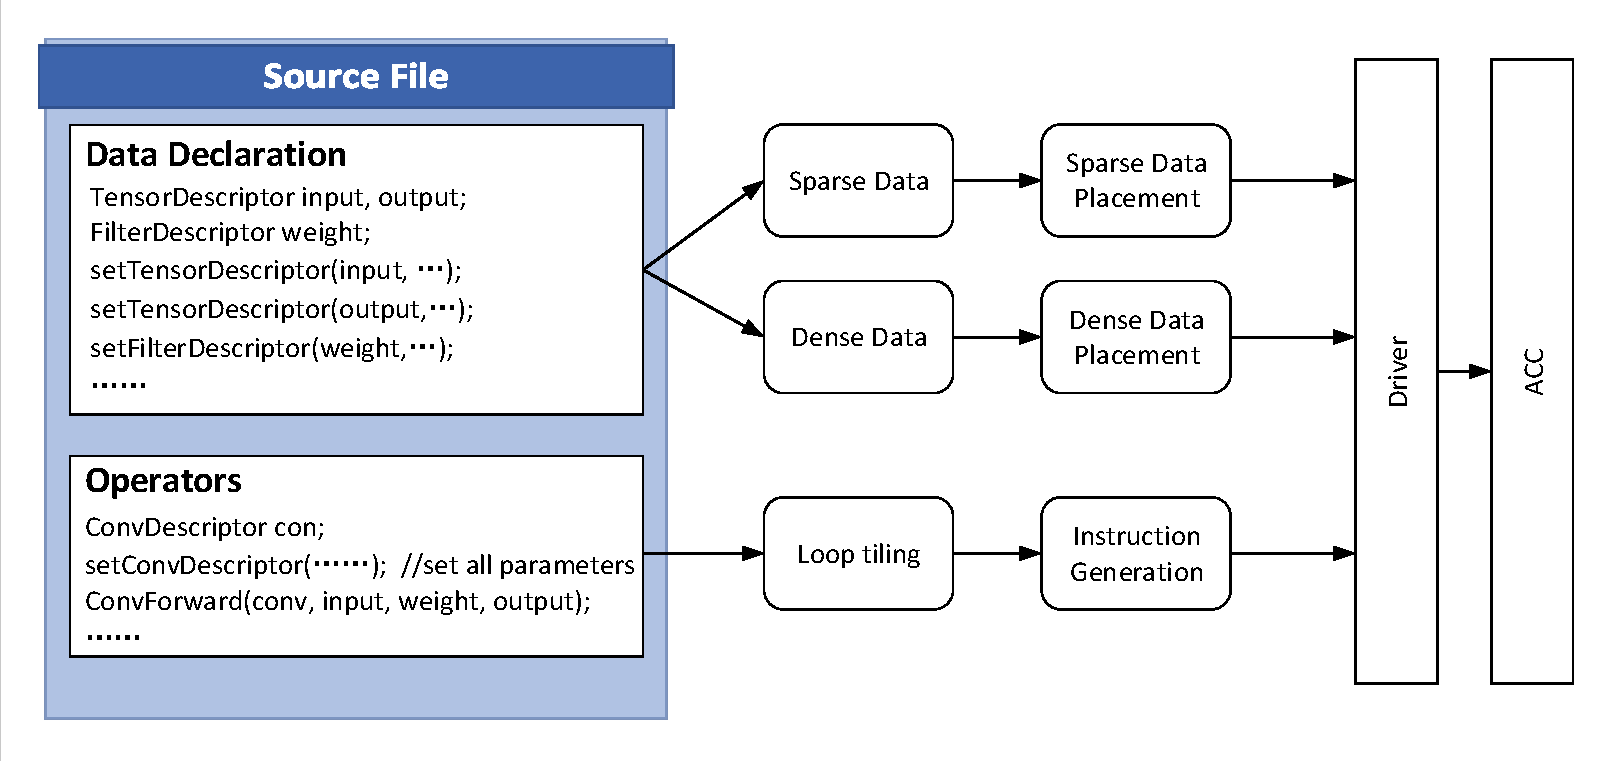
\includegraphics[width=1.0\columnwidth]{compiler.pdf}
\caption{源文件编译成为加速器可执行代码的过程}
\label{fig:compiler}
\end{figure}

我们设计为加速器设计了一个专用的编译器来弥合深度学习框架与加速器之间的差距。如图~\ref{fig:compiler}所示,我们显示了如何将基于库的源文件编译成为加速器的可执行代码。编译过程分为两个阶段:数据摆放(data placement)和指令生成(instruction generation)。

在数据摆放阶段,源代码中的数据结构被合理地分配到加速器的片上缓存中。我们使用张量(tensor)对输入和输出神经元进行封装,同时我们用过滤器(filter)对权值进行封装,值得注意的是,tensor和filter都是四维的张亮。我们使用不同的数据结构封装不同数据类型,是因为不同类型的数据会被分配到加速器不同的片上缓存中(如输入神经元,输出神经元和权值会分别被分配到NBin,NBout和SB中)。同时考虑到数据稀疏的特性,我们使用sparse这个枚举类型作为描述符添加到tensor(动态稀疏)和filter(静态稀疏)的属性中。

在指令生成阶段,我们使用加速器专用运算操作(如卷积操作,池化操作等)对数据进行运算操作,同时我们使用loop tiling将这些操作分解为子操作,以确保子操作对应的数据能够(即输入/输出神经元,权值)能够填充到有限的片上缓存中。值得注意的是,在指令生成阶段,数据搬运操作将与数据运算操作同时生成。最后,代码生成器将这些操作转换成为可执行的指令,使得其能够在加速器上解码和执行。


\subsection{loop tiling}

Loop tiling能够对计算进行合理划分,以确保子计算所涉及的数据能够被完全填充到片上缓存中。由于片外访存会花费巨大的能耗(占用超过$90\%$的整体能耗),因此loop tiling策略优先考虑如何提高片上数据重用性,从而减少片外数据访存,从而减少加速器的访存能耗。Eyeriss~\cite{chen2017eyeriss}提出了四种不同的数据重用策略,分别是卷积重用(\emph{convolutional reuse}),卷积核重用(\emph{filter reuse}),输入特征图重用(\emph{input feature map reuse})和部分和重用(\emph{partial sums reuse})。考虑到我们的加速器与Eyeriss架构上的差异,我们将数据重用策略分为三种类型,即输出重用(\emph{output-reuse}, 与Eyeriss中的\emph{partial sums reuse}对应),突触重用(\emph{synapse-reuse},与Eyeriss中的\emph{convolutional reuse}和\emph{filter reuse}对应)和输入重用(\emph{input-reuse},与Eyeriss中\emph{input feature map resue}对应);这三种策略分别表示最大程度重用输出部分和数据,突触数据和输入数据。对于\emph{output-reuse}策略,在运算过程中,一段输入神经元被加载到NBin中,一段权值被加载到SB中,然后计算出一段输出神经元的部分和,然后将其存储到NBout中;在下一个阶段,第二段的输入神经元和权值被加载到片上缓存持续计算NBout中输出神经元部分和,这个过程一直循环直至NBout中的这一段输出神经元被完全计算完成,最后NBout中的输出神经元被存储到片外;因此在\emph{output-reuse}策略中,输入神经元和权值会多次从片外加载到片上缓存,而输出神经元会持续存储在片上缓存中直至被完全计算完成。同理,在\emph{synapse-resue}策略中,输入神经元和输出神经元会被多次从片外加载到片上,直至片上的权值被完全重用。在\emph{input-reuse}策略中,权值和输出神经元会被多次从片外加载到片上,直至片上的输入神经元被完全重用。因此我们在编译阶段需要探索最佳的数据重用策略,减少片外访存的能耗。

不失一般性的,我们以VGG16网络的\emph{conv4\_2}卷积层为例,来计算不同的数据重用策略对片外访存的需求。具体来说,\emph{conv4\_2}的输入规模为$30\times 30\times 512$(考虑到输入需要进行padding),权值的规模为$32\times 32\times 512\times 512$, 输出的规模为$28\times 28\times 512$,其中输入神经元和权值的稠密度分别是$40.52\%$(稀疏度为$59.48\%$)和$34.20\%$(稀疏度为$65.80\%$)(如表~\ref{tab:sparsities}所示)。加速器中NBin,SB和NBout的大小分别是$8KB$,$8KB$和$32KB$。在loop tiling过程中,我们将数据且分为$SegN$块,其中每一块数据量为$SegSize$。为了尽可能提高片上缓存的利用率,我们将输出的channel维度按照$4\times 128$($SegN\times SegSize$)的方式进行切分,在height维度按照$28\times 1$的方式进行切分;同时我们将输入的channel方向按照$16\times 32$的方式进行切分。经过loop tiling后,输入,权值,输出每一个数据块的大小分别为$SegSize_{in} = 30\times 3\times 32\times 40.52\%$, $SegSize_{syn} = 3\times 3\times 32\times 128\times 34.20\%$ 和 $SegSize_{out} = 28\times 1\times 128$。值得注意的是,我们对输入数据块和权值数据块分别乘以网络的稠密度来进行近似。因此,使用~\emph{input-reuse},\emph{output-reuse}和\emph{synapse-reuse}策略,所需要的片外访存的开销可以按照如下公式进行计算
\begin{gather*}
MEM_{i} = 16 \times 1 \times 28 \times (SegSize_{in} + SegSize_{syn} \times 4 + SegSize_{out} \times 4 \times 2)\times 2 = 68.59MB \\
MEM_{o} = 4 \times 28 \times 1 \times (SegSize_{out} + SegSize_{in} \times 16 + SegSize_{syn} \times 16)\times 2 = 47.85MB \\
MEM_{s} = 16 \times 4 \times (SegSize_{syn} + SegSize_{in} \times 28 \times 1 + SegSize_{out} \times 28 \times 2)\times 2 = 30.03MB 
\end{gather*}
因此我们为\emph{conv4\_2}卷积层选择\emph{synapse-reuse}的策略。


\section{Discussion}








\chapter{实验方法和实验结果}

\zadd{本章首先介绍实验方法,包括实验工具链,实验平台和benchmark。然后介绍和分析实验结果,包括硬件属性分析,性能分析和能耗分析。最后我们对加速器的一些特性,如熵编码/解码,稀疏利用率等进行深入讨论。
}

\section{实验方法}
在本节中,我们介绍Cambricon-S相关的实验方法。

我们使用Synopsys工具链中的TMSC $65nm$库对加速器的RTL实现进行综合。我们使用CACTI 6.0预测DRAM访存能耗~\cite{muralimanohar2007optimizing}。我们使用基于PrimeTime PX的VCD波形文件评估能耗。最后我们使用基于事件触发的模拟器评估加速器的性能。

\subsection{Baseline}
我们将Cambricon-S与CPU,GPU和硬件加速器进行比较。

\subsubsection{CPU}
我们使用目前流行的深度学习框架Caffe~\cite{jia2014caffe}评估神经网络在CPU上的性能。CPU的型号是拥有6核的英特尔志强 E5-2620 v2,工作频率为$2.1GHz$,工艺为$22nm$。同时,我们使用稀疏库(sparse-BLAS)~\cite{duff2002overview}来评估稀疏神经网络的性能。我们用CPU-Caffe和CPU-Sparse分别表示稠密网络和稀疏网络在CPU上的性能。

\subsubsection{GPU}
我们使用Caffe评估神经网络在GPU上的性能(用GPU-Caffe表示)。GPU的型号是Nvidia K20,拥有$5GB$ GDDR5,峰值能够达到$3.52TFlops$,工艺为$28nm$。同时我们使用cuBLAS来实现神经网络算法(用GPU-cuBLAS表示)。最后,我们使用先进的cuSparse库评估稀疏神经网络的性能(用GPU-Sparse表示)。

\subsubsection{硬件加速器}
我们将新型加速器与目前最先进的神经网络加速器DianNao和Cambricon-X进行性能比较。DianNao拥有很高的吞吐量,能够加速大多数的CNN和DNN。Cambricon-X是一个稀疏神经网络加速器,它能够利用稀疏特性提高性能同时降低能耗。我们选择Cambricon-X作为baseline,主要是考虑到它能够最大程度利用稀疏特性,并且具有通用性。考虑到稀疏利用率,对比稠密神经网络,Cambricon-X通过挖掘稀疏性能够获得2.93倍的加速比,而Cnvlutin和SCNN分别只能获得1.37倍和2.7倍的加速比。考虑到通用性,SCNN在全连接层上的性能非常低,而EIE只能用来加速稀疏的全连接层。

\subsection{Benchmark}
如表~\ref{tab:compression}所示,我们使用七个代表神经网络:AlexNet, VGG16, LeNet-5,MLP,Cifar10,ResNet152和LSTM作为benchmark。值得注意的是,我们表中参数都是经过粗粒度剪枝后的网络参数。

\section{实验结果}

\subsection{硬件属性}

在当前的加速器中,为了兼容剪枝块的大小,我们将PE的数量$T_n$以及每个PE内部乘法器数量$T_m$配置为$T_n = T_m = 16$,同时考虑到神经网络神经元和权值的稀疏度,我们将NSM设计为256选16的结构,SSM设计为64选16的结构,Encoder设计为64选16的结构。新型加速器的布局特点,各模块的面积和功耗如表~\ref{tab:hardware}所示。加速器的总面积和总功耗分别是$6.82mm^2$和$821.19mW$,工作频率为1GHz,吞吐量为512GOP/s,片上SRAM共为$54KB$。新型加速器的面积分别是Cambricon-X($6.38mm^2$)和DianNao($3.02mm^2$)的1.07倍和2.26倍,同时功耗比Cambricon-X($954mW$)低$132.81mW$,比DianNao($485mW$)高$336.19mW$。
值得注意的是,我们当前加速器并不包含熵解码模块,因此不支持经过熵编码后的神经网络。

\begin{table}[h]
\caption{加速器详细属性}
\centering
\label{tab:hardware}
\begin{tabular}{lllllllllllll}
\toprule
 & Area($mm^2$) & \% & Power(mW) & \% \\
\midrule
Total   & 6.82	& 100.00\% 	& 821.19    & 100.00\% \\
\midrule
NBin    & 0.55  & 8.06		& 93.32     & 11.36	\\
NBout   & 0.55  & 8.06	    & 93.32     & 11.36	\\
SIB     & 0.05 	& 0.73		& 6.89      & 0.84	\\
NIB     & 0.05  & 0.73      & 6.89      & 0.84  \\
CP      & 0.16 	& 2.35		& 75.06     & 9.14	\\
NSM     & 0.69 	& 10.12		& 121.46    & 14.79	\\
Encoder & 0.04  & 0.60      & 15.75     & 1.92  \\
NFU     & 4.73 	& 69.35 	& 408.50    & 49.75	\\
~~~SB   & ~~~1.05 	& ~~~22.20	& ~~~151.91 & ~~~37.19\\
~~~SSM  & ~~~0.25 	& ~~~5.29	& ~~~56.80  & ~~~13.90	\\
~~~WDM  & ~~~1.54 	& ~~~32.56	& ~~~16.25  & ~~~3.98	\\
~~~PEFU & ~~1.89	& ~~~33.95	& ~~~183.54 & ~~~44.93 \\
\bottomrule
\end{tabular}
\end{table}

此外,Cambricon-S中处理稀疏和量化模块(NSM, SSMs, Encoder和WDM)的面积和功耗分别是$2.52mm^2$(占总面积的$36.95\%$)和$210.26mW$(占总功耗的$25.60\%$),却能够获得比Cambricon-X高的1.71倍性能,同时降低1.75倍的能耗。值得注意的是,即使新增了突触选择模块,新型加速器的索引模块(即NSM和SSM)的面积对比与Cambricon-X的IM模块减少了2.11倍($0.94mm^2$ vs. $1.98mm^2$),功耗减少了1.87 倍($178.26mW$ vs. $332.62mW$);同时新型加速器的NSM的面积和功耗分别是Cambricon-X中IM模块的$36.52\%$和$34.85\%$,却实现了与IM模块相同的功能(即筛选神经元)。因此,我们的设计对比于Cambricon-X在面积,能耗上都有很大的提升。

\subsection{性能}
在表~\ref{tab:compression}所列出的七个benchmark上,我们比较了Cambricon-S,CPU,GPU,DianNao和Cambricon-X的性能。在CPU和GPU上,我们同时评估稀疏神经网络和稠密神经网络的性能,即我们使用稀疏库(CPU-Sparse,GPU-Sparse)评估稀疏神经网络的性能,使用稠密库(CPU-Caffe, GPU-Caffe, GPU-cuBLAS)评估稠密神经网络的性能。为了与CPU和GPU公平比较,我们评估了加速器在稠密网络上的性能(ACC-dense)。同时为了与Cambricon-X和DianNao公平比较,我们评估了这三个加速器在稀疏神经网络上的性能。

\begin{figure}[h]
\centering
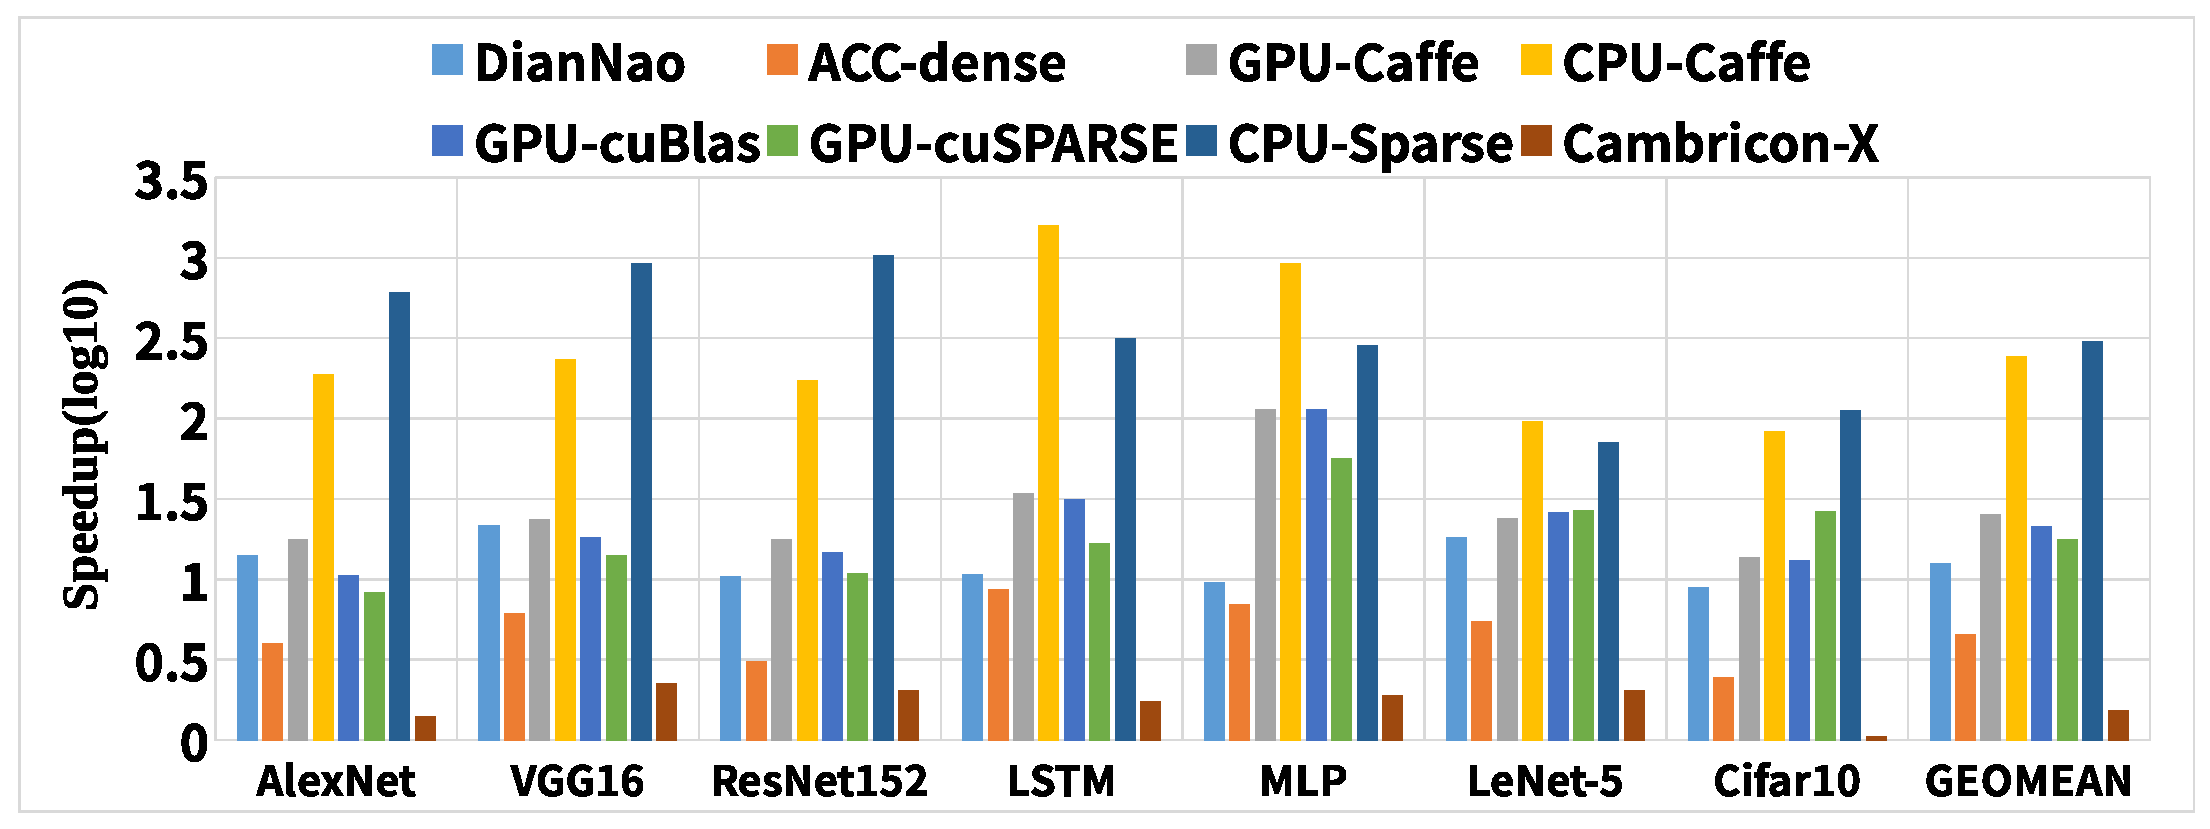
\includegraphics[width=0.8\columnwidth]{total_performance.eps}
\caption{Cambricon-S与CPU,GPU,DianNao,Cambricon-X的性能对比}
\label{fig:total_performance}
\end{figure}

在图~\ref{fig:total_performance},我们比较了Cambricon-S,CPU,GPU,DianNao和Cambricon-X的性能,同时,我们将所有性能的数据归一化到了Cambricon-S在稀疏网络上的性能。在稠密网络上,Cambricon-S与CPU-Caffe,GPU-Caffe和CPU-cuBLAS对比分别能够获得44.8倍,5.8倍和5.1倍的加速比。在稀疏网络上,Cambricon-S与CPU-Sparse和GPU-cuSparse对比分别能够获得331.1倍和19.3倍的加速比。对比于DianNao和Cambricon-X,Cambricon-S分别能够获得13.10倍和1.71倍加速的加速比。实验结果充分显示了我们的加速器能够充分利用利用神经网络稀疏的特性,从而获得高加速比。值得注意的是,我们的加速器能够通过关闭/开启各个模块(NSM,SSM,WDM,Encoder等),使得加速器能够处理稠密神经网络,稀疏神经网络(包括只利用权值稀疏,只利用神经元稀疏和同时利用神经元/权值稀疏三种情况),局部量化。

为了进一步探索Cambricon-S的性能,我们统计了Cambricon-S在卷积层和全连接层上的性能。如图~\ref{fig:conv_performance}所示,在卷积层上,对比于CPU-Sparse, GPU-cuSparse和DianNao,我们的加速器分别获得了283.31倍,12.20倍和13.94倍的性能提升。如图~\ref{fig:fc_performance}所示,在全连接层上,对比于CPU-Sparse, GPU-cuSparse和DianNao,我们的加速器分别获得了531.89倍,79.05倍和13.56倍的性能提升。值得注意的是,对比于Cambricon-X,Cambricon-S能够在卷积层和全连接层分别获得1.66倍和2.15倍的加速比。

\begin{figure}[h]
\centering
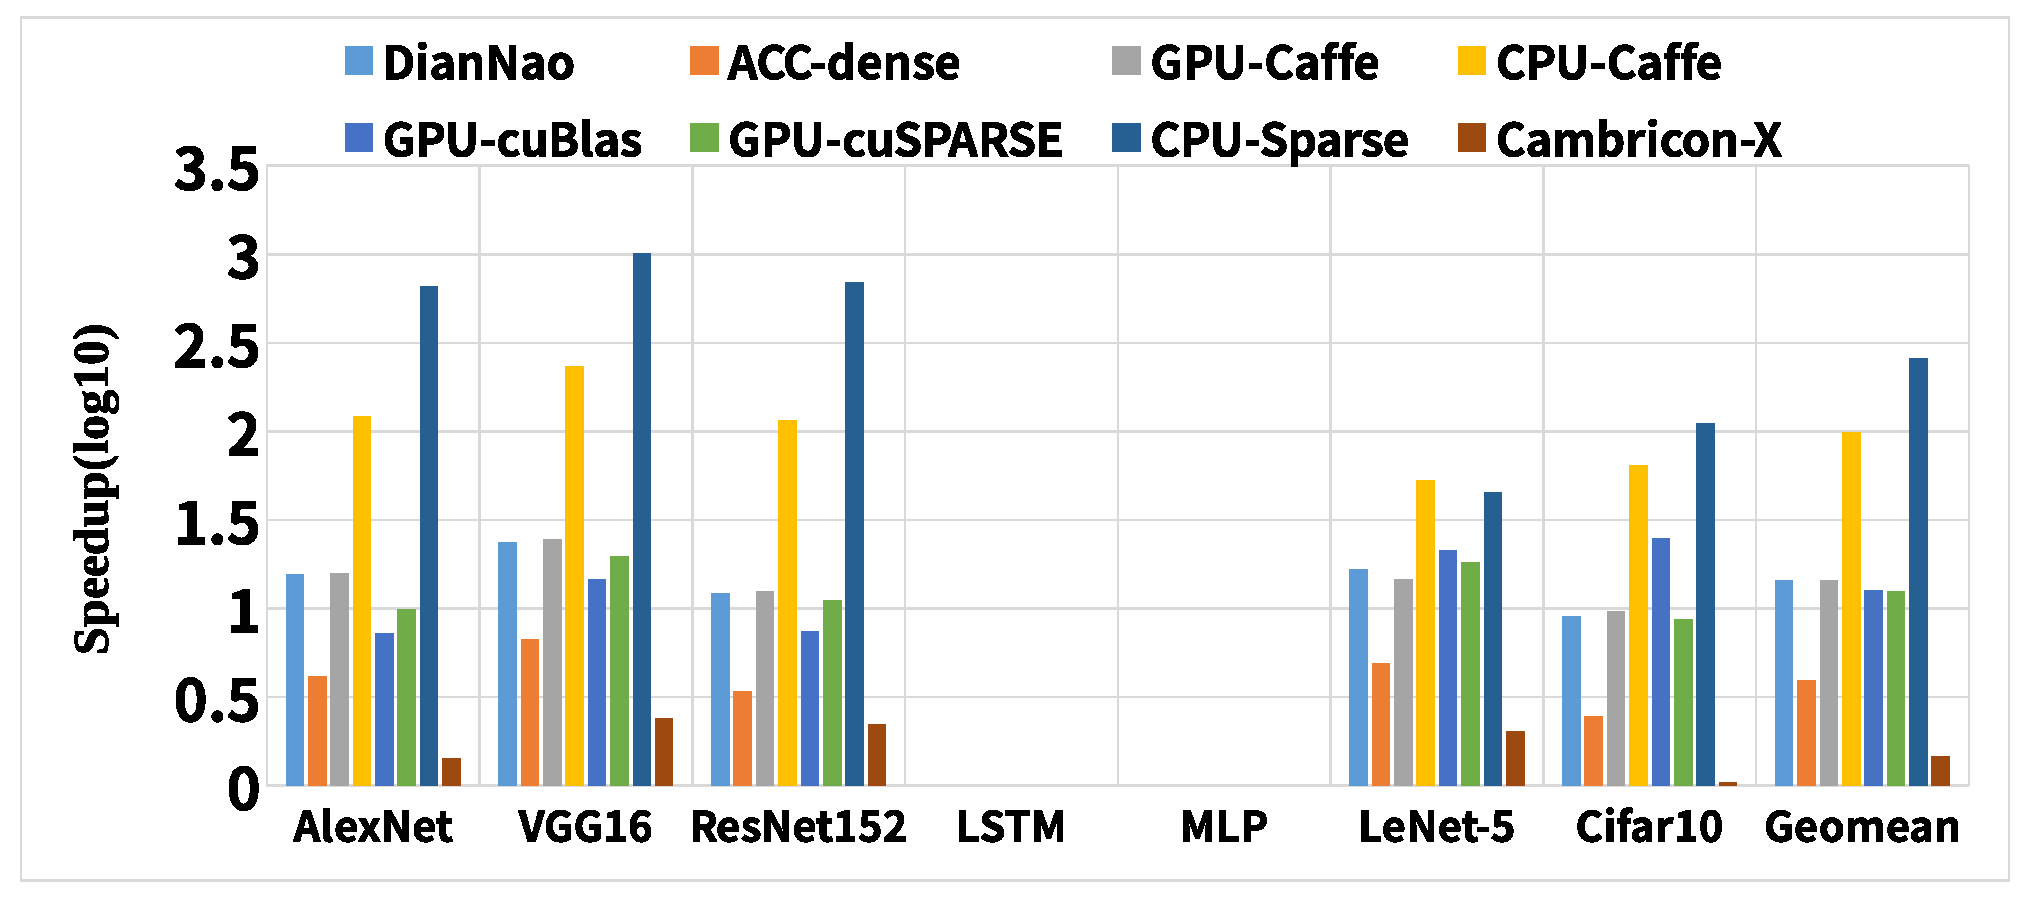
\includegraphics[width=0.8\columnwidth]{conv_performance.eps}
\caption{Cambricon-S与CPU,GPU,DianNao,Cambricon-X在卷积层上的性能对比}
\label{fig:conv_performance}
\end{figure}

\begin{figure}[h]
\centering
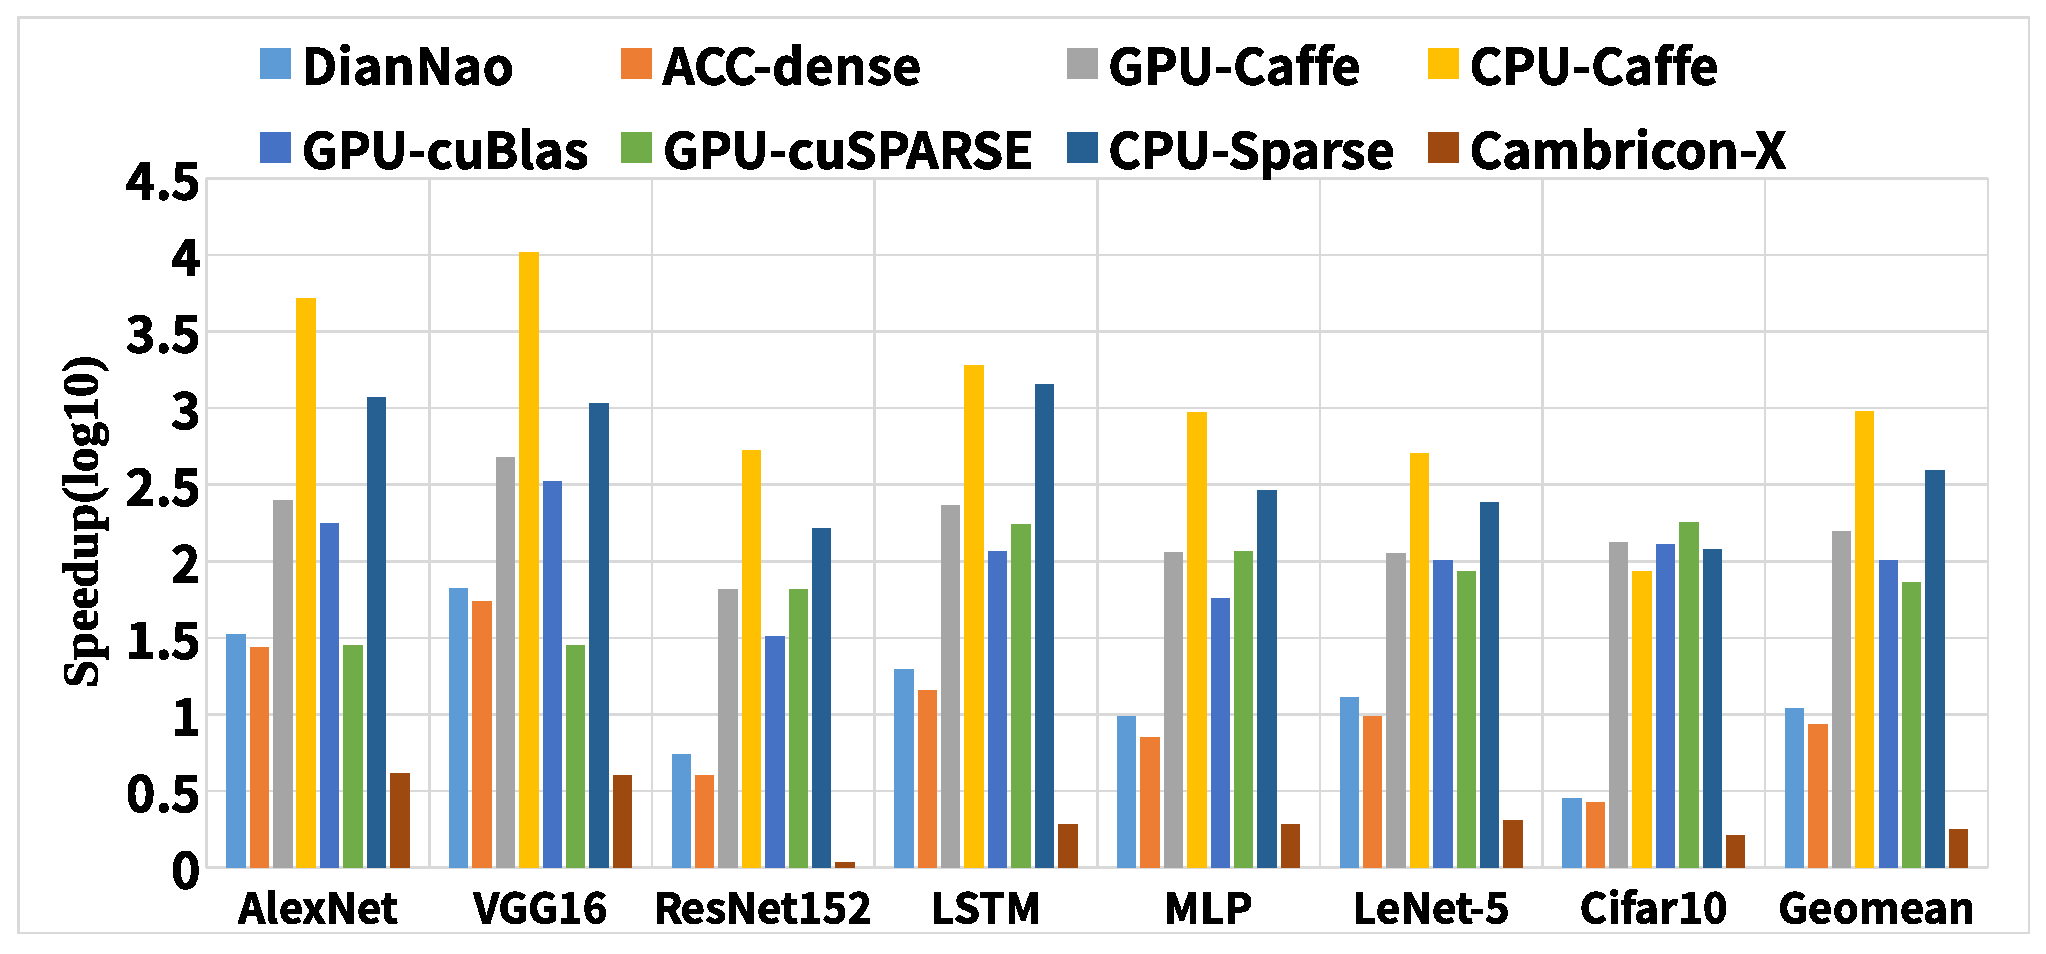
\includegraphics[width=0.8\columnwidth]{fc_performance.eps}
\caption{Cambricon-S与CPU,GPU,DianNao,Cambricon-X在全连接层上的性能对比}
\label{fig:fc_performance}
\end{figure}


在卷积层上的性能主要来源于SSM模块能够进一步挖掘神经元稀疏,因为卷积层是计算密集型的层,动态神经元稀疏可以大量减少神经网络中的计算量,例如在AlexNet网络的\emph{conv3}层,稠密情况下需要$52M$的MAC操作(Multiply–accumulate operation),而如果利用$45\%$的动态神经元稀疏,仅仅需要$29M$的MAC操作。

在全连接层的性能提升主要来源于权值存储量的减少(局部量化)和索引存储量的减少(索引共享)。WDM能够支持用户自定义比特长度的量化,从而减少突触的存储容量,获得1.77倍的加速比;粗粒度剪枝使得非零位置的索引信息能够被相邻多个输出神经元共享,因此能够额外获得1.21倍的加速比。


\subsection{能耗}
\begin{figure}[h]
\centering
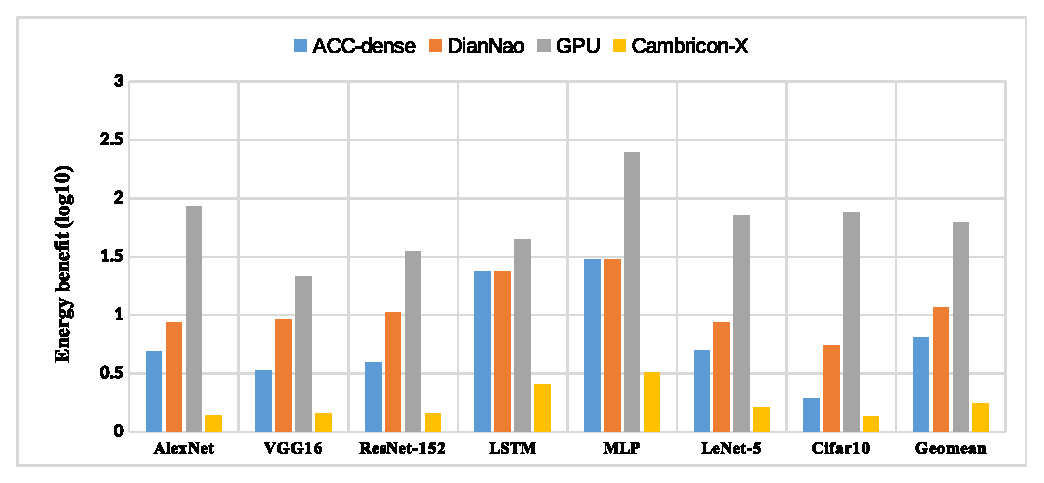
\includegraphics[width=0.8\columnwidth]{energy.eps}
\caption{新型加速器与GPU,DianNao,Cambricon-X在能耗的对比}
\label{fig:energy}
\end{figure}

\zadd{在七个benchmark上,我们比较了Cambricon-S,GPU,DianNao和Cambricon-X的能耗,其中我们包括了片外访存的能耗。如图~\ref{fig:energy}所示,对比于GPU,DianNao和Cambricon-X,Cambricon-S能够分别节约63.49倍,11.72倍和1.75倍的能耗。此外,我们观察到局部量化能够节约1.24倍的能耗,动态压缩神经元能够节约1.28倍的能耗。如果不考虑片外访存的能耗,Cambricon-S分别比GPU,DianNao和Cambricon-X节约1169.51倍,12.30倍和1.75倍能耗。以上实验数据证明我们的加速器能够使用很低的能耗完成神经网络的运算。
}


\begin{figure}[h]
\centering
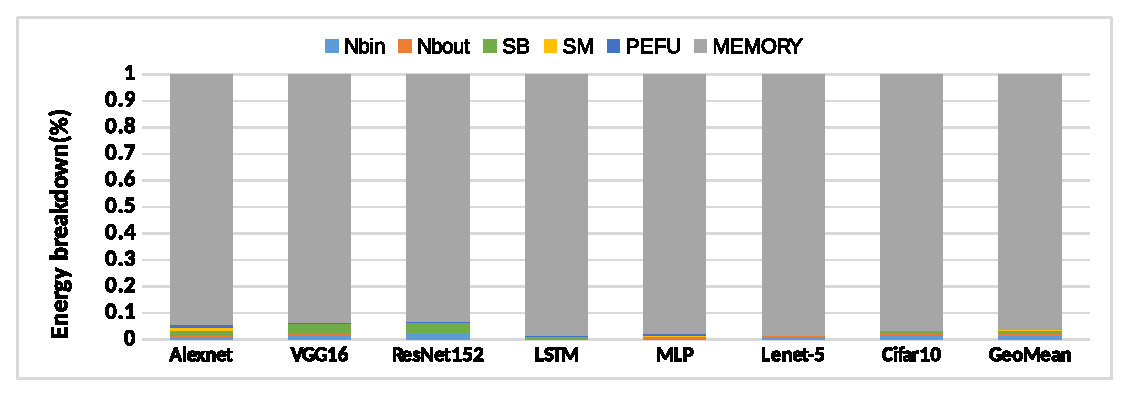
\includegraphics[width=0.8\columnwidth]{energy_breakdown.eps}
\caption{加速器在benchmark上的能耗分布(包括片外访存能耗)}
\label{fig:energy_breakdown}
\end{figure}

我们分析了加速器在七个benchmark上的能耗分布。如图~\ref{fig:energy_breakdown}所示,我们可以观察到片外访存消耗了超过$90\%$的总能量。在LSTM和MLP网络中,这个比例高达$98\%$,远高于其他神经网络,因此这两个网络是访存密集型的网络。实验结果显示,通过稀疏和量化可以显著减少片外访存的能耗。对比于稠密网络,稀疏网络能够减少$72.6\%$的片外访存能耗。

\begin{figure}[h]
\centering
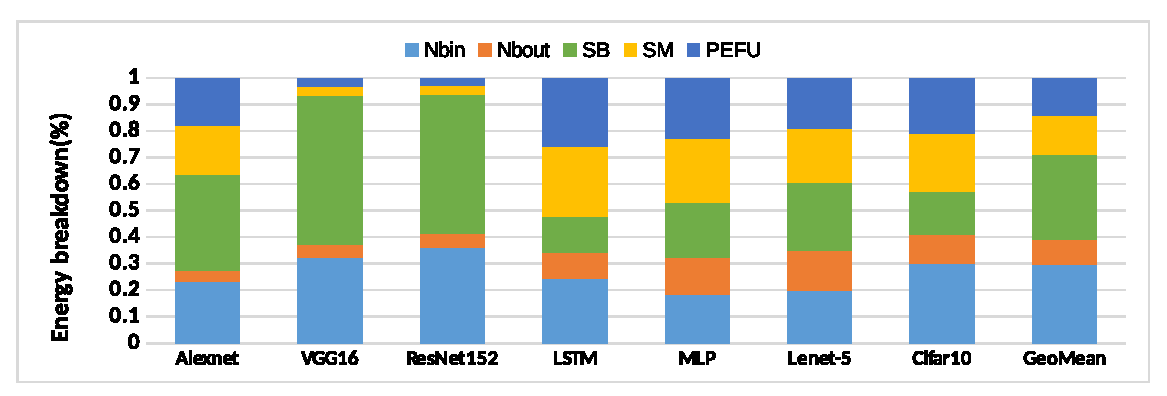
\includegraphics[width=0.8\columnwidth]{energy_breakdown2.eps}
\caption{加速器在benchmark上的能耗分布(不包括片外访存能耗)}
\label{fig:energy_breakdown2}
\end{figure}

我们进一步分析了在不包括片外访存能耗情况下加速器的能耗分布。如图~\ref{fig:energy_breakdown2}所示,片上缓存访问能耗(包括NBin,NBout和SB)平均消耗约$70\%$的总能量,这表明片上缓存访问能耗依然主导片上的能耗。对于LSTM和MLP这两个网络上,片上缓存能耗少于$60\%$,因为在这两个网络中权值不进行重用。对于深层的卷积网络,比如VGG16和ResNet152,片上内存访问能源的比例超过$90\%$,因为在这两个网络中需要复杂的loop tiling和数据重用策略将大规模运算映射到加速器熵。值得注意的是,与Cambricon-X相比,局部量化能够减少2.76倍的权值存储量,从而使得SB节约2.48倍的能耗。

\section{讨论}

\subsection{熵编码和熵解码模块}

目前Cambricon-S中并没有加入熵解码模块(entropy decoding module)来支持权值熵编码,主要是考虑到熵解码模块需要耗费非常大的面积和能耗,但是仅仅能够获得非常有限的性能提升。一个熵解码模块(entropy decoding module)的面积为$6.781*10^{-3}mm^2$,它能够在一个cycle解码出一个码字。由于熵编码是一种变长编码,因此对应的解码模块必须串行进行解码。即使我们可以将数据划分为许多并行的数据流,然后为每个数据流提供一个熵解码模块,这种方法将会引入巨大的面积和能耗开销。

考虑到每一个SB需要在一个cycle提供$T_m\times 4$个数据,为了避免性能损失,我们必须为一个SB提供$T_m\times 4$个熵解码模块,因此我们的加速器总共需要集成$T_n\times T_m\times 4$个熵解码模块。在$T_m = T_n = 16$的配置下,我们总共需要1024个熵解码模块,这将引入额外$6.94mm^2$的面积和$971.37mW$的功耗,因此加速器的总面积和功耗分别是$13.67mm^2$和$1769.92mW$,分别是原始设计的2.03倍和2.22倍。然而,新增熵解码的加速器在卷积层上几乎没有性能提升,在全连接层也只有1.18倍的性能提升,对比与额外的面积和功耗开销,这种性能提升是非常有限的。因此,我们在加速器中不加入熵解码模块。

\subsection{稀疏度与性能}
\begin{figure}[h]
\centering
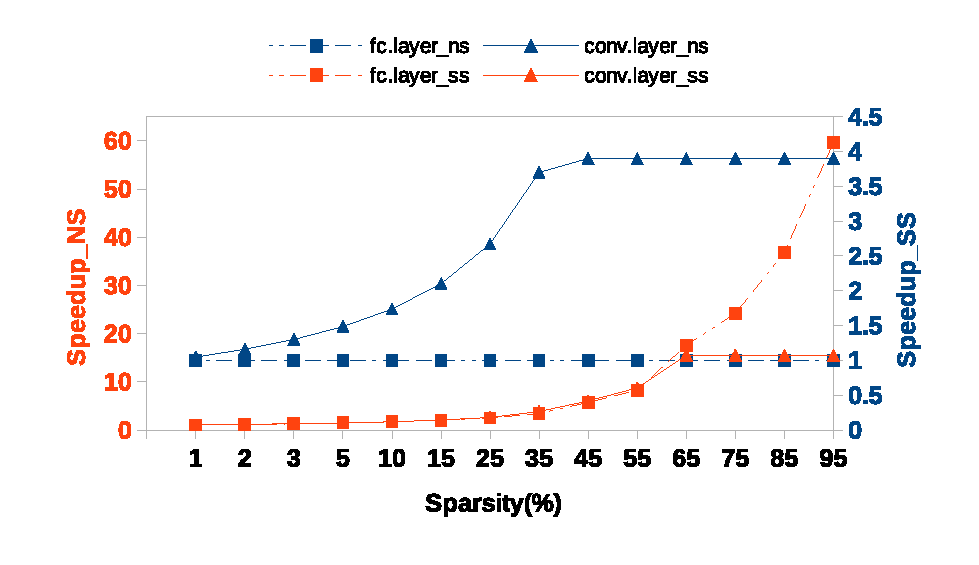
\includegraphics[width=0.8\columnwidth]{sensitivity.eps}
\caption{神经网络稀疏度对加速器性能的影响}
\label{fig:sensitivity}
\end{figure}

我们研究了Cambricon-S对神经网络稀疏度的敏感性,即稀疏度对神经网络性能的影响。如图~\ref{fig:sensitivity}所示,我们分别探究了神经元稀疏度和粗粒度权值稀疏度对加速器性能的影响,更进一步的,我们从卷积层和全连接层两个角度进行探究。从图中的数据我们观察到了几个有趣的实验结果:

1)考虑粗粒度权值稀疏,加速器能够在卷积层获得接近理想值的加速比(15.5倍 vs. 16倍)。为了兼容大多数网络的权值稀疏度(如表~\ref{tab:sparsities}所示),我们将NSM设计成为256选16的结构,即NSM最多从256个输入神经元中筛选出16个需要进行计算的神经元,从而最多实现16倍的加速器。我们的加速器能够接近理想加速器的主要原因是我们使用pingpong的模式管理片上缓存,使得加速器的片外访存延迟能够被运算时间覆盖。值得注意的是,由于我们的加速器能够充分利用粗粒度稀疏实现负载均衡,因此在相同稀疏度情况下,Cambricon-S能够获得比Cambricon-X更优的加速比。

2)考虑粗粒度权值稀疏,在全连接层中,Cambricon-S能够很容易地在低稀疏度情况下(低于$5\%$)获得加速比,并且随着稀疏度的提高,加速比也会不断提高,在稀疏度为$99\%$时能够获得59.59倍的加速比。主要原因是全连接层是一个访存密集的层,稀疏权值能够大大减少片外访存数据量,从而减少片外访存时间,减少总执行时间。

3)考虑神经元稀疏,Cambricon-S在卷积层最高能够获得3.9倍的加速比,接近理想的4倍加速比。由于在大多数情况下,神经元的稠密度高于$25\%$(稀疏度低于$75\%$),我们将SSM设计成为64选16的结构,因此最多获得4倍的加速比。这个设计能够满足绝大多数神经网络的需求。

4)神经元稀疏并不能在全连接层带来性能的提升,因此在全连接层片外权值访存时间主导了总执行时间(超过$99\%$),而神经元稀疏并不能有效地减少内存访问。

上述的实验结果进一步验证了我们的加速器能够高效地利用神经网络中神经元稀疏和权值稀疏。

\subsection{减少的不规则度}
减少稀疏神经网络的不规则度能够对加速器的设计,性能产生深远的影响。第一,减少不规则度能够简化加速器的设计。我们可以使用一个共享的NSM取代$T_n$个分布式的NSM,从而节省$10.35mm^2$的面积和$1821.9mW$的功耗;同时我们可以用一个共享的SIB来代替16个独立的SIB,从而节省$15KB$的SRAM大小。第二,减少不规则度能够大大减少权值索引的规模(26.83倍),减少片外访问权值,从而获得1.06倍的加速比,节约1.11倍的能耗。

\subsection{类似粗粒度稀疏的方法}
最近有不少类似于粗粒度稀疏的研究,例如SIMD-aware weight pruning~\cite{yu2017scalpel},synapse vector elimination~\cite{hill2017deftnn},channel reduction和filter reduction~\cite{wen2016learning,lebedev2016fast}。尽管这些技术可以减少稀疏神经网络的不规则度,从而简化加速器设计,但是通常会导致显著的精度损失~\cite{li2016pruning}。

\citet{mao2017exploring}探究了一系列结构化稀疏的方法,包括细粒度稀疏(fine-grained sparsity),向量层次稀疏(vector-level sparsity),卷积核层次稀疏(kernel-level sparsity)和过滤器层次稀疏(filter-level sparsity),同时评估这些稀疏方法对神经网络不规则度和精度的影响。 值得注意的是,我们提出的粗粒度剪枝方式并不会限制剪枝块的规模,因此是一种普遍性的剪枝方法。通过指定参数,粗粒度剪枝能够达到上述各种形式稀疏的效果。

\subsection{其他稀疏神经网络加速器}
EIE~\cite{han2016eie}能够加速稀疏神经网络的全连接层,它采用CSC的压缩方式压缩权值。为了能够完全消除片外访存,它使用非常大的片上缓存存储所有的突触。为了使AlexNet网络的全连接层权值能够完全存储在片上缓存,EIE的总面积需要达到$40.8mm^2$,是我们加速器的面积的5.07倍。同时,EIE只支持固定比特的量化,而新型加速器中的WDM能够支持自定义比特的量化,从而权衡神经网络的压缩效果和精度。为了公平地与EIE比较性能,我们假设加速器的片上缓存足够大,能够存储全连接层的所有权值,因此我们将加速器的性能聚焦在计算时间。如表~\ref{tab:EIE}所示,相比于EIE,新型加速器能够平均获得1.65倍的加速比。

\begin{table}[h]
\centering
\caption{\footnotesize Cambricon-S与EIE的性能比较 \emph{(microsecond)}.}
\label{tab:EIE}
\begin{tabular}{@{}lll@{~~}lll@{~~}lll@{~~}lll@{~~}lll@{~~}lll@{~~}lll@{~~}lllllll}
\toprule
layer & \multicolumn{3}{c}{AlexNet} & \multicolumn{3}{c}{VGG16} & Geomean\\
& fc6 & fc7 & fc8 & fc6 & fc7 & fc8     \\
\midrule
EIE & 30.30 & 12.20 & 9.90  & 34.40 & 8.70  & 7.50  & --\\
ACC & 18.43 & 8.19  & 5.13  & 25.23 & 4.12  & 5.09  & --\\
Speedup & $1.64\times$ & $1.49\times$ & $1.93\times$ & $1.36\times$ & $2.11\times$ & $1.49\times$ & $1.65\times$ \\
\bottomrule
\end{tabular}
\end{table}

我们的加速器与Cambricon-X~\cite{zhang2016cambricon}都是用了索引的方式利用神经网络的稀疏性质,但是Cambricon-S索引方式与Cambricon-X有三个方面不同。首先,Cambricon-S包含一个共享的索引模块(NSM),它能够充分挖掘权值的粗粒度稀疏特性。由于粗粒度稀疏,加速器的各个PE共享相同的索引,因此NSM筛选出的神经元能够被PE共享,从而减少索引模块开销以及NSM与PE之间的带宽需求。第二,Cambricon-S的PE中集成了一个本地的权值索引模块(SSM),从而充分利用神经元稀疏。虽然粗粒度稀疏能够减少稀疏神经网络的不规则性,但是稀疏的神经元依然存在不规则性,例如ReLU激励能够使得许多神经元的激励为“0”,SSM模块能够最小化这种不规则性的影响。因此新型索引模块能够充分利用神经元稀疏和权值稀疏,而Cambricon-X只能利用权值稀疏。第三,Cambricon-S中集成了Encoder模块,动态压缩稀疏的神经元,从而减少片外神经元访问。实验显示,Encoder模块能够进一步节约1.28倍的能耗;更具体地说,它能够在卷积层和全连接层分别节约1.68倍和1.02倍的能耗。第四,Cambricon-S的每一个PE中集成了WDM模块用于解码量化后的权值,从而充分利用局部量化,进一步减少片外权值访问量。

\zadd{SCNN~\cite{angshuman2017scnn}能够挖掘权值稀疏和神经元稀疏,对比于稠密神经网络,它能够获得2.7倍的加速比,同时节约2.3倍的能耗。而我们加速器能够获得4.32倍的加速比,节约6.53倍的能耗,这充分显示了我们加速器高性能和低能耗的特点。Cambricon-S在处理稀疏神经网络时能够获得4.32倍的加速比,这部分的性能提升主要来自于三个方面。首先,NSM可以充分利用突触稀疏(平均权值稀疏度为$87.99\%$)从而减少计算,最终实现2.06倍的加速比。第二,SSM能够充分利用神经元稀疏(平均神经元稀疏度为$55.41\%$),从而减少神经网络所需的计算量,最终获得1.44倍的加速比。第三,粗粒度稀疏($78.99\%$)和局部量化(减少2.76倍突触数据)可以大大减少片外权值访问量,从而获得1.46倍的加速比。
}

\section{本章小结}
\zadd{在本章,我们评估了Cambricon-S的性能和能耗。}
    
\zadd{我们首先介绍了实验工具链,实验平台,baseline和benchmark。在$65nm$工艺下,Cambricon-S的面积和功耗仅仅为$6.82mm^2$和$821.19mW$。
我们在七个benchmark上分别比较了CPU,GPU,DianNao,Cambricon-X和Cambricon-S的性能和能耗,我们发现Cambricon-S具有高性能和低能耗的特点。与最先进的稀疏的神经网络加速器Cambricon-X相比,Cambricon-S能够获得1.71倍的加速比,同时节约1.75倍的能耗。
}

\zadd{
最后,我们详细讨论了Cambricon-S的一些特性,我们发现在加速器中集成熵解码模块会耗费非常大的面积和能耗,但是不能获得非常理想的性能提升,因此我们不在加速器中集成熵解码模块。同时,我们发现加速器能够高效地利用神经网络中神经元稀疏特性和权值稀疏特性,且对稀疏特性的利用率高于Cambrcion-X,EIE和SCNN。}



\chapter{总结和展望}

\section{本文工作总结}
人工神经网络近年来在学术界和工业界获得迅猛发展,目前神经网络已经成为众多领域,包括图像识别、物体检测、语音处理和自然语言处理等获得非常理想的效果。神经网络的功能不断增强的过程中,规模不断扩大,层数不断加深,因此神经网络需要庞大的存储资源,计算资源和能耗完成运算。因此研究者采用剪枝的方法将神经网络稀疏化,从而减少神经网络参数和计算量。但是稀疏神经网络的不规则性会使得CPU,GPU和大部分神经网络加速器无法利用稀疏性获得性能提升,尽管有一部分加速器能够支持稀疏特性,但是开销较大,而且效果并不理想。因此本文提出了一种软硬件结合的方法处理稀疏神经网络的不规则性,从算法和架构设计的角度提出多种优化策略,显著提升处理稀疏神经网络的效果。本文的主要创新点体现在一下几个方面:

\textbf{1.软硬件结合的方法处理稀疏神经网路的不规则性。}本文首次提出采用软硬件结合的方法处理稀疏神经网络不规则性。在软件方面我们提出了一种新的神经网络剪枝方法,即粗粒度剪枝,对神经网络进行粗粒度稀疏,从而减少稀疏神经网络的不规则形;在硬件方面,我们提出了Cambricon-S来高效处理粗粒度稀疏和动态神经元稀疏,从而更加有效地利用稀疏性,获得性能的提升。

\textbf{2.基于局部收敛的神经网络压缩算法。}本文通过大量的实验,观察到了局部收敛的现象,即神经网络的权值不是一种随机分布的情况,而是在训练过程中大的权值会聚集成簇。本文根据观察到的局部收敛现象,提出了一种新的神经网络压缩算法。压缩算法包括三个步骤,分别是粗粒度剪枝,局部量化和熵编码。粗粒度剪枝将神经网络的权值分为多个权值块,当一个权值块符合某个条件时将从网络拓扑中被完全剪除,粗粒度剪枝能够显著减少稀疏的神经网络的不规则度。局部量化将权值分为多个子区域,然后在每一个子区域内分别进行量化,从而降低表示权值的比特数,进一步压缩神经网络。之后,我们采用熵编码对神经网络进行无损压缩。新的神经网络压缩算法不仅能够降低稀疏神经网络的稀疏度,获得非常理想的压缩比,还能降低稀疏神经网络的不规则度。粗粒度剪枝可以将稀疏神经网络不规则性平均减少20.13倍。受益于粗粒度稀疏和局部量化,我们新的压缩方法可以将AlexNet和VGG分别压缩79倍和98倍,远远高于目前最先进的两个神经网络压缩算法Deep Compression (35倍/49倍) 和 CNNPack (39倍/46倍)。

\textbf{3.高效处理压缩神经网络的神经网络加速器。}本文设计并提出了首个能够支持粗粒度稀疏神经网络的加速器微结构Cambricon-S。该微结构的主要的特征是一个共享的神经元选择模块NSM,用来挖掘粗粒度权值稀疏的特性,即神经元共享和索引信息共享。同时微结构还包括SSM,Encoder和WDM,分别用来处理动态神经元稀疏,动态压缩神经元和解码经过局部量化的权值。新型加速器不仅能够处理普通的稠密神经网络,还能够通过打开/关闭稀疏处理模块支持多种稀疏/量化情况,包括神经元稀疏,粗粒度权值稀疏,神经元/权值同时稀疏情况,局部量化等。新型加速器能够非常高效的利用稀疏和量化,获得非常理想的性能和非常低的能耗。
同时,为了减少用户的编程负担,我们为加速器设计了专用的基于库的编程模型。编程模型中集成了加速器专用的编译器,能够将C++高级语言编译成为加速器可执行指令;值得注意的,编译器能够静态分析指令之间的依赖关系,提取出没有依赖关系的指令,使它们能够在加速器中同时进行发射。
在65nm工艺下,加速器的总面积和总功耗分别是 $6.82mm^2$ 和 $821.19mW$,工作频率为$1GHz$,吞吐量为$512GOP/s$,片上 SRAM共为$54KB$。实验结果显示,对比目前最先进的稀疏神经网络加速器Cambricon-X,新型加速器能够获得1.71倍的性能提升,同时降低1.75倍的能耗。

\section{未来研究展望}

本文提出了软硬件结合的方法处理稀疏神经网络的不规则性。在软件上,粗粒度稀疏减少了神经网络的不规则度,同时新的压缩算法能够深度压缩神经网络,取得非常理想的压缩比。在硬件上,新型加速器能够处理粗粒度稀疏神经网络,相比以前的稀疏神经网络加速器能够进一步提升性能,降低能耗。

未来神经网络处理器的发展主要会聚焦在两个方面,分别是嵌入式系统领域和云端处理领域。

\textbf{高性能,低功耗的神经网络芯片。}
针对嵌入式设备中的神经网络应用,未来的工作可以从两个方面入手。一方面,在算法方面,我们可以通过裁剪网络,量化,低精度计算等方法,在精度损失允许的范围内,减少神经网络的参数数量和计算量,从而使得神经网络的规模能够部署到嵌入式设备中。另一个方面,我们需要设计特定的神经网络处理器,使其能够支持多种神经网络优化算法,如稀疏,量化等,从而获得高性能的同时降低能耗。

\textbf{高吞吐量,低延迟的多核神经网络处理器。}
随着越来越多的神经网络算法部署到云端,云计算(cloud computing)必须能够保证神经网络运算的服务质量(Quality of Service,QoS)的同时,最小化资源消耗。针对神经网络应用的云服务,未来的工作可以从两个方面进行优化。一方面,在底层硬件方面,我们可以设计高吞吐量,低延迟的多核神经网络处理器,并将其部署到云端来代替传统的CPU和GPU,为神经网络应用提供服务。设计多核神经网络处理器会涉及到诸多设计选择(design choice)的问题,如单核处理器的框架的选择,片上网络(network on chip, NoC)的设计(包括核之间如何互联,核与存储器之间如何路由等),存储设计问题(如存储器层次划分,存储器容量,片上缓存选择Cache的形式还是Stratch-pad的形式等)。另一方面,在上层软件支撑方面,我们需要针对神经网络应用的特点和底层硬件的特点,设计针对云端神经网络应用的编程框架。编程框架中的一个核心问题就是调度问题,即如何将神经网络应用部署到底层硬件中,保证应用的QoS需求,同时最小化资源的消耗。




\bibliography{bib/ustc}

%\appendix

\backmatter
\begin{acknowledgements}
不知不觉博士生涯就要结束了,在这五年半的时间里,我在许多城市,包括合肥,苏州,北京,上海等进行学习,我遇到了很多帮助我的老师和同学,在这里,我向他们表达最真诚的谢意。

首先要感谢我的导师周学海教授,前两年半的博士生涯,是周老师一步一步带着我进行体系结构的学习,带我进入了计算机体系结构的大门,让我领略了体系结构的魅力。周老师让不管在生活上还是在研究上都充满了大智慧,特别是在研究上,能够在high-level的角度一针见血地点出问题的本质。周老师在2016年年初将我推荐到计算所陈老师的国重实验室(智能处理器研究中心)进行深入学习,使我能够接触最前沿的科学研究,非常感谢周老师当时的决定。

其次,我要感谢计算所的陈云霁研究员。陈老师学识渊博,平易近人,能够处处为学生着想,为学生创造一个非常良好的学习和工程的环境。我还记得当时和陈老师一起通宵写课题,一起爬山,打桌游,吃火锅的时光。在北京计算所的一年时间里,我学到了许多知识,包括工程方面,如前端设计,前端验证,驱动编写等;还包括科研方面,包括神经网络算法知识,性能分析,加速器架构设计等。

同时我要感谢杜子东老师。在2017年,我加入了杜老师的前瞻组,并在接下来的一年半时间里在上海寒武纪分部专心进行科研。杜老师领我进入了科研的大门,帮我培养学术上的思维习惯,教我如何选择idea,组织文章结构,呈现硬件架构,呈现实验结果,进行性能分析,能耗分析等,从而完成一篇高质量的论文。杜老师为人师表,在科研上孜孜不倦,认真负责,在杜老师的帮助下,最终让我达到了毕业的要求。

另外,我要感谢嵌入式系统实验室的李曦老师,陈香兰老师,王超老师对我的指导。同时还要感谢寒武纪陈天石老师,刘少礼老师,王在老师,喻歆老师,郭琦老师,刘道福老师,罗韬老师,支天老师和软件所的李玲老师等对我生活上,工程上和学术上的帮助。

同时,感谢嵌入式系统实验室的师兄师弟们,特别感谢周金红师兄,余奇,马翔,万波,李俊,陈航,赵勇对我的帮助。感谢在寒武纪和我一起工作的同学们:兰慧盈,周聖元,刘雨辰,韩栋,李震,张士锦等对我的照顾,跟大家一起学习,做工程,做研究真的学到了很多。

最后,感谢我的父母和亲人,成长就是最好的报答。

\end{acknowledgements}

\begin{publications}

\section*{已发表论文}

\begin{enumerate}
\item A A A A A A A A A
\item A A A A A A A A A
\item A A A A A A A A A
\end{enumerate}

\section*{待发表论文}

\begin{enumerate}
\item A A A A A A A A A
\item A A A A A A A A A
\item A A A A A A A A A
\end{enumerate}

\section*{研究报告}
\begin{enumerate}
\item A A A A A A A A A
\item A A A A A A A A A
\item A A A A A A A A A
\end{enumerate}

\end{publications}


\end{document}
